\documentclass[12pt]{article}
\usepackage[utf8]{inputenc}
\usepackage{amsmath}
\usepackage{csquotes}
\usepackage[ruled,vlined]{algorithm2e}
\usepackage{amssymb}
\usepackage{parskip}
\usepackage{graphicx}
\usepackage{epstopdf}
\usepackage{subcaption}
\usepackage{listings}
\usepackage{url}
\usepackage{cite}
\usepackage{caption}
\usepackage{mathtools}
\usepackage{physics}
\usepackage{bm}
\usepackage{float}
\usepackage{fp}
\usepackage{amssymb}
\usepackage{pdfpages}
\DeclareMathOperator{\E}{\mathbb{E}}
\DeclareMathOperator{\Var}{\mathbb{V}}
\DeclareMathOperator{\Cov}{\mathbb{C}\text{ov}}
\usepackage{graphicx}
\usepackage{subcaption}
\usepackage{mwe}
\usepackage{subfigure}
\usepackage{rotating}
\usepackage{graphicx,color,psfrag}
\usepackage{longtable}
\usepackage{multirow}
\usepackage{amsmath}
\usepackage{breqn}
\usepackage{overpic}
\usepackage{framed}
\usepackage{color}
\usepackage{fontspec}
\usepackage{xcolor}
\usepackage{diagbox}
\usepackage{algorithm}  
\usepackage{algorithmic}
\makeatletter
\usepackage{titlesec}

\lst@CCPutMacro
    \lst@ProcessOther{"2D}{-{}}
    \@empty\z@\@empty
\makeatother
\lstset{
    columns=fixed,       
    numbers=left,                                        % 
    frame=none,                                          % 
    backgroundcolor=\color[RGB]{245,245,244},            % 
    keywordstyle=\color[RGB]{40,40,255},                 % 
    numberstyle=\scriptsize\color{darkgray},           % 
    commentstyle=\it\color[RGB]{0,96,96},                % 
    stringstyle=\rmfamily\slshape\color[RGB]{128,0,0},   % 
    showstringspaces=false,                              % 
    language=matlab,                                        % 
}



\setmainfont{Times New Roman}
\numberwithin{equation}{section}
\numberwithin{figure}{section}
% Default fixed font does not support bold face
\DeclareFixedFont{\ttb}{T1}{txtt}{bx}{n}{12} % for bold
\DeclareFixedFont{\ttm}{T1}{txtt}{m}{n}{12}  % for normal

% Custom colors
\usepackage{color}
\definecolor{deepblue}{rgb}{0,0,0.5}
\definecolor{deepred}{rgb}{0.6,0,0}
\definecolor{deepgreen}{rgb}{0,0.5,0}


\newfontfamily\sectionef{Times New Roman}
\titleformat*{\section}{\Large\sectionef\bfseries}
\titleformat*{\subsection}{\large\sectionef\bfseries}
\titleformat*{\subsubsection}{\normalsize\sectionef\bfseries}




\usepackage{times}



\usepackage{geometry}
\usepackage[normalem]{ulem}
\useunder{\uline}{\ul}{}
\linespread{1.5}

%Includes "References" in the table of contents
\usepackage[nottoc]{tocbibind}




\geometry{a4paper,left=2cm,right=2cm,top=2cm,bottom=2.5cm}
% head
\topskip=0.5cm
\usepackage{fancyhdr}
\pagestyle{fancy}
\lhead{
\includegraphics[scale=0.5]{figures/dtu_logo.pdf}} 

\chead{}
\rhead{\setmainfont{Courier New Bold} \bfseries 02612 Constrained Optimization}
%%%%%%%%%%%%%%%%%%%%%%%%%%%%%%%%%%%%%%%%%%%%%%%%%%%%%
\usepackage[CJKbookmarks=true]{hyperref}



\begin{document}
%----------------------------------------------------------------------------------------
%	TITLE PAGE
%----------------------------------------------------------------------------------------


\begin{titlepage}

\newcommand{\HRule}{\rule{\linewidth}{0.5mm}} % Defines a new command for the horizontal lines, change thickness here

\center % Center everything on the page
 
%----------------------------------------------------------------------------------------
%	HEADING SECTIONS
%----------------------------------------------------------------------------------------

 % Name of your university/college
%\textsc{\Large Clinical Engineering }\\[0.5cm] % Major heading such as course name
%\textsc{\large Minor Heading}\\[0.5cm] % Minor heading such as course title



%----------------------------------------------------------------------------------------
%	TITLE SECTION
%----------------------------------------------------------------------------------------

\HRule \\[0.8cm]
{\Large \bfseries02612 Constrained Optimization}\\[0.4cm]
{\huge \bfseries \ Assignment Report}
% Title of your document
%\textsc{\Huge \bfseries LEGO}\\[0.4cm]
% Title of your document
\HRule \\[0.5cm]
\vspace{1.5cm}


 %----------------------------------------------------------------------------------------
%	LOGO SECTION
%----------------------------------------------------------------------------------------


\includegraphics[width=0.2\textwidth]{figures/DTUlogo.png}\\[1.8cm] % Include a department/university logo - this will require the graphic package
 
%----------------------------------------------------------------------------------------
%	AUTHOR SECTION
%----------------------------------------------------------------------------------------



%%%They suggest to sort authors according to student number.
\begin{table}[H]
\centering
\begin{tabular}{cccc}
\textbf{Authors} & \textbf{Student Number}\\
Haotian Gao & s192232\\

\\
\end{tabular}
\end{table}
%----------------------------------------------------------------------------------------
%	DATE SECTION
%----------------------------------------------------------------------------------------

%{\centering May 8^{\text{th}}, 2019} % Date, change the \today to a set date if you want to be precise

%\end{localsize}
%----------------------------------------------------------------------------------------
\vfill % Fill the rest of the page with white space
May, \textbf{2020}\\[0.2cm] 
Technical University of Denmark\\[0.2cm]
\end{titlepage}
\pagenumbering{roman}
\tableofcontents
\clearpage
\pagenumbering{arabic}

\section{ \bfseries Equality Constrained Convex QP}

\begin{align*}
&\min_{x} \quad \phi=\frac{1}{2} x^{\prime} H x+g^{\prime} x \tag{1}\label{con:op1}\\
& s.t. \quad A^{\prime} x=b\\
&\text{with}\quad H \succ 0
\end{align*}



%%%%%%%%%%%%%%%%%%%%%%%%%%%%%%%%%%%%%%%%%%
%%%%%%%%%%%%%%%%%%%%%%%%%%%%%%%%%%%%%%%%%%%%%%%%%%%%%%%%%%%%%%%%%%%%%%%%%%%%%%%%%%%%%
%%%%%%%%%%%%%%%%%%%%%%%%%%%%%%%%%%%%%%%%%%%
%%%%%%%%%%%%%%%%%%%%%%%%%%%%%%%%%%%%%%%%%%
%%%%%%%%%%%%%%%%%%%%%%%%%%%%%%%%%%%%%%%%%%%
\subsection{\bfseries Lagrangian function}
\definecolor{shadecolor}{rgb}{0.92,0.92,0.92}
\begin{shaded}
{ Question: What is the Lagrangian function for this problem?}
\end{shaded}
\begin{align*}
L(x, \lambda)&=f(x)-\sum_{i \in \mathcal{E}} \lambda_{i} c_{i}(x)\\
&=\frac{1}{2} x^{\prime} H x+g^{\prime} x-\lambda^{\prime}(A^{\prime}x-b)
\end{align*}




%%%%%%%%%%%%%%%%%%%%%%%%%%%%%%%%%%%%%%%%%%
%%%%%%%%%%%%%%%%%%%%%%%%%%%%%%%%%%%%%%%%%%%
%%%%%%%%%%%%%%%%%%%%%%%%%%%%%%%%%%%%%%%%%%
%%%%%%%%%%%%%%%%%%%%%%%%%%%%%%%%%%%%%%%%%%%
%%%%%%%%%%%%%%%%%%%%%%%%%%%%%%%%%%%%%%%%%%
%%%%%%%%%%%%%%%%%%%%%%%%%%%%%%%%%%%%%%%%%%%
\subsection{\bfseries Optimality conditions}
\begin{shaded}
{Question: What is the first order necessary optimality conditions for this problem? Are they
also sufficient and why?}
\end{shaded}
\bm{$Theorem\ (Necessary\ 1st\  Order\  Conditions)$}\\
Let x be a local minimizer of (\ref{con:op1}). Then
\begin{flalign}
&\ 1.\ \nabla_{x} L\left(x,\lambda\right)=Hx+g-A\lambda=0&\\
&\ 2.\ c_{i}\left(x\right)=A^{\prime}x-b=0 \quad i \in \mathcal{E}&
\end{flalign}
The constrained optimization problem (\ref{con:op1}) is convex because\\[0.3cm]
\ 1.\ $\phi$ is convex\ (H is positive definite).\\
\ 2.\ The equality constraints are linear.\\[0.3cm]
So the first order optimality conditions are sufficient for this problem. 




%%%%%%%%%%%%%%%%%%%%%%%%%%%%%%%%%%%%%%%%%%
%%%%%%%%%%%%%%%%%%%%%%%%%%%%%%%%%%%%%%%%%%%%%%%%%%%%%%%%%%%%%%%%%%%%%%%%%%%%%%%%%%%%%
%%%%%%%%%%%%%%%%%%%%%%%%%%%%%%%%%%%%%%%%%%%
%%%%%%%%%%%%%%%%%%%%%%%%%%%%%%%%%%%%%%%%%%
%%%%%%%%%%%%%%%%%%%%%%%%%%%%%%%%%%%%%%%%%%%
\newpage
\subsection{\bfseries Solvers implementation}
\begin{shaded}
{Question: Implement solvers for solution of the problem (1.1) that are based on an LU-factorization (dense), LU-factorization (sparse), LDL-factorization (dense), LDL-factorization (sparse), a range-space factorization, and a null-space factorization.
You must provide pseudo-code and source code for your implementation.}
\end{shaded}
Through the the first order optimality conditions listed, The convex equality constrained QP is solved by solution of the
KKT system\\
$$\overbrace{\begin{bmatrix}
H & -A\\
-A^{\prime} & 0
\end{bmatrix}}^{=KKT_{A}}
\overbrace{
\begin{bmatrix}
x\\
\lambda
\end{bmatrix}}^{=z}=
\overbrace{
-\begin{bmatrix}
g\\
b
\end{bmatrix}}^{=KKT_b}\eqno{(1.3)}$$\\[0.3cm]
Then the methods to factorize the KKT system are discussed. Please find the interface function "EqualityQPSolver" which can switch between the different solvers in the Appendix section \ref{6.1.1}.





%%%%%%%%%%%%%%%%%%%%%%%%%%%%%%%%%%%%%%%%%%
%%%%%%%%%%%%%%%%%%%%%%%%%%%%%%%%%%%%%%%%%%%
\subsubsection{\bfseries LU factorization (dense)}
Assuming that the $KKT_A$ is a square and nonsingular matrix. The LU factorization can be used with partial pivoting to decompose the matrix $KKT_A$ into an upper triangular matrix U, a lower triangular matrix L, and a permutation matrix P such that\\
$$PA=LU$$
Then backward and forward substitution can be performed with the triangular factors. But this method has the disadvantage that it ignores the symmetry. In the implementation, LU-factorization returns the row permutations p as a vector instead of a matrix P in order to save the memory. 

{\setmainfont{Courier New Bold} \scriptsize        
\begin{lstlisting}
function [x,lambda]=EqualityQPSolverLUdense(H,g,A,b)
%EqualityQPSolverLUdense  Equality constrained convex QP
%Syntax: [x,lambda]=EqualityQPSolverLUdense(H,g,A,b)

%dimension of A>>>>>number of x and equality constraints
[nx,nc]=size(A);
%setup KKT system(dense)
KKT_A=[H -A;-A' zeros(nc,nc)];
KKT_b=-[g;b];
% factorize and solve KKT system using the LU factorization
[L,U,p]=lu(KKT_A,'vector');
z=U\(L\KKT_b(p));
%Extract solution
x=z(1:nx);
lambda=z(nx+1:end);
end
\end{lstlisting}}

%%%%%%%%%%%%%%%%%%%%%%%%%%%%%%%%%%%%%%%%%%
%%%%%%%%%%%%%%%%%%%%%%%%%%%%%%%%%%%%%%%%%%%
\subsubsection{\bfseries LU factorization (sparse)}
Compared with the LU factorization(dense), The KKT matrix is represented as a sparse matrix.

{\setmainfont{Courier New Bold}      \scriptsize       
\begin{lstlisting}
function [x,lambda]=EqualityQPSolverLUsparse(H,g,A,b)
%EqualityQPSolverLUsparse Equality constrained convex QP

%Syntax: [x,lambda]=EqualityQPSolverLUsparse(H,g,A,b)

%dimension of A>>>>>>number of x and equality constraints
[nx,nc]=size(A);
%setup KKT system(dense)
KKT_A=[H -A;-A' zeros(nc,nc)];
KKT_b=-[g;b];
%sparse KKT system
KKT_A=sparse(KKT_A);
KKT_b=sparse(KKT_b);
% factorize and solve KKT system using the LU factorization
[L,U,p]=lu(KKT_A,'vector');% factorization
z=U\(L\KKT_b(p));% back substitution
%Extract solution
x=z(1:nx);
lambda=z(nx+1:end);
end
\end{lstlisting}}



%%%%%%%%%%%%%%%%%%%%%%%%%%%%%%%%%%%%%%%%%%
%%%%%%%%%%%%%%%%%%%%%%%%%%%%%%%%%%%%%%%%%%%
\subsubsection{\bfseries LDL factorization (dense)}
For a symmetric positive definite matrix $KKT_A$, the factorization has the form
$$P^{\prime}(KKT_A)P=LBL^{\prime}\eqno{(1.4)}$$
where P is the permutation matrix, L is the lower triangular matrix and B is a block diagonal
matrix. The symmetric permutation defined by the matrix P are introduced for numerical sability of the computation.

{\setmainfont{Courier New Bold}  \scriptsize           
\begin{lstlisting}
function [x,lambda]=EqualityQPSolverLDLdense(H,g,A,b)
%EqualityQPSolverLDLdense  Equality constrained convex QP

%Syntax: [x,lambda]=EqualityQPSolverLDLdense(H,g,A,b)

%dimension of A>>>>>>>number of x and equality constraints
[nx,nc]=size(A);
%setup KKT system(dense)
KKT_A=[H -A;-A' zeros(nc,nc)];
KKT_b=-[g;b];
% factorize and solve KKT system using the LDL factorization
z=zeros(nx+nc,1);
[L,D,p]=ldl(KKT_A,'vector');% factorization
z(p)=L'\(D\(L\KKT_b(p)));% back substitution
%Extract solution
x=z(1:nx);
lambda=z(nx+1:end);
end
\end{lstlisting}}



%%%%%%%%%%%%%%%%%%%%%%%%%%%%%%%%%%%%%%%%%%
%%%%%%%%%%%%%%%%%%%%%%%%%%%%%%%%%%%%%%%%%%%
\subsubsection{\bfseries LDL factorization (sparse)}
Compared with the LDL factorization(dense), The KKT matrix is represented as a sparse matrix

{\setmainfont{Courier New Bold}   \scriptsize          
\begin{lstlisting}
function [x,lambda]=EqualityQPSolverLDLsparse(H,g,A,b)
%EqualityQPSolverLDLsparse  Equality constrained convex QP

%Syntax: [x,lambda]=EqualityQPSolverLDLsparse(H,g,A,b)

%dimension of A------>number of x and equality constraints
[nx,nc]=size(A);
%setup KKT system(dense)
KKT_A=[H -A;-A' zeros(nc,nc)];
KKT_b=-[g;b];
%sparse KKT system
KKT_A=sparse(KKT_A);
KKT_b=sparse(KKT_b);
% factorize and solve KKT system using the LDL factorization
z=zeros(nx+nc,1);
[L,D,p]=ldl(KKT_A,'vector');% factorization
z(p)=L'\(D\(L\KKT_b(p)));% back substitution
%Extract solution
x=z(1:nx);
lambda=z(nx+1:end);
end
\end{lstlisting}}



%%%%%%%%%%%%%%%%%%%%%%%%%%%%%%%%%%%%%%%%%%
%%%%%%%%%%%%%%%%%%%%%%%%%%%%%%%%%%%%%%%%%%%
\subsubsection{\bfseries Range-Space factorization}
Assume that the KKT system\\
$$\begin{bmatrix}
H & -A\\
-A^{\prime} & 0
\end{bmatrix}
\begin{bmatrix}
x\\
\lambda
\end{bmatrix}=
-\begin{bmatrix}
g\\
b
\end{bmatrix} \quad A \in \mathbb{R}^{n \times m}$$\\[0.3cm]
The Range-Space method is useful when\\
1.$H$ is well-conditioned and easy to invert ($H$ is diagonal or block-diagonal).\\
2.$H^{\prime}$ is known explicitly.\\
3.The number of equality constraints (m) is small.\\[0.3cm]
From the KKT system
$$Hx-A\lambda=-g \quad \Leftrightarrow \quad x=H^{-1}A\lambda-H^{-1}g$$
Substitute it into second equation
\begin{align*}
b=A^{\prime}x&=\left(A^{\prime}H^{-1}A\right)\lambda-A^{\prime}H^{-1}g\\
\lambda&=\left(A^{\prime}H^{-1}A\right)^{-1}\left(b+A^{\prime}H^{-1}g\right)
\end{align*}\\[0.3cm]
{\setmainfont{Times New Roman}\bfseries Pseudo-code}
\begin{algorithm}[!h]
	\caption{Range-Space factorization}
	\begin{algorithmic}[1]
		\STATE Cholesky factorize $H = LL^{\prime}$
		\STATE Solve $Hv = g$ for $v$
		\STATE Form $H_A = A^{\prime}H^{-1}A = L_AL_A^{\prime}$ and its factorization
		\STATE Solve $H_A\lambda = b + A^{\prime}v$ for $\lambda$
		\STATE Solve $Hx = A\lambda - g$ for $x$
	\end{algorithmic}
\end{algorithm}

{\setmainfont{Courier New Bold} \scriptsize            
\begin{lstlisting}
function [x,lambda]=EqualityQPSolverRangeSpace(H,g,A,b)
%EqualityQPSolverRangeSpace  Equality constrained convex QP

%Syntax: [x,lambda]=EqualityQPSolverRangeSpace(H,g,A,b)
%H is positive definite

%solve Hv=g
v=H\g;
%form HA
H_A=A'*inv(H)*A;
%solve lambda
lambda=H_A\(b+A'*v);
%solve x
x=H\(A*lambda-g);
end
\end{lstlisting}}



%%%%%%%%%%%%%%%%%%%%%%%%%%%%%%%%%%%%%%%%%%
%%%%%%%%%%%%%%%%%%%%%%%%%%%%%%%%%%%%%%%%%%%
\subsubsection{\bfseries Null-Space factorization}
Assume that the KKT system\\
$$\begin{bmatrix}
H & -A\\
-A^{\prime} & 0
\end{bmatrix}
\begin{bmatrix}
x\\
\lambda
\end{bmatrix}=
-\begin{bmatrix}
g\\
b
\end{bmatrix} \quad A \in \mathbb{R}^{n \times m}$$\\[0.3cm]
The Null-Space method is useful when the number of degrees of freedom, $n- m$, is small. But The Null-Space method does not require nonsingularity of $H$ and therefore has wider applicability than the Range-Space method.\\[0.3cm]
The non-singular matrix $[Y \quad Z]\in \mathbb{R}^{n \times n}$with $Y\in \mathbb{R}^{n \times m}$\ and\ $Z\in \mathbb{R}^{n \times (n-m)}$ is defined such that
\begin{align*}
A^{\prime}[Y \quad Z]&=\left[
A^{\prime} Y \quad A^{\prime} Z\right]
=\left[A^{\prime} Y \quad 0\right] \quad A^{\prime} Y \in \mathbb{R}^{m \times m}\text { non-singular }\\
x&=Yx_Y+Zx_Z \tag{1.5}\label{1.5}
\end{align*}
Substitute equation (\ref{1.5}) into the second equation of KKT system
$$b=A^{\prime}x=A^{\prime}Yx_y+A^{\prime}Zx_Z=A^{\prime}Yx_Y\eqno{(1.6)}$$
Substitute equation (\ref{1.5}) into the first equation of KKT system
\begin{align*}
-g&=Hx-A\lambda\\
\left(A^{\prime}Y\right)^{\prime}\lambda&=Y^{\prime}\left(Hx+g\right)\tag{1.7}
\end{align*}
\begin{align*}
-g=Hx-A\lambda&=HYx_Y+HZx_Z-A\lambda\\
\left(Z^{\prime}HZ\right)x_Z&=-Z^{\prime}\left(HYx_Y+g\right)+Z^{\prime}A\lambda\\
\left(Z^{\prime}HZ\right)x_Z&=-Z^{\prime}\left(HYx_Y+g\right)\tag{1.8}
\end{align*}
The Null-Space method implemented is based on the QR-Factorization
$$A=Q\begin{bmatrix}
R\\0
\end{bmatrix}=\left[Q1 \quad Q2\right]\begin{bmatrix}
R\\0
\end{bmatrix}=Q1R$$
$$\left[Y \quad Z\right]=\left[Q1 \quad Q2\right] \quad A^{\prime}Y=A^{\prime}Q1=R^{\prime}$$
Where Q2 is our null space.\\[0.3cm]

{\setmainfont{Times New Roman}\bfseries Pseudo-code}
\begin{algorithm}[!h]
	\caption{Null-Space factorization}
	\begin{algorithmic}[1]
	    \STATE QR factorization of $A \in \mathbb{R}^{n \times m}$
		\STATE Solve $R^{\prime}x_Y=b$
		\STATE Solve $\left(Q2^{\prime}HQ2\right)x_Z=-Q2^{\prime}\left(HQ1x_Y+g\right)$
		\STATE Compute $x=Q1x_Y+Q2x_Z$
		\STATE Solve $R\lambda=Q1^{\prime}\left(Hx+g\right)$
	\end{algorithmic}
\end{algorithm}


{\setmainfont{Courier New Bold} \scriptsize            
\begin{lstlisting}
function [x,lambda]=EqualityQPSolverNullSpace(H,g,A,b)
%EqualityQPSolverNullSpace  Equality constrained convex QP

%Syntax: [x,lambda]=EqualityQPSolverNullSpace(H,g,A,b)

%dimension of A>>>>>>>>number of x and equality constraints
[nx,nc]=size(A);
%QR factorization
[Q,Rbar] = qr(A);
m1 = size(Rbar,2);
Q1 = Q(:,1:m1); 
Q2 = Q(:,m1+1:nx);
R = Rbar(1:m1,1:m1);

xY=R'\b;
xZ=(Q2'*H*Q2)\(-Q2'*(H*Q1*xY+g));
x=Q1*xY+Q2*xZ;
lambda=R\(Q1'*(H*x+g));
end
\end{lstlisting}}

%%%%%%%%%%%%%%%%%%%%%%%%%%%%%%%%%%%%%%%%%%
%%%%%%%%%%%%%%%%%%%%%%%%%%%%%%%%%%%%%%%%%%%%%%%%%%%%%%%%%%%%%%%%%%%%%%%%%%%%%%%%%%%%%
%%%%%%%%%%%%%%%%%%%%%%%%%%%%%%%%%%%%%%%%%%%%%%%%%%%%%%%%%%%%%%%%%%%%%%%%%%%%%%%%%%%%%
%%%%%%%%%%%%%%%%%%%%%%%%%%%%%%%%%%%%%%%%%%%

\newpage
\subsection{\bfseries Implementation test}
\begin{shaded}
{Question: Test your implementation on a size dependent problem structure and report the
results. You are free to chose the problems that you want to use for testing your
algorithm.}
\end{shaded}
%%%%%%%%%%%%%%%%%%%%%%%%%%%%%%%%%%%%%%%%
%%%%%%%%%%%%%%%%%%%%%%%%%%%%%%%%%%%%%%%%%%%
\subsubsection{\bfseries Problem description}
The first question of Exercise 5 provided by the teacher will be selected to test the implemented solvers. Consider the convex quadratic optimization problem\\
\begin{align*}
&\min_{u} \quad \sum_{i=1}^{n+1} \left(u_i-\bar{u}\right)^2 \tag{1.9}\\
& s.t. \quad -u_1+u_n=-d0\\
& \quad \quad \ u_i-u_{i+1}=0 \qquad \qquad i=1,2,...n-2\\
& \quad \quad \ u_{n-1}-u_n-u_{n+1}=0
\end{align*}
$\bar{u}$ and $d_0$ are parameters of the problem. The problem size can be adjusted selecting
$n \ge 3$. Let $\bar{u} = 0.2$ and $d_0 = 1$. \\
A matlab function that constructs $H$,$g$,$A$, and $b$ as function of $n$, $\bar{u}$, and $d_0$ is implemented. Please see the function in the Appendix, section \ref{6.1.2}.
\subsubsection{\bfseries Result}
The first test carried out about the CPU time of LU-factorization (dense),  LDL-factorization (dense),  a range-space factorization, and a null-space factorization between 10 and 1000 variables. The matlab code of test is showed in Appendix section \ref{6.1.3}.\\
The curve of CPU time of these four methods is showed
\begin{figure}[H]
\centering
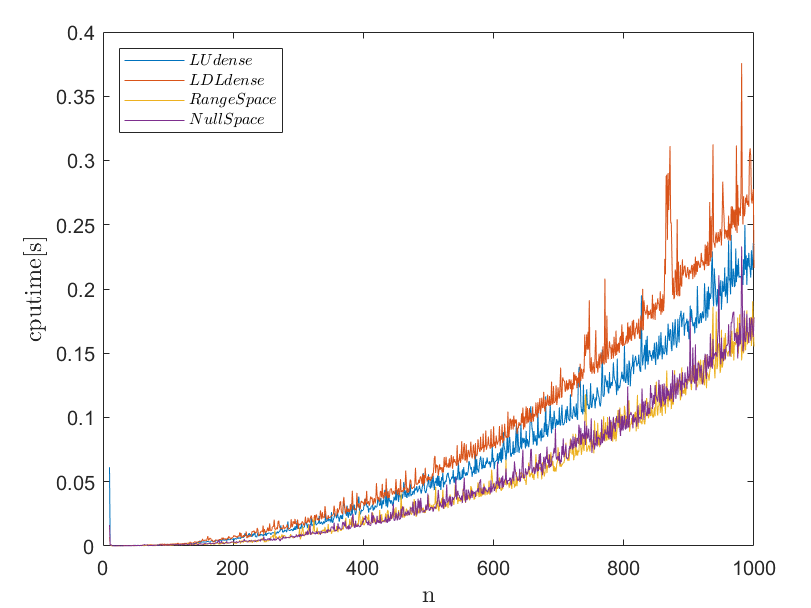
\includegraphics[scale=0.7]{figures/EQ_NOSPARSE.PNG}
\caption{CPU time of LU-dense, LDL-dense, range-space, and null-space}
\label{fig:labe1.4.1}
\end{figure}
It is found that with the increase in the number of variables, the CPU time required by the four factorization is gradually increasing. Compared with LU-factorization (dense) and LDL-factorization (dense), range-space factorization and null-space factorization take less CPU time and maintain almost the same performance. LU and LDL require the same CPU time when the number of variables is small, but as the number of variables increases, the difference between the CPU time required for LDL and LU gradually increases.\\
Then the CPU time of LU-factorization (sparse) and LDL-factorization (sparse) is test. The curve of CPU time of these LU-dense, LU-sparse, LDL-dense and LDL-sparse is showed
\begin{figure}[H]
\centering
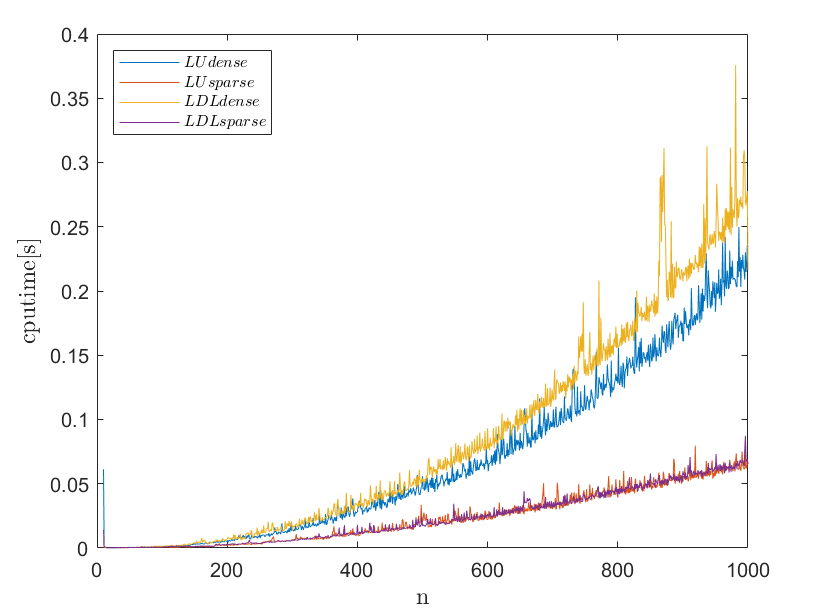
\includegraphics[scale=0.7]{figures/EQ_KKT_LULDL.PNG}
\caption{CPU time of LU-dense, LU-sparse, LDL-dense and LDL-sparse}
\label{fig:labe1.4.2}
\end{figure}
It is found that both the sparse factorization of LU and LDL significantly reduce CPU time compared to their respective dense factorization, and maintain similar performance.\\
The CPU time curves of all methods are shown here
\begin{figure}[H]
\centering
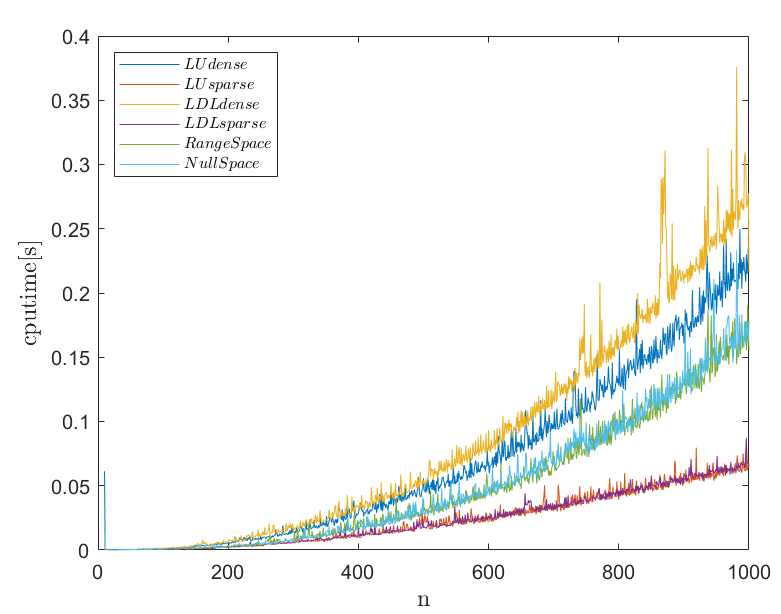
\includegraphics[scale=0.7]{figures/EQ_ALL.PNG}
\caption{CPU time of LU-dense, LU-sparse, LDL-dense, LDL-sparse, range-space, and null-space}
\label{fig:labe1.4.3}
\end{figure}
It can be seen that the sparse method factorization LDL and LU requires the least CPU time, and can maintain a CPU time of less than 0.1s when the KKT matrix is $1000 \times 1000$, while range-space factorization and null-space factorization need to be less than about 0.2s, and the dense factorization of LU requires less than 0.25s, and the dense factorization of LDL takes the most CPU time, which takes about 0.3s.
\newpage
\section{ \bfseries Quadratic Program (QP)}
The quadratic program (QP) is considered in the form (assume that $A$ has full column rank)\\
\begin{align*}
&\min_{x} \quad \phi=\frac{1}{2} x^{\prime} H x+g^{\prime} x \tag{2}\label{con:op2}\\
& s.t. \quad A^{\prime} x=b\\
& \quad \quad  l\le x \le u
\end{align*}
%%%%%%%%%%%%%%%%%%%%%%%%%%%%%%%%%%%%%%%%%%
%%%%%%%%%%%%%%%%%%%%%%%%%%%%%%%%%%%%%%%%%%%%%%%%%%%%%%%%%%%%%%%%%%%%%%%%%%%%%%%%%%%%%
%%%%%%%%%%%%%%%%%%%%%%%%%%%%%%%%%%%%%%%%%%%
%%%%%%%%%%%%%%%%%%%%%%%%%%%%%%%%%%%%%%%%%%
%%%%%%%%%%%%%%%%%%%%%%%%%%%%%%%%%%%%%%%%%%%
\subsection{\bfseries Lagrangian function}
\begin{shaded}
{ Question: What is the Lagrangian function for this problem?}
\end{shaded}
The quadratic program problem (\ref{con:op2}) can be equivalent to the inequailty constrained form
\begin{align*}
&\min_{x} \quad \phi=\frac{1}{2} x^{\prime} H x+g^{\prime} x \tag{2.1}\label{con:op2.1}\\
& s.t. \quad A^{\prime} x=b\\
& \quad \quad  c(x)=\begin{bmatrix}
x-l \\ u-x\end{bmatrix}=\left[I\quad -I\right]^{\prime}x+\begin{bmatrix}
-l \\ u\end{bmatrix}\ge 0\Leftrightarrow C^{\prime}x \ge d
\end{align*}
Lagrangian function\\
$$L(x,y,z)=\frac{1}{2}x^{\prime}Hx+g^{\prime}x-y^{\prime}\left(A^{\prime}x-b\right)-z^{\prime}\left(C^{\prime}x-d\right)\eqno{(2.2)}$$
%%%%%%%%%%%%%%%%%%%%%%%%%%%%%%%%%%%%%%%%%%
%%%%%%%%%%%%%%%%%%%%%%%%%%%%%%%%%%%%%%%%%%%
%%%%%%%%%%%%%%%%%%%%%%%%%%%%%%%%%%%%%%%%%%
%%%%%%%%%%%%%%%%%%%%%%%%%%%%%%%%%%%%%%%%%%%
%%%%%%%%%%%%%%%%%%%%%%%%%%%%%%%%%%%%%%%%%%
%%%%%%%%%%%%%%%%%%%%%%%%%%%%%%%%%%%%%%%%%%%
\subsection{\bfseries Optimality conditions}
\begin{shaded}
{Question: Write the nesessary and sufficient optimality conditions for this problem.}
\end{shaded}
\begin{align*}
& \nabla_{x} L\left(x,y,z\right)=Hx+g-Ay-Cz=0\tag{2.3}\\
& \nabla_{y} L\left(x,y,z\right)=-\left(A^{\prime}x-b\right)=0\tag{2.4}\\
& \nabla_{z} L\left(x,y,z\right)=-\left(C^{\prime}x-d\right) \le 0\tag{2.5}\\
& z \ge 0 \tag{2.6}\\
& \left(C^{\prime}x-d\right)_iz_i=0 \quad i=1,2,...,m_c \tag{2.7}
\end{align*}
%%%%%%%%%%%%%%%%%%%%%%%%%%%%%%%%%%%%%%%%%%
%%%%%%%%%%%%%%%%%%%%%%%%%%%%%%%%%%%%%%%%%%%
%%%%%%%%%%%%%%%%%%%%%%%%%%%%%%%%%%%%%%%%%%
%%%%%%%%%%%%%%%%%%%%%%%%%%%%%%%%%%%%%%%%%%%
%%%%%%%%%%%%%%%%%%%%%%%%%%%%%%%%%%%%%%%%%%
%%%%%%%%%%%%%%%%%%%%%%%%%%%%%%%%%%%%%%%%%%%
\subsection{\bfseries Primal-dual interior-point algorithm}
\begin{shaded}
{Question: Write pseudo-code for a primal-dual interior-point algorithm for solution of this
problem. Explain each major step in your algorithm.}
\end{shaded}
{\setmainfont{Times New Roman}\bfseries Pseudo-code}
\begin{algorithm}[!h]
	\caption{Primal-Dual Predictor-Corrector Interior-Point Algorithm}
	\begin{algorithmic}[1]
	    \STATE Given an input $H$, $g$, $A$, $b$, $C$, $d$ and compute the starting point $x_0$, $y_0$, $z_0$, $s_0$ with ($z_0$,$s_0$)>0\\
		\STATE Compute the residuals $r_L$, $r_A$, $r_C$, $r_{sz}$ and duailty gap $\mu$\\
		\STATE Check convergence conditions\\
		
        \WHILE {(not converged)}\\
		\STATE Compute the affine step direction $\Delta x^{aff}$, $\Delta z^{aff}$ and $\Delta s^{aff}$\\
		\STATE Compute the affine step size $\alpha ^{aff}$\\
		\STATE Compute the affine duality gap $\mu ^{aff} $\\
		\STATE Compute centering parameter $\sigma$\\
		\STATE Compute affine-centering-correction direction\\
		\STATE Compute the step size $\alpha * \eta$ and update the iteration of $x$, $y$, $z$ and $s$ to take the actual step\\
		\STATE Re-compute the residuals $r_L$, $r_A$, $r_C$, $r_{sz}$ and duailty gap $\mu$\\
		\STATE Check convergence conditions and stop if it converged\\
		\ENDWHILE
    \end{algorithmic}
\end{algorithm}

The inequality in the form of this problem requires further introduction of slack variables
$$s \triangleq C^{\prime} x-d \ge 0\eqno{(2.8)}$$
implies
\begin{align*}
& -C^{\prime}x+s+d=0\tag{2.9}\\
& s \ge 0
\end{align*}
The optimality conditions can be expressed as
\begin{align*}
& r_L=Hx+g-Ay-Cz=0\tag{2.10}\\
& r_A=-\left(A^{\prime}x-b\right)=0\tag{2.11}\\
& r_C=-\left(C^{\prime}x-d\right) \ge 0\tag{2.12}\\
& r_{SZ}=SZe=0\tag{2.13}\\
& s \ge 0, \quad z \ge 0\tag{2.14}
\end{align*}

Several enhancements have a significant effect on practical performance, so the Primal-dual interior-point algorithm implemented here is based on Mehrotra's predictor-corrector method. \\[0.3cm]
In the first step, a set of feasible starting point needs to be computed. A heuristic\cite{NoceWrig06} for starting point on p.484 in Nocedal \& Wright is introduced.
\begin{algorithm}[H]
	\caption{Heuristic for an starting point}
	\begin{algorithmic}[1]
	    \STATE Given an input $\bar{x}$, $\bar{y}$, $\bar{z}$, $\bar{s}$ with ($\bar{z}$,$\bar{s}$)>0\\
		\STATE Compute the residuals $r_L$, $r_A$, $r_C$ and  $r_{sz}$\\
		\STATE Compute affine search direction from $\bar{x}$, $\bar{y}$, $\bar{z}$ and $\bar{s}$\\
		\STATE $x=\bar{x}$, $y=\bar{y}$, $z=max\{1,|\bar{z}+\Delta z^{aff}|\}$, $s=max\{1,|\bar{s}+\Delta s^{aff}|\}$
    \end{algorithmic}
\end{algorithm}
The Primal-dual interior-point algorithm is based on iterative calculation. And the strict positivity of $z$ and $s$ is maintained throughout and each step is a Newton-like step involving a centering component. Therefore, in fact, the Primal-dual interior-point algorithm uses a less aggressive Newton direction, which is to control the iteration point so that it gradually approaches the constraint boundary and the optimal solution. The specific method is that when the Newton method is used to solve a nonlinear system, it is not required to directly achieve $r_{SZ}=SZe=0$ in each iteration, but to make it equal to a gradually decreasing value, which is $r_{SZ}=SZe=\sigma \mu e$, where $\mu$ is the current duailty gap, and $\sigma \in [0,1]$ is the center parameter used to control the descent speed.\\
The specific steps of iteration are: An affine step is computed. 
$$\left[\begin{array}{cccc}
H & -A & -C & 0 \\
-A^{\prime} & 0 & 0 & 0 \\
-C^{\prime} & 0 & 0 & I \\
0 & 0 & S & Z
\end{array}\right]\left[\begin{array}{l}
\Delta x^{a f f} \\
\Delta y^{a f f} \\
\Delta z^{a f f} \\
\Delta s^{a f f}
\end{array}\right]=\left[\begin{array}{c}
-r_{L} \\
-r_{A} \\
-r_{C} \\
-r_{S Z}
\end{array}\right]\eqno{(2.15)}$$
Then the center parameter $\sigma$ will be made small if the affine step is good, or to be set as 1 if the affine step is bad, by which the iteration point can stay close to central path. So $\alpha^{aff}$ is defined as the largest value satisfying
\begin{align*}
&z+\alpha^{a f f} \Delta z^{a f f} \geq 0\tag{2.16}\\
&s+\alpha^{a f f} \Delta s^{a f f} \geq 0\tag{2.17}
\end{align*}
Then Duality gap $\mu_{aff}$ is defined for affine step
$$\mu^{a f f}=\frac{\left(z+\alpha^{a f f} \Delta z^{a f f}\right)^{\prime}\left(s+\alpha^{a f f} s^{a f f}\right)}{m_{c}}\eqno{(2.18)}$$
The centering parameter is calculated as a heuristic
$$\sigma=\left(\frac{\mu^{a f f}}{\mu}\right)^{3} \quad with \quad \mu=\frac{z^{\prime} s}{m_{c}}\eqno{(2.19)}$$
Then affine-centering-correction direction is computed by solving
$$\left[\begin{array}{cccc}
H & -A & -C & 0 \\
-A^{\prime} & 0 & 0 & 0 \\
-C^{\prime} & 0 & 0 & I \\
0 & 0 & S & Z
\end{array}\right]\left[\begin{array}{c}
\Delta x \\
\Delta y \\
\Delta z \\
\Delta s
\end{array}\right]=-\left[\begin{array}{c}
r_{L} \\
r_{A} \\
r_{C} \\
r_{S Z}+\Delta S^{a f f} \Delta Z^{a f f} e-\sigma \mu e
\end{array}\right]\eqno{(2.20)}$$
Update
$$\left[\begin{array}{l}
x \\
y \\
z \\
s
\end{array}\right]=\left[\begin{array}{l}
x+\eta \alpha \Delta x \\
y+\eta \alpha \Delta y \\
z+\eta \alpha \Delta z \\
s+\eta \alpha \Delta s
\end{array}\right]\eqno{(2.21)}$$
Finally the residuals are recomputed and convergence is defined as situation that the residuals $r_L$, $r_A$, $r_C$ and  $r_{SZ}$ are all below a given small value $\epsilon$.
%%%%%%%%%%%%%%%%%%%%%%%%%%%%%%%%%%%%%%%%%%
%%%%%%%%%%%%%%%%%%%%%%%%%%%%%%%%%%%%%%%%%%%
%%%%%%%%%%%%%%%%%%%%%%%%%%%%%%%%%%%%%%%%%%
%%%%%%%%%%%%%%%%%%%%%%%%%%%%%%%%%%%%%%%%%%%
%%%%%%%%%%%%%%%%%%%%%%%%%%%%%%%%%%%%%%%%%%
%%%%%%%%%%%%%%%%%%%%%%%%%%%%%%%%%%%%%%%%%%%
\newpage
\subsection{\bfseries Primal-dual interior-point algorithm implementation}
\begin{shaded}
{Question: Implement the primal-dual interior-point algorithm and test it. You must provide commented code as well as driver files to test your code, documentation that it works, and performance statistics.}
\end{shaded}
The matlab code of Primal-dual interior-point algorithm is showed here\\

{\setmainfont{Courier New Bold} \scriptsize            
\begin{lstlisting}
function [x,output]=PD_ipQP(H,g,A,b,C,d,x0,y0,z0,s0)
% PD_ipQP   Primal-dual interior-point algorithm
%
%          min  0.5*x'*H*x+g'*x
%           x
%          s.t. A x  = b      
%               C x >= d      
%         rL = Hx + g − Ay − Cz = 0 
%         rA = −Ax + b = 0 (Lagrange multiplier y)
%         rC = −Cx + s + d = 0 (Lagrange multiplier z)
%         s ≥ 0 (Slack variables )
%         sz = 0
% Syntax: [x,output]=PD_ipQP(H,g,A,b,C,d,x0,y0,z0,s0)
%         output.fval: minimum value
%         output.y: final y
%         output.s: final s
%         output.z: final z
%         output.Xarray: Iteration trajectory  
          
iteration_max=50;
epsilon=1.0e-9;
eta=0.995;
noeq=0;
Xarray=[];
Xarray=[Xarray x0];
nh=size(H,1);%dimension of x
na=size(A,2);%A'x=b
nc=size(C,2);%C'x>=d
e=ones(nc,1);
%residual
S0=diag(s0);
Z0=diag(z0);
%if no equlity equations
if isempty(A)&isempty(b)
    noeq=1;
end

if  noeq==1
    rL=H*x0+g-C*z0;
    rA=0.*x0;
    rC=s0+d-C'*x0;
    rsz=S0*Z0*e;
else
    rL=H*x0+g-A*y0-C*z0;
    rA=b-A'*x0;
    rC=s0+d-C'*x0;
    rsz=S0*Z0*e;
end

%duality gap
mu=(z0'*s0)/nc;

stop_flag=0;
iteration=0;
x=x0;
y=y0;
S=S0;
Z=Z0;
while(~stop_flag&iteration<=iteration_max)
    
    H_bar=H+C*(inv(S)*Z)*C';
    if noeq==1
     KKT=H_bar;
    else
    KKT=[H_bar -A;-A' zeros(na,na)];
    end
    
    [L, D, p] = ldl(KKT, 'lower', 'vector');
    %Affine Direction
    rL_bar=rL-C*(inv(S)*Z)*(rC-inv(Z)*rsz);
    if noeq==1
        KKT_b=-rL_bar;
    else
    KKT_b=-[rL_bar;rA];
    end
    delta_xy=zeros(size(KKT_b,1),1);
    delta_xy(p) = L'\(D\(L\KKT_b(p)));
    delta_x=delta_xy(1:nh);
    delta_z=-(inv(S)*Z)*C'*delta_x+(inv(S)*Z)*(rC-inv(Z)*rsz);
    delta_s=-inv(Z)*rsz-inv(Z)*S*delta_z;
    
    %compute the lagest alf
    z=diag(Z);
    s=diag(S);
    delta_zs=[delta_z;delta_s];
    alf_c=-[z;s]./delta_zs;
    alf_aff=min([1;alf_c(delta_zs<0)]);
    
    %compute the affine duality gap
    mu_aff=(z+alf_aff*delta_z)'*(s+alf_aff*delta_s)/nc;
    %compute the centering parameter
    sigma=(mu_aff/mu)^3;
    
    %Affine-Centering-Correction Direction
    delta_S=diag(delta_s);
    delta_Z=diag(delta_z);
    rsz_bar=rsz+delta_S*delta_Z*e-sigma*mu*e;
    %update Affine Direction
    rL_bar=rL-C*(inv(S)*Z)*(rC-inv(Z)*rsz_bar);
    if noeq==1
        KKT_b=-rL_bar;
    else
    KKT_b=-[rL_bar;rA];
    end
    delta_xy=zeros(size(KKT_b,1),1);
    delta_xy(p) = L'\(D\(L\KKT_b(p)));
    delta_x=delta_xy(1:nh);
    delta_y=delta_xy(nh+1:end);
    delta_z=-(inv(S)*Z)*C'*delta_x+(inv(S)*Z)*(rC-inv(Z)*rsz_bar);
    delta_s=-inv(Z)*rsz_bar-inv(Z)*S*delta_z;
    %update alf
    delta_zs=[delta_z;delta_s];
    alf_c=-[z;s]./delta_zs;
    alf_aff=min([1;alf_c(delta_zs<0)]);
    alf_bar=alf_aff*eta;
    %compute new state
    x=x+alf_bar*delta_x;
    y=y+alf_bar*delta_y;
    z=z+alf_bar*delta_z;
    s=s+alf_bar*delta_s;
    Z=diag(z);
    S=diag(s);
    %compute residuals
    if noeq==1
        rL=H*x+g-C*z;
        rA=0.*x;
        rC=s+d-C'*x;
        rsz=S*Z*e;
    else
        rL=H*x+g-A*y-C*z;
        rA=b-A'*x;
        rC=s+d-C'*x;
        rsz=S*Z*e;
    end
    mu=z'*s/nc;
    %stop judge
    judge = [norm(rL,1), norm(rA,1), norm(rC,1), abs(mu)];
    stop_flag = (length(judge(judge < epsilon)) == 4);
    Xarray=[Xarray x];
    iteration=iteration+1;
end
fval=0.5*x'*H*x+g'*x;
output.fval=fval;
output.y=y;
output.s=s;
output.z=z;
output.Xarray=Xarray;
output.iteration=iteration;
end
\end{lstlisting}}

In the later section on the comparison of the two algorithms, the test of the algorithm with a test problem that can be randomly generated and control the size of the variable is carried out. Here is just a simple verification of the feasibility of the algorithm.\\
Two problems that meet the format requirements are used to test the implemented algorithm, a quadratic programming problem with equality constraints and a quadratic programming problem with only inequality constraints($A=0, b=0$)\\
\begin{align*}
    &\min_{x}\quad \phi(x)=\left(x_1-1\right)^2+\left(x_2-2.5\right)^2 \tag{2.22}\\
    &\text{s.t.} \quad x_1-x_2= 1   \qquad \qquad -1<x_1<2\\
    &\quad \quad -1<x_1<2 \qquad \qquad -1<x_2<2\\
    &\quad \quad -1<x_2<2\\
    &\quad \qquad \text{problem1} \qquad \qquad \qquad \text{problem2}
\end{align*}\\
Four starting points are chose to check the result of the problem1 and problem2 respectively, $A(-1,4)$ and $B(4,-1)$ which located outside the feasible area, $C(1,-1)$ which located at the edge of the inequailty constraint, and $D(0,0)$ which located inside the feasible area. First $H$ and $g$ of the objective function which will be used in the test are calculated
$$H=\begin{bmatrix}
2&0\\
0&2
\end{bmatrix} \qquad 
g=\begin{bmatrix}
-2\\
-5
\end{bmatrix}$$
The driver files are stated in the appendix \ref{6.2.1} and \ref{6.2.2}. The iterative trajectory in the contour for the problem1 is showed here
\vspace{-0.3cm}
\begin{figure}[H]
\centering
\setlength{\abovecaptionskip}{-0.2cm} 
\setlength{\belowcaptionskip}{-0.5cm} 
\subfigure[$A(-1,4)$]{
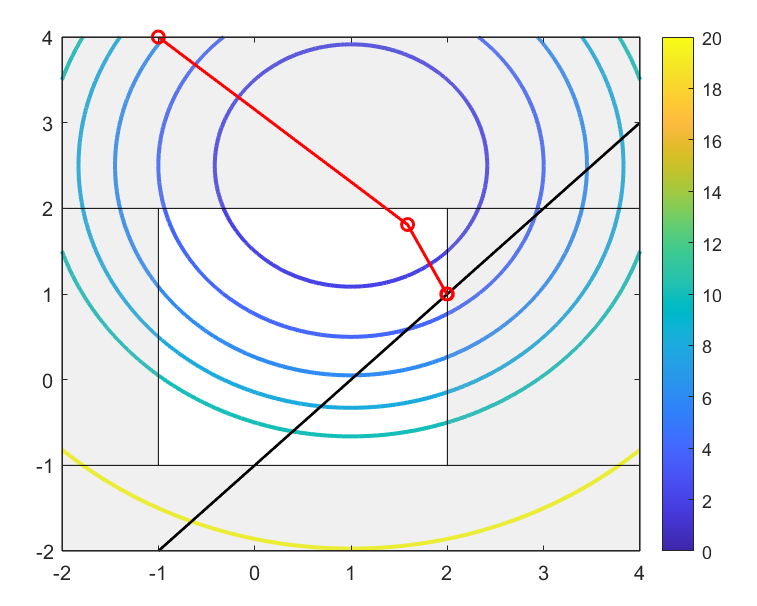
\includegraphics[scale=0.35]{figures/QP_IP_1_A.PNG}
%\caption{fig1}
}
\quad
\subfigure[$B(4,-1)$]{
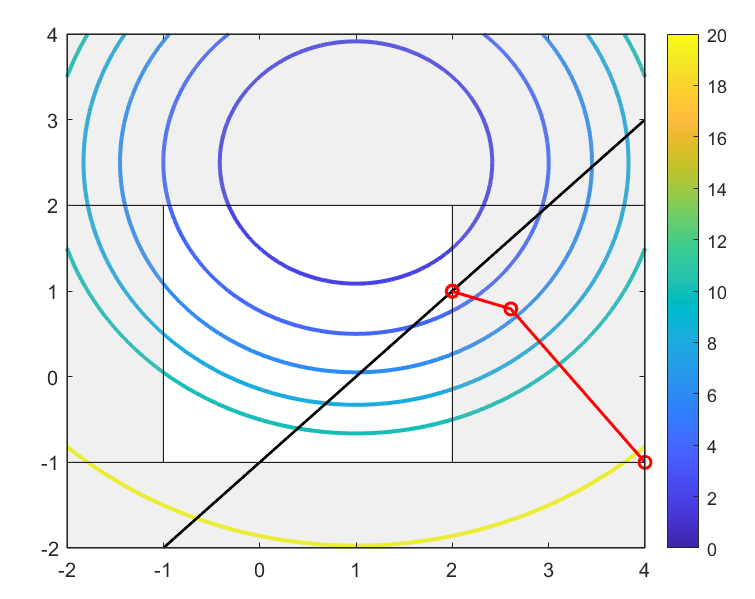
\includegraphics[scale=0.35]{figures/QP_IP_1_B.PNG}
}
\quad
\subfigure[$C(1,-1)$]{
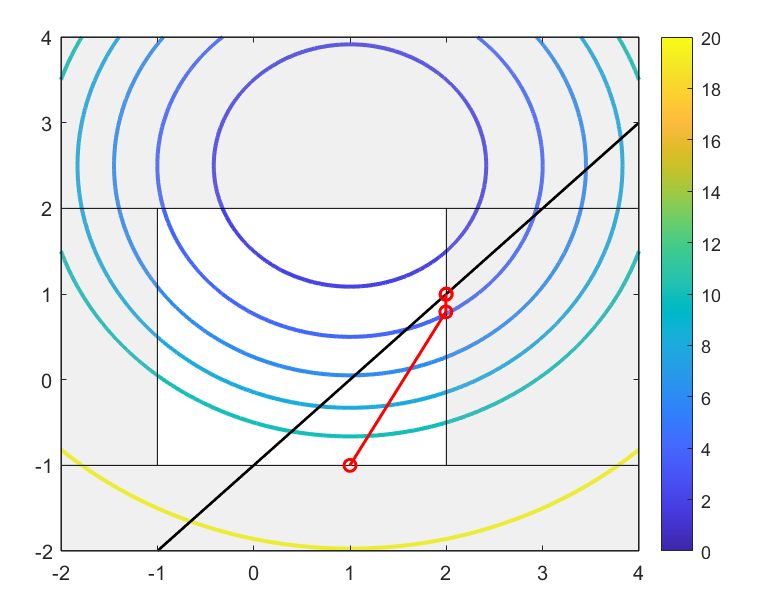
\includegraphics[scale=0.35]{figures/QP_IP_1_C.PNG}
}
\quad
\subfigure[$D(0,0)$]{
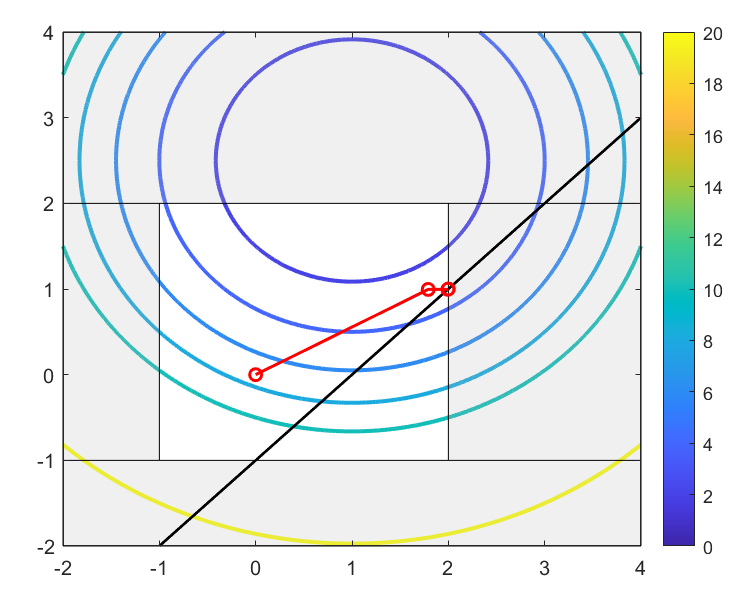
\includegraphics[scale=0.35]{figures/QP_IP_1_D.PNG}
}
\caption{ Iterative trajectory in contour of problem1}

\end{figure}
It can be seen that in the test of Problem 1, the four starting  points all reached the minimum point under the equality and inequality constraints with a small number of iterations.\\
Then the iterative trajectory in the contour for the problem2 is showed 
\vspace{-0.3cm}
\begin{figure}[H]
\centering
\setlength{\abovecaptionskip}{-0.2cm} 
\setlength{\belowcaptionskip}{-0.5cm} 
\subfigure[$A(-1,4)$]{
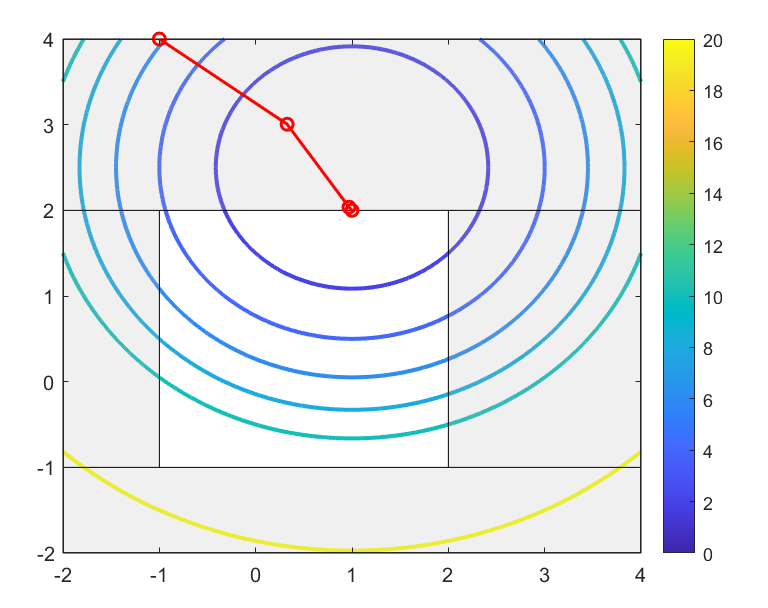
\includegraphics[scale=0.35]{figures/QP_IP_2_A.PNG}
%\caption{fig1}
}
\quad
\subfigure[$B(4,-1)$]{
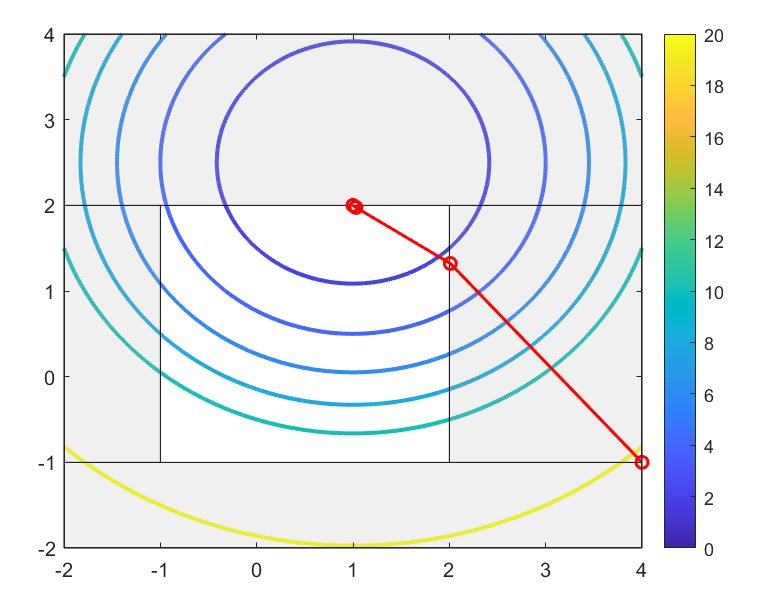
\includegraphics[scale=0.35]{figures/QP_IP_2_B.PNG}
}
\quad
\subfigure[$C(1,-1)$]{
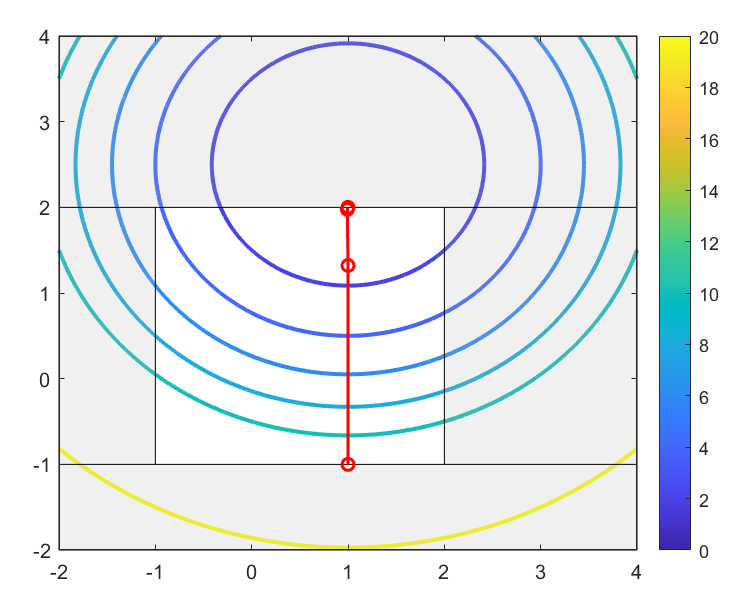
\includegraphics[scale=0.35]{figures/QP_IP_2_C.PNG}
}
\quad
\subfigure[$D(0,0)$]{
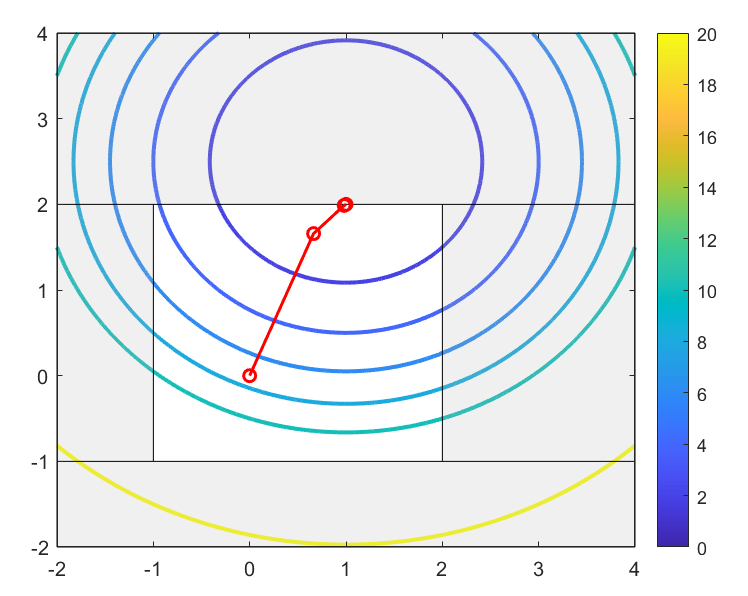
\includegraphics[scale=0.35]{figures/QP_IP_2_D.PNG}
}
\caption{ Iterative trajectory in contour of problem2}
\end{figure}

Also in the test of Problem 2, the four initial points all reached the minimum point under the constraint of inequality with a small number of iterations
%%%%%%%%%%%%%%%%%%%%%%%%%%%%%%%%%%%%%%%%%%
%%%%%%%%%%%%%%%%%%%%%%%%%%%%%%%%%%%%%%%%%%%
%%%%%%%%%%%%%%%%%%%%%%%%%%%%%%%%%%%%%%%%%%
%%%%%%%%%%%%%%%%%%%%%%%%%%%%%%%%%%%%%%%%%%%
%%%%%%%%%%%%%%%%%%%%%%%%%%%%%%%%%%%%%%%%%%
%%%%%%%%%%%%%%%%%%%%%%%%%%%%%%%%%%%%%%%%%%%
\subsection{\bfseries Primal Active-Set Algorithm}
\begin{shaded}
{Question: Write pseudo-code for a primal active-set algorithm. Explain the algorithm.}
\end{shaded}
\begin{algorithm}[H]
	\caption{Primal Active-Set Algorithm}
	\begin{algorithmic}[1]
	    \STATE Compute a feasible starting point $x_0$\\
		\STATE Let $W_0$ be the corresponding active set: $A_0=\{ i:a_i^{\prime}x_0=b_i \}$\\
		\WHILE {(not stop)}\\
		\STATE Solve a quadratic subproblem to find $p_k$\\
		\IF{($p_k=0$)}\\
		\IF{($\lambda_{i} \geq 0, \forall i \in W_{k} \cap I$)}\\
		\STATE The optimal solution has been found\\
		\STATE break\\
		\ELSE\\
		\STATE Let $j \in W_k$ be an index such that $\lambda_i<0$, Remove constraint $j$ from the working set. $W_{k+1}=W_k \backslash \{j\}$\\
		\ENDIF\\
		\ELSE\\
		\STATE Compute the distance $\alpha$ to the nearest inactive constraint in the search direction\\
		\IF{($\alpha < 1$)}\\
		\STATE $x_{k+1}=x_k+\alpha p_K$, add constraint $j$ to the working set. $W_{k+1}=W_k \cap \{ j \}$\\
		\ELSE\\
		\STATE $x_{k+1}=x_k+ p_K$, $W_{k+1}=W_k$\\
		\ENDIF\\
		\ENDIF\\
		\ENDWHILE
    \end{algorithmic}
\end{algorithm}

Similar to the characteristics of the simplex method of linear programming, both the Active-set method and the simplex method are to iterate the point and follow the constraint boundary until the optimal solution is reached. But Active-set methods form QP differ from the simplex method in that the iterates(and the solution $x^*$) are not necessarily vertices of the feasible region.\\[0.3cm]
In the first step, a set of feasible starting point needs to be computed. Here a "Phase I" method \cite{NoceWrig06} is introduced for active set algorithm. Given $\tilde{x}$ of the vector $x$, the following feasibility linear program is defined
$$\begin{array}{ll}
\min _{x, z} \quad e^{T} z \\
\text {s.t.} \qquad a_{I}^{T} x+\gamma_{i} z_{i}=b_{i} & i \in \mathcal{E} \\
\qquad  \quad a_{I}^{T} x+\gamma_{i} z_{i} \geq b_{i} & i \in \mathcal{I} \\
\qquad \quad x \in X & \\
\qquad \quad z \geq 0
\end{array}\eqno{(2.23)}$$
Where $e=(1,1,...,1)^T$, $\gamma_i=-sign\left(a_i^T\tilde{x}-b_i\right)$ for $i\in\mathcal{E} $,and $\gamma_i=1$ for $i\in\mathcal{I} $. If the initial guess is feasible then the solution to the above problem will be $(\tilde{x}, 0)$.
Primal active-set methods find a step from one iterate to the next by solving a quadratic subproblem as stated in step 2 in which some of the inequality constraints, and all the equality constraints, are imposed as equalities. This subset is referred to as the working set and is denoted at the $k$th iterate $x_k$ by $W_k$.
One important thing that need to be satisfied is the strict linear independent property of the gradients $a_i$ of the constraints in the working set $W$.
As the starting point computed, in order to check whether $x_k$ minimizes the quadratic $\phi$ in the subspace defined by the working set $W_k$, A step $p$ needs to be computed by solving an equality-constrained QP sub-problem in which the constraints corresponding
to the working set $W_k$ are regarded as equalities and all other constraints are temporarily disregarded.\\
\begin{align*}
&\min _{p}\quad \frac{1}{2} p^{\prime} G p+\left(G x_{k}+g\right)^{\prime} p \tag{2.24}\\
&s.t. \quad a_{i}^{\prime} p=0 \quad i \in \mathcal{W}_{k}
\end{align*}
Assuming that the optimal $p_k$ is nonzero, it is necessary to decide how far to move along this direction. If $x_k + p_k$ is feasible for all the constraints of the original problem, then $\alpha_k = 1$, otherwise $\alpha_k$ is a positive number less than 1. The step length $\alpha$ is defined and a new iterate is obtained
$$x_{k+1}=x_k+\alpha_kp_k\eqno{(2.25)}$$
Regarding the calculation of the step size $\alpha_k$,  the calculation of the step size is mainly to ensure that the new iteration point does not violate the constraints of the original problem. Since the constraints $i \in W_k$ are satisfied, the constraints that are not in the work set are only focused. The first step is to judge the sign of $a_i^{T}p_k$. If $a_i^{T}p_k>0$, then the analysis shows that as long as the step size $\alpha>0$0, the constraint must be satisfied, so the main concerns needed to pay attention to are those constraints with $a_i^{T}p_k<0$.\\
$$\alpha_{k}=\min \left(1, \min _{i \notin \mathcal{W}_{k}, a_{i} T_{k}<0} \frac{b_{i}-a_{i}^{T} x_{k}}{a_{i}^{T} p_{k}}\right)\eqno{(2.26)}$$
 Through the above method,the effective constraints can be continued to add to the working set until it is found that the current iteration point is the optimal solution of the current working set in a certain iteration, that is $p_k=0$ calculated at this time. Next step is to verify whether the current iteration point is the optimal solution of the original problem. The method of verification is to determine whether the Lagrange multipliers $\lambda$ corresponding to the constraints in the working set are all greater than or equal to 0. If so, the iteration is exited and the optimal solution of the original problem is given.\\
 $$\sum_{i \in \hat{w}} a_{i} \hat{\lambda}_{i}=g=G \hat{x}+c\eqno{(2.27)}$$
 If there are one or more calculated $\hat{\lambda}_{i}<0$. Then it shows that by removing one or more constraints of the working set, the value of the objective function can be further reduced. Therefore, one of the constraints with the corresponding $\hat{\lambda}_{i}<0$ will be selected, and removed from the working set $W_k$ to construct a new working set $W_{k+1}$. If there is more than one optional constraint, the constraint corresponding to the minimum (maximum absolute value) of $\hat{\lambda}_{i}$ will be removed.
 \newpage
 %%%%%%%%%%%%%%%%%%%%%%%%%%%%%%%%%%%%%%%%%%%%%%%%%%%%%%%%%%%%%%%%%%%%%%%%%%%%%%%%%%%%%%%%%%%%%%%%%%%%%%%%%%%%%%%%%%%%%%%%%%%%%%%%%%%%%%%%%%%%%%%%%%%%%%%%%%%%%%%%%%%%%%%%%%%%%%%%%%%%%%%%%%%%%%%%%%%%%%%%%%%%%%%%%%%%%%%%%%%%%%%%%%%%%%%%%%%%%%%%%%%%%%%%%%%%%%%%%%%%%%%%
 \subsection{\bfseries Primal Active-Set Algorithm implementation}
\begin{shaded}
{Question: Implement the primal active-set algorithm and test it. You must provide commented code as well as driver files to test your code, documentation that it works,
and performance statistics}
\end{shaded}

The main matlab code of Primal Active-Set Algorithm is showed here, and the function "As\_sub" which solve the sub-problem is stated in appendix \ref{6.2.3}.

{\setmainfont{Courier New Bold} \scriptsize            
\begin{lstlisting}
function [x,lam,exitflag,output]=Pri_AsQp(H,g,Ae,be,Ai,bi,x0)
% Pri_AsQp   Primal Active-Set Algorithm
%
%          min  0.5*H'*x*H+g'*x
%           x
%          s.t. Ae x  = be      
%               Ai x >= bi      
%
% Syntax: [x,lam,exitflag,output]=Pri_AsQp(H,g,Ae,be,Ai,bi,x0)
%         output.lam: Lagrange multiplier
%         output.x_plot: Iteration trajectory              
%Initialization
%Ax>=b;
epsilon=1.0e-9;
err=1.0e-6;
iteration=0;
x=x0;
n=length(x);
iteration_max=20;
ne=length(be);
ni=length(bi);
lam=zeros(ne+ni,1);
index=ones(ni,1);
output.x_plot=[x0'];
output.lam=[lam'];

%initialize the active set(index=1)
for(i=1:ni)
    if(Ai(i,:)*x>bi(i)+epsilon)
        index(i)=0;
    end
end
%main program
while(iteration<=iteration_max)
    
    Aee=[];
% if the start point x is on the Equality Constraint or on the edge of the
% Equality Constraint, put it in active set.
    if(ne>0)
        Aee=Ae;
    end
    for j=1:ni
        if(index(j)>0)
            Aee=[Aee;Ai(j,:)];
        end
    end
    %Solve subproblem to find p and Compute Lagrange multipliers
    gk=H*x+g;
    [m1,n1]=size(Aee);
    [p,lam]=As_sub(H,gk,Aee,zeros(m1,1));
    if(norm(p)<=err)
        lambda_min=0.0;
        if(length(lam)>ne)
            [lambda_min,jk]=min(lam(ne+1:end));
        end
        if(lambda_min>=0)
            exitflag=1;
        else
            exitflag=0;
            %remove the (Lagrange multipliers min) inequlity Constraint
            %form active set
            for(i=1:ni)
                if(index(i)&(sum(index(1:i)))==jk)
                    index(i)=0;
                    break;
                end
            end
        end
        iteration=iteration+1;
    else
        exitflag=0;
        %computer the step length
        alpha=1.0;
        tm=1.0;
        for(i=1:ni)
            if((index(i)==0)&(Ai(i,:)*p<0))
                tm1=(bi(i)-Ai(i,:)*x)/(Ai(i,:)*p);
                if(tm1<tm)
                    tm=tm1;
                    ti=i;
                end
            end
        end
        
        alpha=min(alpha,tm);
        x=x+alpha*p;
        %update the active set
        if(tm<1)
            index(ti)=1;
        end
    end
    if(exitflag==1)
        break;
    end
    iteration=iteration+1;
    output.x_plot=[output.x_plot;x'];
    if(length(lam)<(ne+ni))
        lam=[lam;zeros(ne+ni-length(lam),1)];
    end
    output.lam=[output.lam;lam'];
end
output.fval=0.5*x'*H*x+g'*x;
output.iter=iteration;
\end{lstlisting}}
In the later chapter on the comparison of the two algorithms, an algorithm with a test problem that can be randomly generated and control the size of the variable will be test. Here is just a simple verification of the feasibility of the algorithm.\\
The same two problems tested by Primal-dual interior-point algorithm in section 2.4 are used. However, the different starting points for active-set algorithm should be chose because the iteration of active-set method can only be implemented in the feasible region. And for quadratic problem which has equality constraints, the starting points have to be located at the equality constraints. So we choose starting points $A_1(0,-1)$ and $B_1(1,0)$ for the problem2, and starting points $A_2(0,-1)$, $B_2(2,0)$, $C_2(0,2)$ and $D_2(-1,0)$ for the problem2.\\[0.3cm]
The driver files are stated in the appendix \ref{6.2.4} and \ref{6.2.5}. The iterative trajectory in the contour for the problem1 is showed here
\begin{figure}[H]
\centering
\subfigure[$A(0,-1)$]{
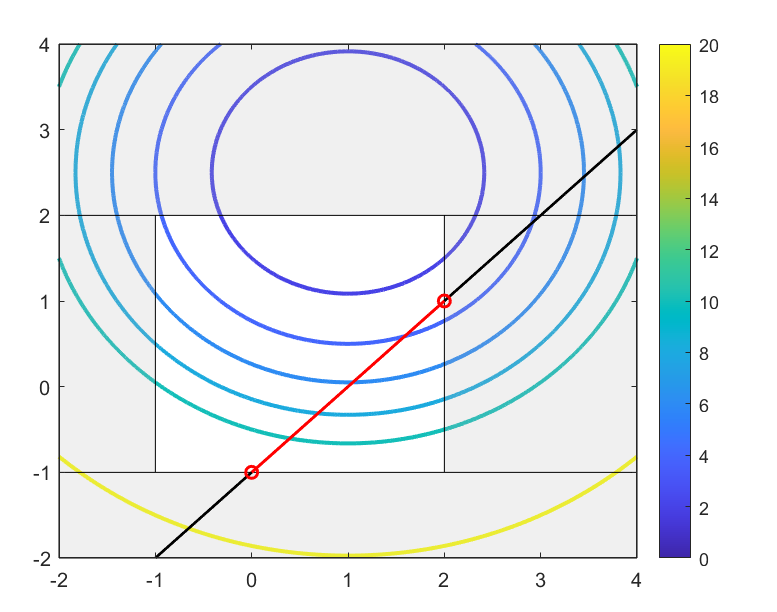
\includegraphics[scale=0.4]{figures/QP_AS_1_A.PNG}
%\caption{fig1}
}
\quad
\subfigure[$B(1,0)$]{
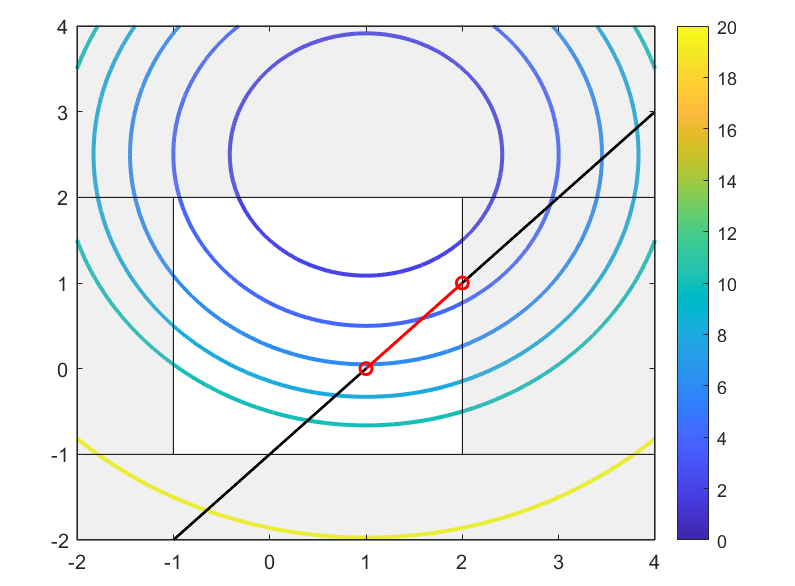
\includegraphics[scale=0.4]{figures/QP_AS_1_B.PNG}
}
\caption{ Iterative trajectory in contour of problem1}
\end{figure}
It can be seen that in the test of Problem 1, the two starting  points all reached the minimum point under the equality and inequality constraints with a small number of iterations.\\
Then the iterative trajectory in the contour for the problem2 is showed 
\begin{figure}[H]
\centering
\subfigure[$A(0,-1)$]{
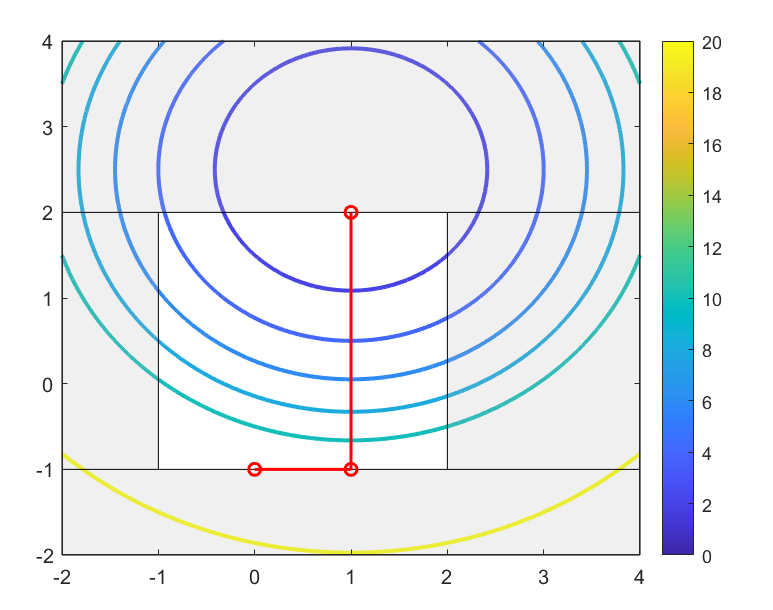
\includegraphics[scale=0.4]{figures/QP_AS_2_A.PNG}
%\caption{fig1}
}
\quad
\subfigure[$B(2,0)$]{
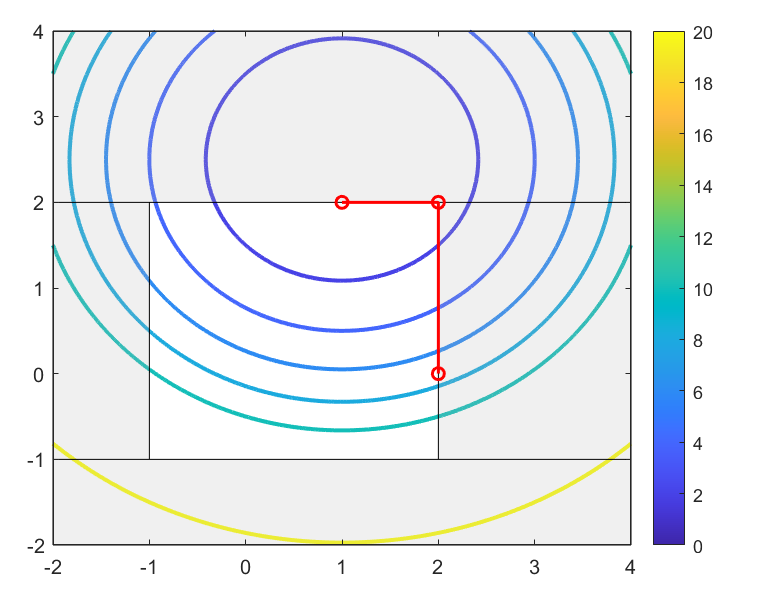
\includegraphics[scale=0.4]{figures/QP_AS_2_B.PNG}
}
\quad
\subfigure[$C(0,2)$]{
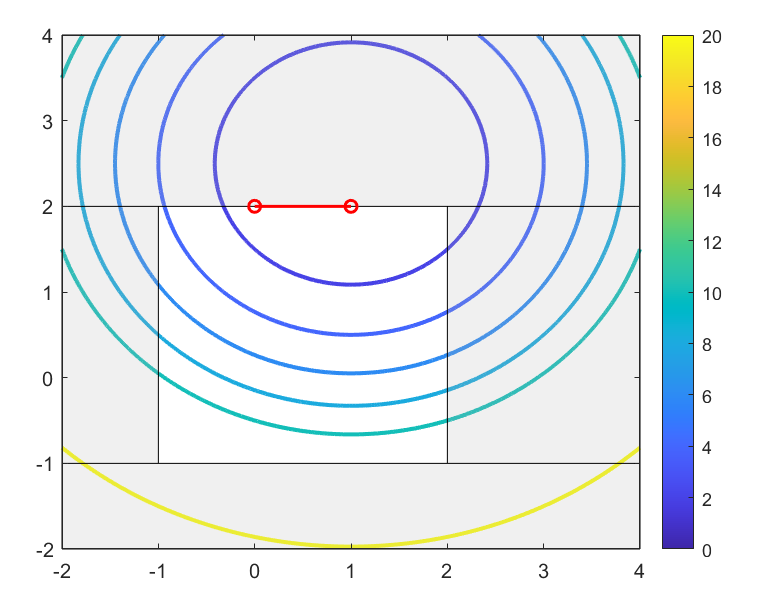
\includegraphics[scale=0.4]{figures/QP_AS_2_C.PNG}
}
\quad
\subfigure[$D(-1,0)$]{
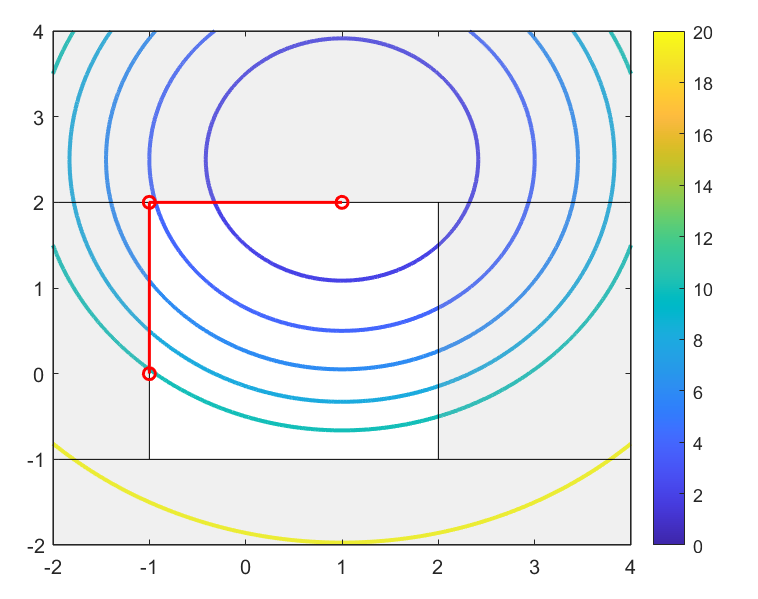
\includegraphics[scale=0.4]{figures/QP_AS_2_D.PNG}
}
\caption{ Iterative trajectory in contour of problem2}
\end{figure}

Also in the test of question 2, the four initial points all reached the minimum point under the constraint of inequality with a small number of iterations.
%%%%%%%%%%%%%%%%%%%%%%%%%%%%%%%%%%%%%%%%%%%%%%%%%%%%%%%%%%%%%%%%%%%%%%%%%%%%%%%%%%%%%%%%%%%%%%%%%%%%%%%%%%%%%%%%%%%%%%%%%%%%%%%%%%%%%%%%%%%%%%%%%%%%%%%%%%%%%%%%%%%%%%%%%%%%%%%%%%%%%%%%%%%%%%%%
\newpage
\subsection{\bfseries Comparison of algorithms}
\begin{shaded}
{Question: Compare the performance of your primal-dual interior-point algorithm, primal
active-set algorithm, and quadprog of Matlab (or equivalent QP library functions). Provide scripts that demonstrate how you compare the software and comment on the tests and the results.}
\end{shaded}
In order to better test the performance of the algorithm, a test problem that can randomly generate parameters and adjust the number and size of variables is designed.
\begin{align*}
&\min_{x} \quad \phi=\frac{1}{2} x^{\prime} H x+g^{\prime} x \qquad H\in \mathbb{R}^{n \times n} \quad g\in \mathbb{R}^{n \times 1} \tag{2.28}\label{con:op2.28}\\
& s.t. \quad A^{\prime}x=b \qquad \qquad \qquad A\in \mathbb{R}^{n \times m}\\
& \quad \quad  0\le x \le 10
\end{align*}
From the optimality conditions, it is  defined that
\begin{align*}
&x_{i}=\left\{\begin{array}{ll}
\text { random positive number } & i=1,2, \ldots, m \\
0 & i=m+1, m+2, \ldots, n
\end{array}\right \tag{2.29}\\
& z_{i}=\left\{\begin{array}{ll}
\text { random positive number } & i=m+1, m+2, \ldots, n \\
0 & i=1,2, \ldots, m
\end{array}\right \tag{2.30}\\
& y=\text{random vector}\\
& \nabla_{x} L\left(x,y,z\right)=Hx+g-Ay-z=0 \Leftrightarrow g=Ay+z-Hx\tag{2.31}\\
& \nabla_{y} L\left(x,y,z\right)=-\left(A^{\prime}x-b\right)=0 \Leftrightarrow b=A^{\prime}x\tag{2.32}\\
\end{align*}
Where the positive definite Hessian $H$ is designed by $H=P^{\prime}HP+Q, \quad P\in \mathbb{R}^{n \times n}, Q\in \mathbb{R}^{n \times n}$, The $P$ matrix is random positive matrix and $Q$ is an identity matrix.
In order to compare the performance of these two algorithms and quadprog, first the same initial feasible point solved by the method stated in active-set method(Here the "dual simplex method" in linprog is used) is used for three algorithms. And the iteration numbers and deviation expressed by $\left\|x^*-x_{result}\right\|_2$($x^*$ is the correct optimal solution and $x_{result}$ is the optimal solution obtained by the prim-dual interior point method) is showed to analyze the performance. Here the number of variables($n$) is adjusted from $10-200$ Please see the driver files in the appendix \ref{6.2.6}.
\begin{figure}[H]
\centering
\setlength{\abovecaptionskip}{-0.2cm} 
\setlength{\belowcaptionskip}{-0.5cm} 
\subfigure[Deviation]{
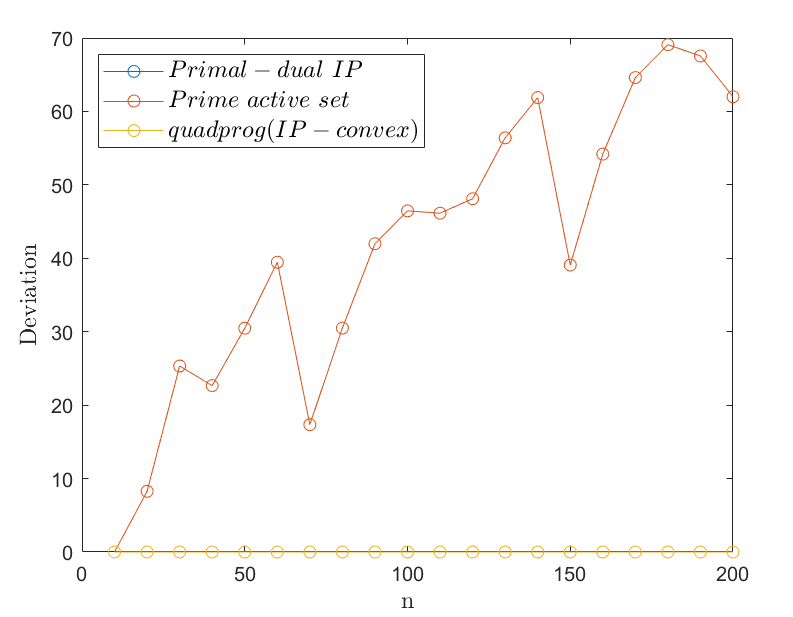
\includegraphics[scale=0.5]{figures/QP_ACCURACY.PNG}
%\caption{fig1}
}
\quad
\subfigure[Iteration numbers]{
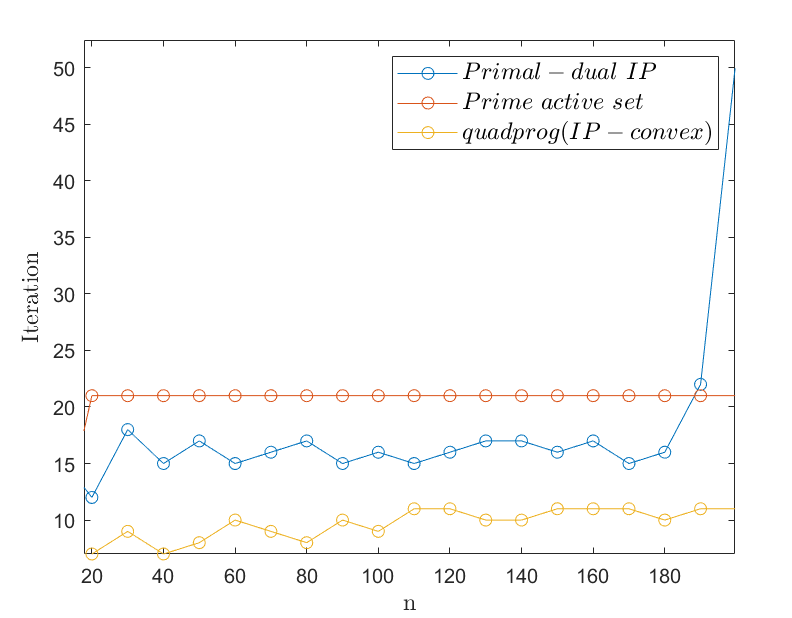
\includegraphics[scale=0.5]{figures/QP_ITERATION.PNG}
}
\caption{Performance of prime-dual interior-point algorithm, primal
active-set algorithm, and quadprog}
\end{figure}
First of all, for the deviation curve obtained by the three algorithms, it should be noted that the deviation curve obtained by the interior point method used by quadprog is exactly the same as the deviation curve of the prime-dual interior point method implemented by ourselves, so only two curves are displayed. It can be seen that as the number of variables increases, the deviation of the active set method gradually becomes larger, and the deviation of the obtained result from the correct value obtained by either the interior point method implemented or the interior point method using quadprog can be kept at a small value all the time, and does not increase with the increase of the number of variables.\\

Then for the curve of the number of iterations obtained by the three algorithms, it first can be seen that no matter how the number of variables increases, the interior point method of quadprog has been kept at a small number of iterations. It can be seen that when the number of variables is less than 180($n<180$), Although the number of iterations of the interior point method implemented is smaller than that of the active set method, when the number of variables is greater than 180($n>180$) , the number of iterations of the interior point method suddenly jumps more than the number of iterations of the active set method, and the iteration of the active set method has been stable at about 20 times, and does not change with the increase of the number of variables. It can be inferred that the reason for this difference may be 1. The stopping criteria set by the interior point method implemented and the quadprog interior point method are different 2. The starting point of the interior point method implemented and the interior point method of quadprog is the starting point calculated by the active set method, which may affect the number of iterations.

%%%%%%%%%%%%%%%%%%%%%%%%%%%%%%%%%%%%%%%%%%%%%%%%%%%%%%%%%%%%%%%%%%%%%%%%%%%%%%%%%%%%%%%%%%%%%%%%%%%%%%%%%%%%%%%%%%%%%%%%%%%%%%%%%%%%%%%%%%%%%%%%%%%%%%%%%%%%%%%%%%%%%%%%%%%%%%%%%%%%%%%%%%%%%%%%%%%%%%%%%%%%%%%%%%%%%%%%%%%%%%%%%%%%%%%%%%%%%%%%%%%%%%%%%%%%%%%%%%%%%%%%
 \subsection{\bfseries Markowitz’ portfolio optimization problem as QP}
\begin{shaded}
{Question: Demonstrate that Markowitz’ portfolio optimization problem can be expressed as
a QP in the form and test the primal-dual interior-point QP algorithm, the
primal active-set QP algorithm, and the library QP algorithm e.g. quadprog}
\end{shaded}
Consider a financial market with 5 securities.\\[0.3cm]
\begin{tabular}{c|ccccc|c}
\hline Security & \multicolumn{5}{|c|} { Covariance } &  Return\\
\hline 1 & 2.30 & 0.93 & 0.62 & 0.74 & -0.23 & 15.10 \\
2 & 0.93 & 1.40 & 0.22 & 0.56 & 0.26 & 12.50 \\
3 & 0.62 & 0.22 & 1.80 & 0.78 & -0.27 & 14.70 \\
4 & 0.74 & 0.56 & 0.78 & 3.40 & -0.56 & 9.02 \\
5 & -0.23 & 0.26 & -0.27 & -0.56 & 2.60 & 17.68 \\
\hline
\end{tabular}\\[0.3cm]
The quadratic programming form of Markowitz’ portfolio optimization problem
\begin{align*}
&\min_{x \in \mathcal{R}^n} \quad \phi=\frac{1}{2}x^{\prime}Hx \tag{2.33}\\
& s.t. \quad \mu^{\prime}x= R\\
& \quad \quad \sum_{i=1}^{n}x_i=1\\
& \quad \quad \ x \ge 0
\end{align*}
Then a portfolio with return, $R = 10.0$ is computed, to obtain minimal risk and the optimal
portfolio, by the primal-dual interior-point QP algorithm, the
primal active-set QP algorithm, and the "quadprog"(The interior-point-convex is used here). Please see the driver files in appendix \ref{6.2.7}. The result and the iteration numbers are showed\\
The primal-dual interior-point QP algorithm
\begin{align*}
&    x=(0,0.2816,0,0.7184,0)^{\prime}\\
&Return: \quad E\{ R\}=10\\
&Risk(Variance):\quad V\{ R\}=x^{\prime}Hx=2.0923\\
&Iteration=6
\end{align*}
The
primal active-set QP algorithm
\begin{align*}
&    x=(0,0.2816,0,0.7184,0)^{\prime}\\
&Return: \quad E\{ R\}=10\\
&Risk(Variance):\quad V\{ R\}=x^{\prime}Hx=2.0923\\
&Iteration=4
\end{align*}
The "quadprog" with "interior-point-convex"
\begin{align*}
&    x=(0,0.2816,0,0.7184,0)^{\prime}\\
&Return: \quad E\{ R\}=10\\
&Risk(Variance):\quad V\{ R\}=x^{\prime}Hx=2.0923\\
&Iteration=5
\end{align*}
\newpage
\section{ \bfseries Markowitz Portfolio Optimization}
This exercise illustrates use of quadratic programming in a financial application. By diversifying an investment into several securities it may be possible to reduce risk without reducing return. Identification and construction of such portfolios is called hedging. The Markowitz Portofolio Optimization problem is very simple hedging problem for
which Markowitz was awarded the Nobel Price in 1990.\\[0.3cm]
Consider a financial market with 5 securities.\\[0.3cm]
\begin{tabular}{c|ccccc|c}
\hline Security & \multicolumn{5}{|c|} { Covariance } &  Return\\
\hline 1 & 2.30 & 0.93 & 0.62 & 0.74 & -0.23 & 15.10 \\
2 & 0.93 & 1.40 & 0.22 & 0.56 & 0.26 & 12.50 \\
3 & 0.62 & 0.22 & 1.80 & 0.78 & -0.27 & 14.70 \\
4 & 0.74 & 0.56 & 0.78 & 3.40 & -0.56 & 9.02 \\
5 & -0.23 & 0.26 & -0.27 & -0.56 & 2.60 & 17.68 \\
\hline
\end{tabular}

%%%%%%%%%%%%%%%%%%%%%%%%%%%%%%%%%%%%%%%%%%
%%%%%%%%%%%%%%%%%%%%%%%%%%%%%%%%%%%%%%%%%%%%%%%%%%%%%%%%%%%%%%%%%%%%%%%%%%%%%%%%%%%%%
%%%%%%%%%%%%%%%%%%%%%%%%%%%%%%%%%%%%%%%%%%%
%%%%%%%%%%%%%%%%%%%%%%%%%%%%%%%%%%%%%%%%%%
%%%%%%%%%%%%%%%%%%%%%%%%%%%%%%%%%%%%%%%%%%%
\subsection{\bfseries Original problem}
%%%%%%%%%%%%%%%%%%%%%%%%%%%%%%%%%%%%%%%%%%
%%%%%%%%%%%%%%%%%%%%%%%%%%%%%%%%%%%%%%%%%%%%%%%%%%%%%%%%%%%%%%%%%%%%%%%%%%%%%%%%%%%%%
%%%%%%%%%%%%%%%%%%%%%%%%%%%%%%%%%%%%%%%%%%%
%%%%%%%%%%%%%%%%%%%%%%%%%%%%%%%%%%%%%%%%%%
%%%%%%%%%%%%%%%%%%%%%%%%%%%%%%%%%%%%%%%%%%%
\subsubsection{\bfseries Formulation}
\begin{shaded}
{ Question: For a given return, $R$, formulate Markowitz’ Portfolio optimization problem as a quadratic program.}
\end{shaded}
\begin{align*}
&\min_{x \in \mathcal{R}^n} \quad \phi=\frac{1}{2}x^{\prime}Hx \tag{3}\\
& s.t. \quad \mu^{\prime}x\ge R\\
& \quad \quad \sum_{i=1}^{n}x_i=1\\
& \quad \quad \ x \ge 0
\end{align*}
Required return is $R$, expected return and variance of the portfolio\\
\begin{align*}
\bar{R}=E\{ R\}&=E\{ r^{\prime}x\}=\mu^{\prime}x \tag{3.1}\\
 V\{ R\}&=E\{(R-\bar{R})^2 \}=E{x^{\prime}(r-\mu)(r-\mu)^{\prime}x}=x^{\prime}Hx \tag{3.2}\\
\end{align*}

%%%%%%%%%%%%%%%%%%%%%%%%%%%%%%%%%%%%%%%%%%
%%%%%%%%%%%%%%%%%%%%%%%%%%%%%%%%%%%%%%%%%%%%%%%%%%%%%%%%%%%%%%%%%%%%%%%%%%%%%%%%%%%%%
%%%%%%%%%%%%%%%%%%%%%%%%%%%%%%%%%%%%%%%%%%%
%%%%%%%%%%%%%%%%%%%%%%%%%%%%%%%%%%%%%%%%%%
%%%%%%%%%%%%%%%%%%%%%%%%%%%%%%%%%%%%%%%%%%%
\subsubsection{\bfseries Minimal and maximal return}
\begin{shaded}
{ Question: What is the minimal and maximal possible return in this financial market?}
\end{shaded}
If the variance of the protfolio is not considered, the security 4 can only be invested to obtain the minimal return 9.02, or only invest in security 5 to obtain maximal return 17.68.
%%%%%%%%%%%%%%%%%%%%%%%%%%%%%%%%%%%%%%%%%%
%%%%%%%%%%%%%%%%%%%%%%%%%%%%%%%%%%%%%%%%%%%%%%%%%%%%%%%%%%%%%%%%%%%%%%%%%%%%%%%%%%%%%
%%%%%%%%%%%%%%%%%%%%%%%%%%%%%%%%%%%%%%%%%%%
%%%%%%%%%%%%%%%%%%%%%%%%%%%%%%%%%%%%%%%%%%
%%%%%%%%%%%%%%%%%%%%%%%%%%%%%%%%%%%%%%%%%%%
\subsubsection{\bfseries Optimal
portfolio}
\begin{shaded}
{ Question: Compute a portfolio with return, $R = 10.0$, and minimal risk. What is the optimal portfolio and what is the risk (variance)?}
\end{shaded}
To achieve a return of exactly 10 then the constraint $\mu^{\prime}x\ge R$ have to be changed to an equlity constraint $\mu^{\prime}x= R$. The Matlab function $quadprog$ is used to solve the constructed problem. Please see the driver files in appendix \ref{6.3.1}. The calculated optimal portfolio is 
\begin{align*}
&    x=(0,0.2816,0,0.7184,0)^{\prime}\\
&Return: \quad E\{ R\}=10\\
&Risk(Variance):\quad V\{ R\}=x^{\prime}Hx=2.0923
\end{align*}

However, the highest possible return with the minimum variance is generally desired. The original constraint is maintained  $\mu^{\prime}x\ge R$ to get the highest possible return and greater than 10. Please see the driver files in appendix \ref{6.3.2}. The optimal portfolio is 
 \begin{align*}
&    x=(0.0883,0.2509,0.2824,0.1038,0.2748)^{\prime}\\
&Return: \quad E\{ R\}=14.4129\\
&Risk(Variance):\quad V\{ R\}=x^{\prime}Hx=0.6249
\end{align*}
%%%%%%%%%%%%%%%%%%%%%%%%%%%%%%%%%%%%%%%%%%
%%%%%%%%%%%%%%%%%%%%%%%%%%%%%%%%%%%%%%%%%%%%%%%%%%%%%%%%%%%%%%%%%%%%%%%%%%%%%%%%%%%%%
%%%%%%%%%%%%%%%%%%%%%%%%%%%%%%%%%%%%%%%%%%%
%%%%%%%%%%%%%%%%%%%%%%%%%%%%%%%%%%%%%%%%%%
%%%%%%%%%%%%%%%%%%%%%%%%%%%%%%%%%%%%%%%%%%%
\subsubsection{\bfseries Efficient frontier}
\begin{shaded}
{ Question:  Compute the efficient frontier, i.e. the risk as function of the return. Plot the efficient frontier as well as the optimal portfolio as function of return.}
\end{shaded}
\begin{figure}[H]
\centering
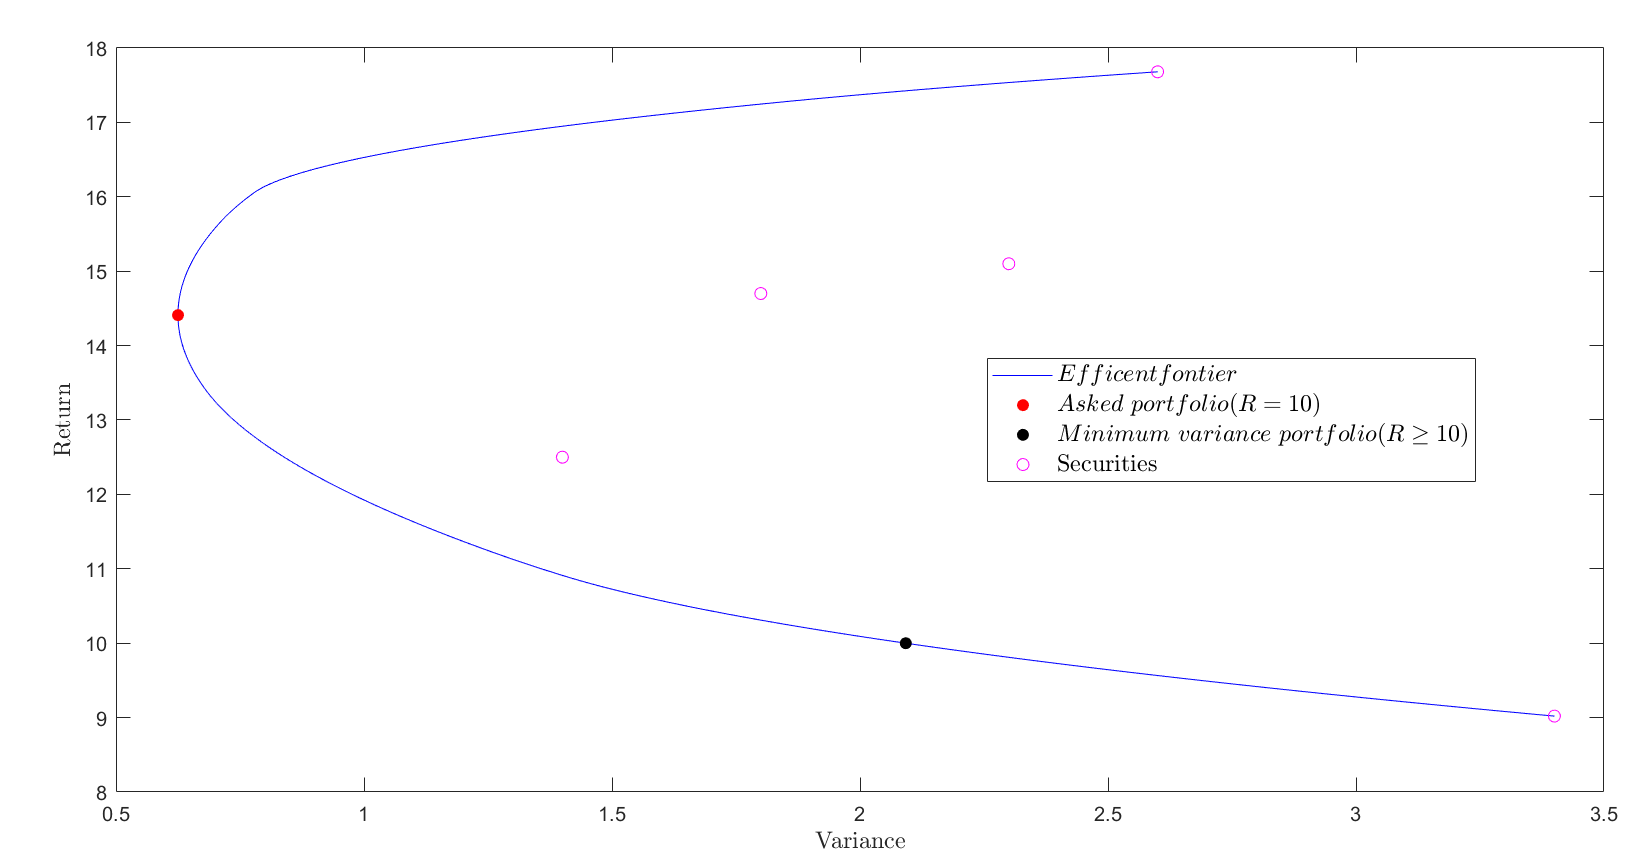
\includegraphics[scale=0.5]{figures/eff_fro1.PNG}
\caption{Efficient frontier of the portfolio}
\label{fig:labe3.1.4}
\end{figure}
Where the black filled dot is the asked portfolio($R=10$), and the red filled dot is the minimum variance and the return is also satisfied the asked portfolio. The pink unfilled dot is the securities. Please see the driver files in appendix \ref{6.3.3}.

%%%%%%%%%%%%%%%%%%%%%%%%%%%%%%%%%%%%%%%%%%
%%%%%%%%%%%%%%%%%%%%%%%%%%%%%%%%%%%%%%%%%%%%%%%%%%%%%%%%%%%%%%%%%%%%%%%%%%%%%%%%%%%%%
%%%%%%%%%%%%%%%%%%%%%%%%%%%%%%%%%%%%%%%%%%%
%%%%%%%%%%%%%%%%%%%%%%%%%%%%%%%%%%%%%%%%%%
%%%%%%%%%%%%%%%%%%%%%%%%%%%%%%%%%%%%%%%%%%%
\newpage
\subsection{\bfseries Problem with an added risk free security}
%%%%%%%%%%%%%%%%%%%%%%%%%%%%%%%%%%%%%%%%%%
%%%%%%%%%%%%%%%%%%%%%%%%%%%%%%%%%%%%%%%%%%%%%%%%%%%%%%%%%%%%%%%%%%%%%%%%%%%%%%%%%%%%%
%%%%%%%%%%%%%%%%%%%%%%%%%%%%%%%%%%%%%%%%%%%
%%%%%%%%%%%%%%%%%%%%%%%%%%%%%%%%%%%%%%%%%%
%%%%%%%%%%%%%%%%%%%%%%%%%%%%%%%%%%%%%%%%%%%
\subsubsection{\bfseries New covariance matrix and return vector}
\begin{shaded}
{ Question: What is the new covariance matrix and return vector}
\end{shaded}
The new covariance matrix and return vector is
$$H=\begin{bmatrix}
2.30 & 0.93 & 0.62 & 0.74 & -0.23 & 0 \\
0.93 & 1.40 & 0.22 & 0.56 & 0.26 & 0 \\
0.62 & 0.22 & 1.80 & 0.78 & -0.27 & 0 \\
0.74 & 0.56 & 0.78 & 3.40 & -0.56 & 0 \\
-0.23 & 0.26 & -0.27 & -0.56 & 2.60 & 0 \\
0 & 0 & 0 & 0 & 0 &0
\end{bmatrix}\quad \mu=\begin{bmatrix}
15.10\\
12.50\\
14.70\\
9.02\\
17.68\\
2.0
\end{bmatrix}$$
%%%%%%%%%%%%%%%%%%%%%%%%%%%%%%%%%%%%%%%%%%
%%%%%%%%%%%%%%%%%%%%%%%%%%%%%%%%%%%%%%%%%%%%%%%%%%%%%%%%%%%%%%%%%%%%%%%%%%%%%%%%%%%%%
%%%%%%%%%%%%%%%%%%%%%%%%%%%%%%%%%%%%%%%%%%%
%%%%%%%%%%%%%%%%%%%%%%%%%%%%%%%%%%%%%%%%%%
%%%%%%%%%%%%%%%%%%%%%%%%%%%%%%%%%%%%%%%%%%%
\subsubsection{\bfseries Efficient frontier with optimal
portfolio when $R=10$}
\begin{shaded}
{ Question: Compute the efficient frontier, plot it as well as the (return,risk) coordinates of all the securities. Comment on the effect of a risk free security. Plot the optimal portfolio as function of return.}
\end{shaded}
\begin{figure}[H]
\centering
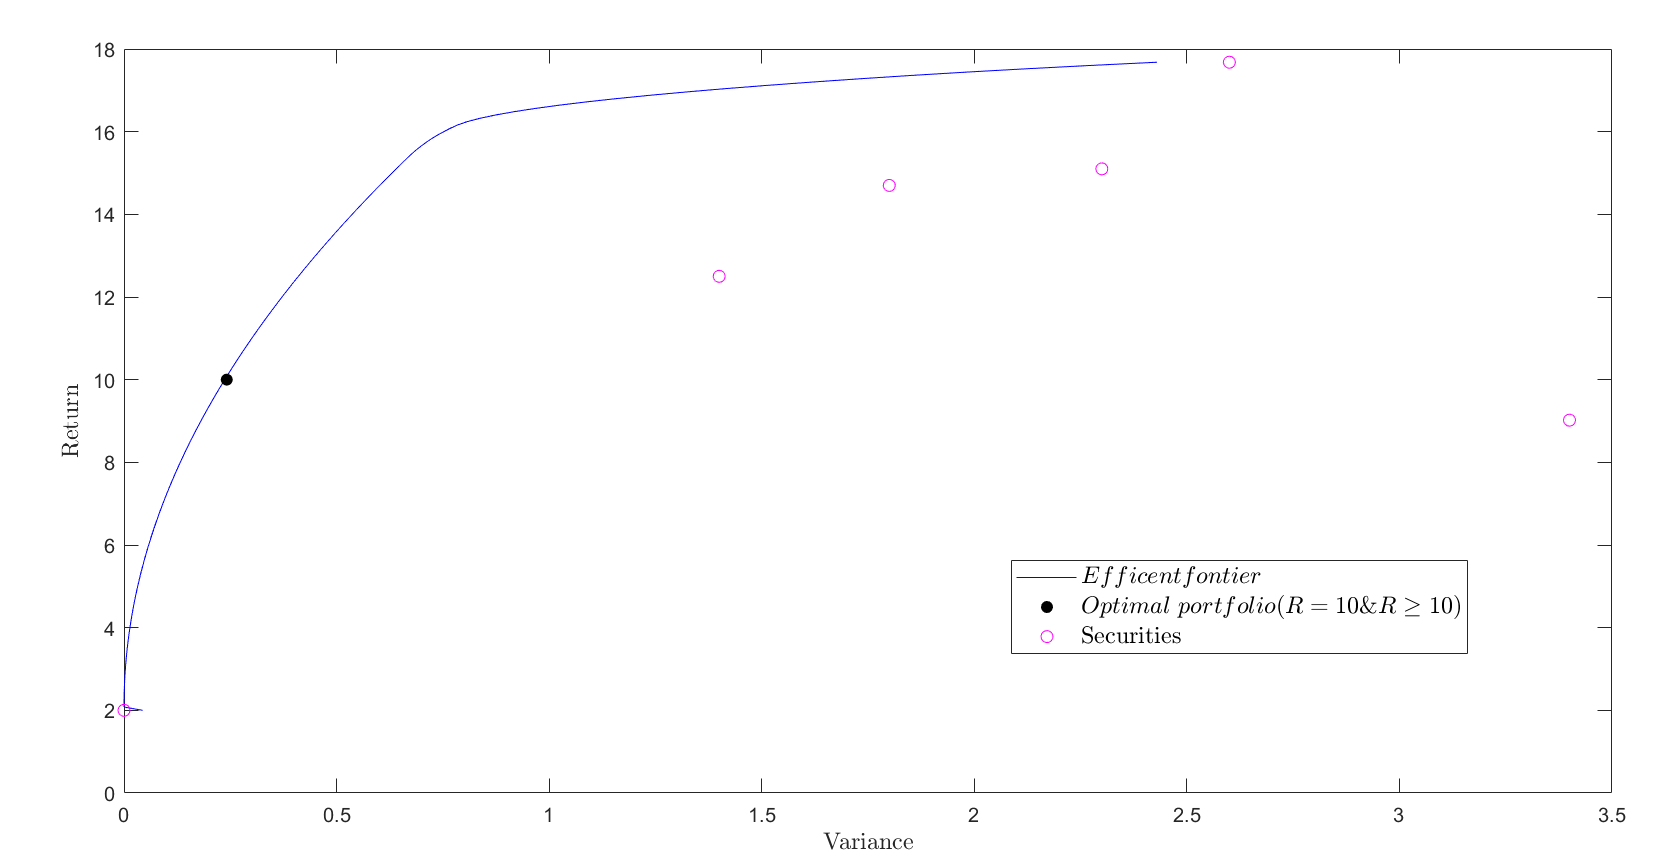
\includegraphics[scale=0.5]{figures/eff_fro2.PNG}
\caption{Efficient frontier with optimal
portfolio when $R=10$}
\label{fig:labe3.2.2}
\end{figure}
It can be seen that regardless of whether $R \ge 10$ or $R=10$, the same solution will be obtained(the black filled point). The reason can be found in the efficient frontier. After adding a risk free security, it is found that the efficient frontier increases monotonously. That is to say, when a portfolio with a higher return than or equal to a specific value and require minimum variance is desired, the variance corresponding to the higher return value is smaller than the variance corresponding to this asked return value cannot be found. Please see the driver files in appendix \ref{6.3.4}.


%%%%%%%%%%%%%%%%%%%%%%%%%%%%%%%%%%%%%%%%%%
%%%%%%%%%%%%%%%%%%%%%%%%%%%%%%%%%%%%%%%%%%%%%%%%%%%%%%%%%%%%%%%%%%%%%%%%%%%%%%%%%%%%%
%%%%%%%%%%%%%%%%%%%%%%%%%%%%%%%%%%%%%%%%%%%
%%%%%%%%%%%%%%%%%%%%%%%%%%%%%%%%%%%%%%%%%%
%%%%%%%%%%%%%%%%%%%%%%%%%%%%%%%%%%%%%%%%%%%
\subsubsection{\bfseries Optimal portfolio when $R=15$}
\begin{shaded}
{ Question: What is the minimal risk and optimal portfolio giving a return of $R = 15.00$. Plot
this point in your optimal portfolio as function of return as well as on the efficient
frontier diagram.}
\end{shaded}
when $R=15.00$ or $R\ge 15.00$
\begin{align*}
&    x=(0.1655,0.1365,0.3115,0.0266,0.3352,0.0247)^{\prime}\\
&Return: \quad E\{ R\}=15.00\\
&Risk(Variance):\quad V\{ R\}=x^{\prime}Hx=0.6383
\end{align*}
\begin{figure}[H]
\centering
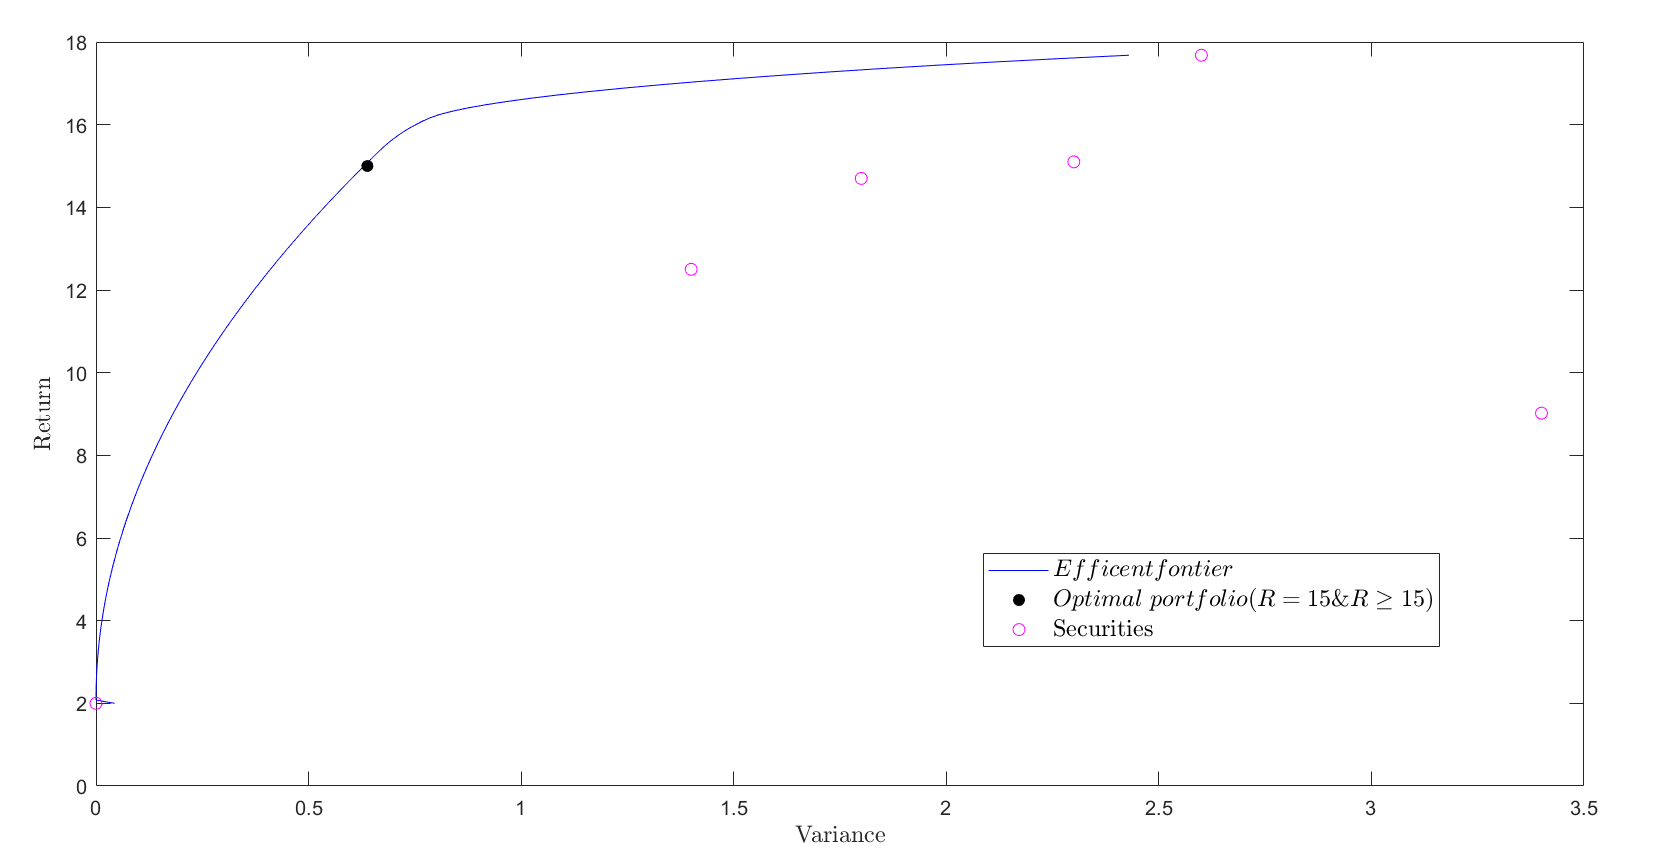
\includegraphics[scale=0.5]{figures/eff_fro3.PNG}
\caption{Efficient frontier with optimal
portfolio when $R=15$ }
\label{fig:labe3.2.2}
\end{figure}
Where the black filled dot is the optimal  portfolio when $R=10$ or $R=15$, and the pink unfilled dot is the securities.

\newpage
\section{ \bfseries Linear Program (LP)}
In this problem, a linear program in the form (assume that $A$ has full column rank) is considered.\\
\begin{align*}
&\min_{x} \quad \phi=g^{\prime} x \tag{4}\label{con:op4.1}\\
& s.t. \quad A^{\prime} x=b\\
& \quad \quad  l\le x \le u
\end{align*}
%%%%%%%%%%%%%%%%%%%%%%%%%%%%%%%%%%%%%%%%%%
%%%%%%%%%%%%%%%%%%%%%%%%%%%%%%%%%%%%%%%%%%%%%%%%%%%%%%%%%%%%%%%%%%%%%%%%%%%%%%%%%%%%%
%%%%%%%%%%%%%%%%%%%%%%%%%%%%%%%%%%%%%%%%%%%
%%%%%%%%%%%%%%%%%%%%%%%%%%%%%%%%%%%%%%%%%%
%%%%%%%%%%%%%%%%%%%%%%%%%%%%%%%%%%%%%%%%%%%
\subsection{\bfseries Lagrangian function}
\begin{shaded}
{ Question: What is the Lagrangian function for this problem?}
\end{shaded}
The linear program problem (\ref{con:op4.1}) are usually stated and analyzed in the standard form, the inequlity constraints can be converted to equalities by introducing a vector of slack variables $z$ and writing

\begin{align*}
&\min_{x} \quad \phi=g^{\prime} x \tag{4.1}\\
& s.t. \quad A^{\prime} x=b\\
& \quad \quad  c(x)=\begin{bmatrix}
x-l \\ u-x\end{bmatrix}=\left[I\quad -I\right]^{\prime}x+\begin{bmatrix}
-l \\ u\end{bmatrix}\ge 0\Leftrightarrow C^{\prime}x \ge d\Leftrightarrow C^{\prime}x-z=d(z\ge 0)
\end{align*}\\[0.3cm]

The equality constraints in linear programming is always treated as $x \ge 0$ and the lagrange multipliers $\lambda$ and $s$ are introduced.The Lagrangian function is\\
$$L(x,\lambda,s)=g^{\prime}x-\lambda^{\prime}\left(A^{\prime}x-b\right)-s^{\prime}x\eqno{(4.2)}$$

%%%%%%%%%%%%%%%%%%%%%%%%%%%%%%%%%%%%%%%%%%
%%%%%%%%%%%%%%%%%%%%%%%%%%%%%%%%%%%%%%%%%%%
%%%%%%%%%%%%%%%%%%%%%%%%%%%%%%%%%%%%%%%%%%
%%%%%%%%%%%%%%%%%%%%%%%%%%%%%%%%%%%%%%%%%%%
%%%%%%%%%%%%%%%%%%%%%%%%%%%%%%%%%%%%%%%%%%
%%%%%%%%%%%%%%%%%%%%%%%%%%%%%%%%%%%%%%%%%%%
\newpage
\subsection{\bfseries Optimality conditions}
\begin{shaded}
{Question: Write the nesessary and sufficient optimality conditions for this problem.}
\end{shaded}
\begin{align*}
& \nabla_{x} L\left(x,\mu,\lambda\right)=g-A\lambda-s=0\tag{4.3}\\
& \nabla_{\lambda} L\left(x,\mu,\lambda\right)=-\left(A^{\prime}x-b\right)=0\tag{4.4}\\
& \nabla_{s} L\left(x,\mu,\lambda\right)=x \ge 0\tag{4.5}\\
& s \ge 0\tag{4.6}\\
& x_is_i=0 \quad i=1,2,...,n\tag{4.7}
\end{align*}

%%%%%%%%%%%%%%%%%%%%%%%%%%%%%%%%%%%%%%%%%%
%%%%%%%%%%%%%%%%%%%%%%%%%%%%%%%%%%%%%%%%%%%
%%%%%%%%%%%%%%%%%%%%%%%%%%%%%%%%%%%%%%%%%%
%%%%%%%%%%%%%%%%%%%%%%%%%%%%%%%%%%%%%%%%%%%
%%%%%%%%%%%%%%%%%%%%%%%%%%%%%%%%%%%%%%%%%%
%%%%%%%%%%%%%%%%%%%%%%%%%%%%%%%%%%%%%%%%%%%
\subsection{\bfseries Primal-dual interior-point algorithm}
\begin{shaded}
{Question: Write pseudo-code for a primal-dual interior-point algorithm for solution of this
problem. Explain each major step in your algorithm.}
\end{shaded}

{\setmainfont{Times New Roman}\bfseries Pseudo-code}
\begin{algorithm}[!h]
	\caption{Primal-Dual Predictor-Corrector Interior-Point Algorithm}
	\begin{algorithmic}[1]
	    \STATE Given an input $H$, $g$, $A$, $b$, and compute the starting point $x_0$, $\lambda_0$, $s_0$ with ($x_0$,$s_0$)>0\\
        \WHILE {(not converged)}\\
		\STATE Compute the affine step direction $\Delta x^{aff}$, $\Delta \lambda^{aff}$ and $\Delta s^{aff}$\\
		\STATE Compute the affine step size\  $\alpha_{aff}^{pri}$\ and\ $\alpha_{aff}^{dual}$\\
		\STATE Compute the affine duality gap $\mu_{aff} $\\
		\STATE Compute centering parameter $\sigma=\left(\mu_{aff}/\mu\right)^3$\\
		\STATE Compute affine-centering-correction direction$(\Delta x,\Delta \lambda,\Delta s)$\\
		\STATE Compute the step size $\alpha * \eta$ and update the iteration of $x^{k+1}=x^k+\alpha_k^{pri}\Delta x$, $(\lambda^{k+1},s^{k+1})=(\lambda^k,s^k)+\alpha_k^{dual}(\Delta \lambda,\Delta s)$ and $s$ to take the actual step\\
		\STATE Check convergence conditions and stop if it converged\\
		\ENDWHILE
    \end{algorithmic}
\end{algorithm}
\newpage
In the first step, a set of feasible starting point needs to be computed. A heuristic for starting point on p.410 in Nocedal \& Wright is introduced\\[0.3cm]
The problems is solved 
\begin{align*}
&\min _{x} \quad\frac{1}{2} x^{\prime} x  \qquad s.t. \quad A^{\prime}x=b \tag{4.8}\\
&\min _{(\lambda, s)} \quad\frac{1}{2} s^{\prime} s \qquad  s.t. \quad  A \lambda+s=g\tag{4.9}
\end{align*}
$\tilde{x}$, $\tilde{\lambda}$ and $\tilde{s}$ can be written as
$$\tilde{x}=A\left(A^{\prime} A\right)^{-1} b \quad \tilde{\lambda}=\left(A^{\prime} A\right)^{-1} A^{\prime} g, \quad \tilde{s}=g-A \tilde{\lambda}\eqno{(4.10)}$$
Because $\tilde{x}$ and $\tilde{s}$ should be greater than $0$
$$\delta_{x}=\max \left(-(3 / 2) \min _{i} \tilde{x}_{i}, 0\right), \delta_{s}=\max \left(-(3 / 2) \min _{i} \tilde{s}_{i}, 0\right)\eqno{(4.11)}$$
$$\hat{x}=\tilde{x}+\delta_{x} e \quad \hat{s}=\tilde{s}+\delta_{s} e \quad e=(1, \ldots, 1)^{T}$$
To ensure that the components $x^0$ and $s^0$ is not to0 close to zero or too dissimilar, two more scalars are added
$$\hat{\delta}_{x}=\frac{1}{2} \frac{\hat{x}^{T} \hat{s}}{e^{T} \hat{s}}, \quad \hat{\delta}_{s}=\frac{1}{2} \frac{\hat{x}^{T} \hat{s}}{e^{T} \hat{x}}\eqno{(4.12)}$$
$$x^{0}=\hat{x}+\hat{\delta}_{x} e, \quad \lambda^{0}=\tilde{\lambda}, \quad s^{0}=\hat{s}+\hat{\delta}_{s} e$$
The spirit of the Primal-dual interior-point algorithm for linear programming is similar to the ones for quadratic Programming, and the specific calculation process is as follows.\\[0.3cm]
First the optimal conditions
$$F(x, \lambda, s)=\left[\begin{array}{c}
A \lambda+s-g \\
A^{\prime} x-b \\
X S e
\end{array}\right]=0\eqno{(4.13)}$$
Where
$$X=\operatorname{diag}\left(x_{1}, \ldots, x_{n}\right),\quad S=\operatorname{diag}\left(s_{1}, \ldots, s_{n}\right)$$
The affine step direction is solved by
$$\left[\begin{array}{lll}
0 & A & I \\
A^{\prime} & 0 & 0 \\
S & 0 & X
\end{array}\right]\left[\begin{array}{l}
\Delta x^{\mathrm{aff}} \\
\Delta \lambda^{\mathrm{aff}} \\
\Delta s^{\mathrm{aff}}
\end{array}\right]=-\left[\begin{array}{c}
A \lambda+s-c \\
A^{\prime} x-b \\
X S e
\end{array}\right]=\left[\begin{array}{c}
-r_{c} \\
-r_{b} \\
-X S e
\end{array}\right]\eqno{(4.14)}$$
Then the affine step size can be calculated
$$\alpha_{\mathrm{aff}}^{\mathrm{pri}}=\min \left(1, \min _{i: \Delta x_{i}^{\mathrm{aff}}<0}-\frac{x_{i}}{\Delta x_{i}^{\mathrm{aff}}}\right), \quad \alpha_{\mathrm{aff}}^{\mathrm{dual}}=\min \left(1, \min _{i: \Delta s_{i}^{\mathrm{aff}}<0}-\frac{s_{i}}{\Delta s_{i}^{\mathrm{aff}}}\right)\eqno{(4.15)}$$
The Duality gap $\mu_{aff}$ is defined for affine step
$$\mu_{\mathrm{aff}}=\left(x+\alpha_{\mathrm{aff}}^{\mathrm{pri}} \delta x^{\mathrm{aff}}\right)^{T}\left(s+\alpha_{\mathrm{aff}}^{\mathrm{dual}} \delta s^{\mathrm{aff}}\right) / n\eqno{(4.16)}$$
The centering parameter
$$\sigma=\left(\frac{\mu_{\mathrm{aff}}}{\mu}\right)^{3}\eqno{(4.17)}$$
Affine-centering-correction direction is computed
$$\left[\begin{array}{ccc}
0 & A & I \\
A^{\prime} & 0 & 0 \\
S & 0 & X
\end{array}\right]\left[\begin{array}{c}
\Delta x \\
\Delta \lambda\\
\Delta s
\end{array}\right]=\left[\begin{array}{c}
-r_{c} \\
-r_{b} \\
-X S e+-\Delta X^{\mathrm{aff}} \Delta S^{\mathrm{aff}} e+\mu \sigma e
\end{array}\right]\eqno{(4.18)}$$
With the given direction, the step length can be found.\\[0.3cm]
The quantities are defined as
$$\alpha_{k, \max }^{\mathrm{pri}} \stackrel{\text { def }}{=} \min _{i: \Delta x_{i}^{k}<0}-\frac{x_{i}^{k}}{\Delta x_{i}^{k}}, \quad \alpha_{k, \max }^{\mathrm{dual}} \stackrel{\text { def }}{=} \min _{i: \Delta s_{i}^{k}<0}-\frac{s_{i}^{k}}{\Delta s_{i}^{k}}\eqno{(4.19)}$$
Then the step length 
$$\alpha_{k}^{\mathrm{pri}}=\min \left(1, \eta \alpha_{k, \max }^{\mathrm{pri}}\right), \quad \alpha_{k}^{\mathrm{dual}}=\min \left(1, \eta \alpha_{k, \max }^{\mathrm{dual}}\right)\eqno{(4.20)}$$
Finally the $x^{k+1}$, $\lambda^{k+1}$ and $s^{k+1}$ update and convergence conditions is checked and stop if it converged.



%%%%%%%%%%%%%%%%%%%%%%%%%%%%%%%%%%%%%%%%%%
%%%%%%%%%%%%%%%%%%%%%%%%%%%%%%%%%%%%%%%%%%%
%%%%%%%%%%%%%%%%%%%%%%%%%%%%%%%%%%%%%%%%%%
%%%%%%%%%%%%%%%%%%%%%%%%%%%%%%%%%%%%%%%%%%%
%%%%%%%%%%%%%%%%%%%%%%%%%%%%%%%%%%%%%%%%%%
%%%%%%%%%%%%%%%%%%%%%%%%%%%%%%%%%%%%%%%%%%%
\newpage
\subsection{\bfseries Implementation of primal-dual interior-point algorithm}
\begin{shaded}
{Question: Implement the primal-dual interior-point algorithm and test it. You must provide commented code as well as driver files to test your code, documentation that it works, and performance statistics.}
\end{shaded}
The matlab code is showed
{\setmainfont{Courier New Bold} \scriptsize            
\begin{lstlisting}
function [x,output]=ipLP(g,A,b)
% ipLP   Primal-dual interior-point algorithm
%
%          min  g'*x
%           x
%          s.t. A x  = b      
%               x >= 0      
%         rc = g − A*lambda − S = 0 
%         rb = Ax − b = 0 
%         XSe=0
%         rA = Ax + b = 0 (Lagrange multiplier y)
%         rC = Cx + s + d = 0 (Lagrange multiplier z)
%         s ≥ 0 (Slack variables )
%         sz = 0
% Syntax: [x,output]=ipLP(g,A,b)
%         output.fval: minimum value
%         output.lam : final lambda
%         output.s : final s
%         output.z: final z
%         output.Xarray: Iteration trajectory    
iteration_max=30;

epsilon=1.0e-6;
eta=0.99;
stop_flag=0;
nx=size(g,1);%x
nc=size(b,1);%c
%starting point
e=ones(nx,1);
x_hat=A'*inv(A*A')*b;
lam_hat=inv(A*A')*A*g;
s_hat=g-A'*lam_hat;

delta_x=max(-(3/2)*min(x_hat),0);
delta_s=max(-(3/2)*min(s_hat),0);

x_hat=x_hat+delta_x*e;
s_hat=s_hat+delta_s*e;

delta_x_hat=0.5*(x_hat'*s_hat)/(e'*s_hat);
delta_s_hat=0.5*(x_hat'*s_hat)/(e'*x_hat);

x0=x_hat+delta_x_hat*e;
lam0=lam_hat;
s0=s_hat+delta_s_hat*e;

Xarray=[];
Xarray=[Xarray x0];
%Predictor-Corrector algorithm
rc=A'*lam0+s0-g;
rb=A*x0-b;

x=x0;
lam=lam0;
s=s0;
iteration=0;
while(~stop_flag&iteration<=iteration_max)
    %solving the problem to obtain delta_x_aff,delta_lam_aff and delta_s_aff
    KKT_A=[zeros(nx,nx) A' eye(nx,nx);A zeros(nc,nc) zeros(nc,nx);diag(s) zeros(nx,nc) diag(x)];
    XSe=diag(x)*diag(s)*e;
    KKT_b=[-rc;-rb;-XSe];
    [L,D,p]=ldl(KKT_A, 'lower', 'vector');
    delta_aff=zeros(size(KKT_b,1),1);
    delta_aff(p)=L'\(D\(L\KKT_b(p)));
    delta_x_aff=delta_aff(1:nx);
    delta_lam_aff=delta_aff(nx+1:nx+nc);
    delta_s_aff=delta_aff(nx+nc+1:end);
    
    %calculate the alf_pri and alf_dual
    xi_deltax=-x./delta_x_aff;
    alf_pri=min([1;xi_deltax(delta_x_aff<0)]);
    si_deltas=-s./delta_s_aff;
    alf_dual=min([1;si_deltas(delta_s_aff<0)]);
    
    %calculate mu_aff and dual gap
    mu_aff=(x+alf_pri*delta_x_aff)'*(s+alf_dual*delta_s_aff)/nx;
    mu=(x'*s)/nx;
    %calculate centering parameter
    sigma=(mu_aff/mu)^3;
    %solving the problem to obtain delta_x_step, delta_lam_step and delta_s_step
    XSe_aff=-(diag(x)*diag(s)*e)-diag(delta_x_aff)*diag(delta_s_aff)*e+sigma*mu*e;
    KKT_b=[-rc;-rb;XSe_aff];
    delta_step=zeros(size(KKT_b,1),1);
    delta_step(p)=L'\(D\(L\KKT_b(p)));
    delta_x_step=delta_step(1:nx);
    delta_lam_step=delta_step(nx+1:nx+nc);
    delta_s_step=delta_step(nx+nc+1:end);
    
    %step length
    xk_deltaxk=-x./delta_x_step;
    alf_pri_k_max=min(xk_deltaxk(delta_x_step<0));
    alf_pri_k=min([1;eta*alf_pri_k_max]);
    
    sk_deltask=-s./delta_s_step;
    alf_dual_k_max=min(sk_deltask(delta_s_step<0));
    alf_dual_k=min([1;eta*alf_dual_k_max]);
    
    x=x+alf_pri_k*delta_x_step;
    lam=lam+alf_dual_k*delta_lam_step;
    s=s+alf_dual_k*delta_s_step;
    
    rc_norm=norm(rc,2);
    ra_norm=norm(rb,2);
    dual_gap=abs(x'*s/nx);
     %stop judge
    judge = [rc_norm;ra_norm;dual_gap];
    stop_flag = (length(judge(judge < epsilon)) == 3);
    %update rc and rb
    rc=(1-alf_dual_k)*rc;
    rb=(1-alf_pri_k)*rb;
    iteration=iteration+1;
    Xarray=[Xarray x];
end
fval=g'*x;
output.fval=fval;
output.lam=lam;
output.s=s;
output.iteration=iteration;
output.xarray=Xarray;
end
\end{lstlisting}}
In order to better test the performance of the algorithm, a test problem that can randomly generate parameters and adjust the number and size of variables is used.
\begin{align*}
&\min_{x} \quad \phi=g^{\prime} x \qquad g\in \mathbb{R}^{n \times 1} \tag{4.21}\label{con:op4.21}\\
& s.t. \quad A^{\prime}x=b \qquad \qquad \qquad A\in \mathbb{R}^{n \times m}\\
& \quad \quad  x\ge 0
\end{align*}

From the optimality conditions
\begin{align*}
&x_{i}=\left\{\begin{array}{ll}
\text { random positive number } & i=1,2, \ldots, m \\
0 & i=m+1, m+2, \ldots, n
\end{array}\right\tag{4.22}\\
& z_{i}=\left\{\begin{array}{ll}
\text { random positive number } & i=m+1, m+2, \ldots, n \\
0 & i=1,2, \ldots, m
\end{array}\right\tag{4.23}\\
& y=\text{random vector}\\
& \nabla_{x} L\left(x,y,z\right)=g-Ay-z=0 \Leftrightarrow g=Ay+z\tag{4.24}\\
& \nabla_{y} L\left(x,y,z\right)=-\left(A^{\prime}x-b\right)=0 \Leftrightarrow b=A^{\prime}x\tag{4.24}
\end{align*}
It is shown that the variable values($n$) range from 10 to 200, the curve of deviation expressed by $\left\|x^*-x_{result}\right\|_2$($x^*$ is the correct optimal solution and $x_{result}$ is the optimal solution obtained by the prim-dual interior point method), the curve of the objective function value corresponding to the $x_{*}$ and $x_{result}$ respectively, and the curve of the number of iterations. Please see the driver files in appendix.
\vspace{-0.5cm}
\begin{figure}[H]
\centering
\setlength{\abovecaptionskip}{-0.2cm} 
\setlength{\belowcaptionskip}{-0.5cm} 
\subfigure[Deviation]{
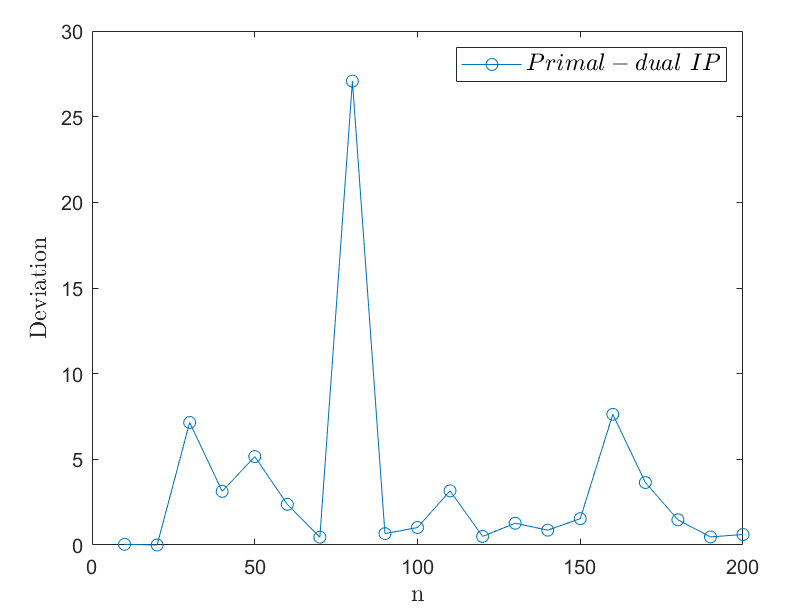
\includegraphics[scale=0.5]{figures/IP_IP_NORM.PNG}
%\caption{fig1}
}
\quad
\subfigure[Objective function value]{
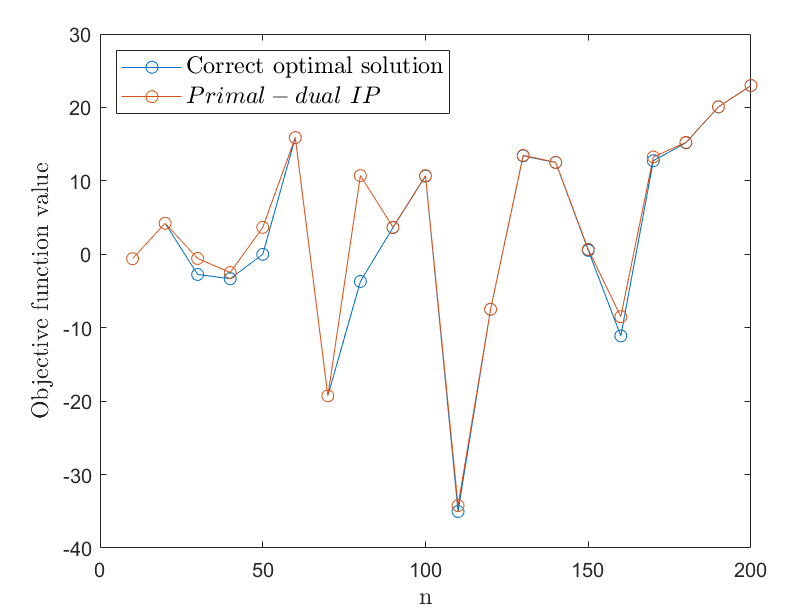
\includegraphics[scale=0.5]{figures/IP_IP_FVAL.PNG}
}
\subfigure[Iteration numbers]{
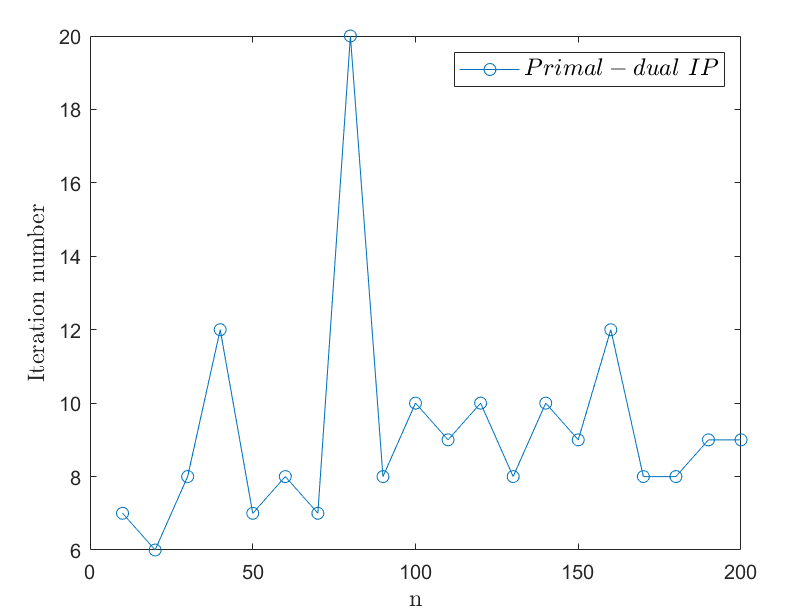
\includegraphics[scale=0.5]{figures/IP_IP_ITERATION.PNG}
}
\caption{Performance of prime-dual interior-point algorithm}
\end{figure}
It can be seen from Figures (a) and (b) that except for when the number of variables is 80($n=80$), the prime-dual interior point method can find a solution very close to the correct optimal solution. It is speculated that when the number of variables is 80, due to the randomness of the parameters in the IP problem, the interior point method encounters a singular matrix problem when solving sub-problems at certain steps, so that the correct solution cannot be obtained. According to Figure c, except for when the number of variables is 80, the prime-dual interior point method maintains a small number of iterations, and can quickly find the optimal solution.
%%%%%%%%%%%%%%%%%%%%%%%%%%%%%%%%%%%%%%%%%%
%%%%%%%%%%%%%%%%%%%%%%%%%%%%%%%%%%%%%%%%%%%
%%%%%%%%%%%%%%%%%%%%%%%%%%%%%%%%%%%%%%%%%%
%%%%%%%%%%%%%%%%%%%%%%%%%%%%%%%%%%%%%%%%%%%
%%%%%%%%%%%%%%%%%%%%%%%%%%%%%%%%%%%%%%%%%%
%%%%%%%%%%%%%%%%%%%%%%%%%%%%%%%%%%%%%%%%%%%
\subsection{\bfseries Primal simplex algorithm}
\begin{shaded}
{Question: Write pseudo-code for a primal simplex algorithm. Explain the algorithm.}
\end{shaded}
{\setmainfont{Times New Roman}\bfseries Pseudo-code}
\begin{algorithm}[!h]
	\caption{Primal simplex algorithm}
	\begin{algorithmic}[1]
	    \STATE Given a basic feasible point $x_0$ and the corresponding index set $\mathcal{B}_0$ and $\mathcal{N}_0$\\
        \WHILE {(not converged)}\\
		\STATE Solve $B^{T} \lambda=g_{B}$ for $\lambda$\\
		\STATE Compute $s_{\mathrm{N}}=g_{\mathrm{N}}-N^{T} \lambda$(pricing)\\
		\IF{($s_N \ge 0$)}\\
		\STATE Stop(optimal point found)\\
		\ENDIF\\
		\STATE Select $q \in \mathcal{N}$ with $s_{q}<0$ as the entering index;\\
		\STATE Solve $B d=A_{q}$ for $d$\\
		\IF{($d \le 0$)}
		\STATE Stop(problem is unbounded)\\
		\ENDIF
		\STATE Calculate $x_{q}^{+}=\min _{i | d_{i}>0}\left(x_{\mathrm{B}}\right)_{i} / d_{i},$ and use $p$ to denote the minimizing $i$\\
		\STATE Update $x_{\mathrm{B}}^{+}=x_{\mathrm{B}}-d x_{q}^{+}, x_{\mathrm{N}}^{+}=\left(0, \ldots, 0, x_{q}^{+}, 0, \ldots, 0\right)^{T}$\\
		\STATE Change $\mathcal{B}$ by adding $q$ and removing the basic variable corresponding to column $p$ of $B$\\
		\ENDWHILE
    \end{algorithmic}
\end{algorithm}\\


Assuming that the matrix $A$ has full column rank, each iterate generated by the simplex method is a basic feasible point of (\ref{con:op4.1}). A
vector $x$ is a basic feasible point if it is feasible and if there exists a subset $\mathcal{B}$ of the index set
$\{1, 2, . . . , n\}$, which called the basis for this problem.\\[0.3cm]
$$B=\left[A_{i}^{\prime}\right]_{i \in \mathcal{B}}\eqno{(4.25)}$$
The basic idea is to start from a vertice of the feasible , and then find the next vertice that makes the objective function smaller from the current vertice along the edge of the feasible polytope, and move to a better one if it can be found for which the basis $\mathcal{B}$ differs. However, another type
of step occurs when the problem is unbounded: The step is an edge along which the objective
function is reduced, and along which iteration point can move infinitely far without ever reaching a
vertex.
The nonbasic matrix is defined as $N=\left[A_{i}^{\prime}\right]_{i \in \mathcal{N}}$ and partition the n-element vectors $x$, $s$, and $g$
according to the index sets $\mathcal{B}$ and $\mathcal{N}$
$$\begin{array}{ll}
x_{\mathrm{B}}=\left[x_{i}\right]_{i \in \mathcal{B}}, & x_{\mathrm{N}}=\left[x_{i}\right]_{i \in \mathcal{N}} \\
s_{\mathrm{B}}=\left[s_{i}\right]_{i \in \mathcal{B}}, & s_{\mathrm{N}}=\left[s_{i}\right]_{i \in \mathcal{N}} \\
g_{\mathrm{B}}=\left[g_{i}\right]_{i \in \mathcal{B}}, & g_{\mathrm{N}}=\left[g_{i}\right]_{i \in \mathcal{N}}
\end{array}$$
From the KKT condition
$$A^{\prime} x=B x_{\mathrm{B}}+N x_{\mathrm{N}}=b\eqno{(4.26)}$$
The primal variable $x$ for this simplex iterate is defined as
$$x_{\mathrm{B}}=B^{-1}b, \qquad x_{\mathrm{N}=0}$$
In order to satisfy the complementarity condition $x_is_i=0$, $ s_{B}=0$ is defined. The remaining components $\lambda$ and $s_N$ can be found by partitioning this condition into $g_B$ and $g_N$
components and using $ s_{B}=0$  to obtain
$$B^{T} \lambda=g_{\mathrm{B}}, \quad N^{T} \lambda+s_{\mathrm{N}}=g_{\mathrm{N}}\eqno{(4.27)}$$
$s_{N}$ can be expressed by $\lambda$
$$s_{\mathrm{N}}=c_{\mathrm{N}}-N^{T} \lambda=c_{\mathrm{N}}-\left(B^{-1} N\right)^{T} c_{\mathrm{B}}\eqno{(4.28)}$$
In order to satisfy the non-negativity of condition$s\ge 0$, To be sure that the $s_B$ certainly satisfy this condition, so if $s_N\ge 0$, an optimal solution can be found. However, there are always one or more of the components of $s_N$ are negative. Then the new index which is one of the indices $q\in \mathcal{N}$ for which $s_q<0$ needs to be chose to enter the basis $\mathcal{B}$. It is called as "entering index"\\[0.3cm]
This process of selecting entering and leaving indices, and performing the algebraic
operations necessary to keep track of the values of the variables $x$, $\lambda$, and $s$, is sometimes
known as pivoting
Then the new iterate $x_B$ updates
$$x_{\mathrm{B}}^{+}=x_{\mathrm{B}}-B^{-1} A_{q}^{\prime} x_{q}^{+}\eqno{(4.29)}$$
It is found that if $d=B^{-1} A_{q}^{\prime}\le 0$, $x_{q}^{+}$ can increase to $\propto$ without ever encountering a new vertex. When this happens, the linear program is unbounded

%%%%%%%%%%%%%%%%%%%%%%%%%%%%%%%%%%%%%%%%%%
%%%%%%%%%%%%%%%%%%%%%%%%%%%%%%%%%%%%%%%%%%%
%%%%%%%%%%%%%%%%%%%%%%%%%%%%%%%%%%%%%%%%%%
%%%%%%%%%%%%%%%%%%%%%%%%%%%%%%%%%%%%%%%%%%%
%%%%%%%%%%%%%%%%%%%%%%%%%%%%%%%%%%%%%%%%%%
%%%%%%%%%%%%%%%%%%%%%%%%%%%%%%%%%%%%%%%%%%%
\subsection{\bfseries Implementation of primal simplex algorithm}
\begin{shaded}
{Question: Implement a primal active-set algorithm (a primal simplex algorithm) for the
linear program. You must provide commented code as well as driver files to
test your code, documentation that it works, and performance statistics.}
\end{shaded}
{\setmainfont{Courier New Bold} \scriptsize            
\begin{lstlisting}
function [x,output]=Pri_Simple(c,A,b,base)
% Pri_Simple  Primal simplex algorithm
%          min  c'*x
%           x
%          s.t. A x  = b      
%               x >= 0   
%         base: base vector
% Syntax: [x,output]=Pri_Simple(c,A,b,base)
%         output.fval: minimum value
%         output.case: 
%                      'found' : optimal solution found
%                      'unbound' : the problem is unbounded
%         output.xarray: Iteration trajectory  
iteration_max=400;
iteration=0;
Xarray=[];
nx=size(A,2);
nc=size(A,1);
%if c>=0 the x can be calculated directly, but only if the constraint is satisfied
if c>=0
    index_c=find(c~=0,1,'last');
    test_c=inv(A(:,(nx-nc+1):nx))*b;
    if test_c>=0
        x=zeros(1,index_c);
        output.fval=0;
    else
        output.case='no optimal point';
        x=NaN;
        output.fval=NaN;
        return;
    end
end
%Initialization of nobasevector
nobase=zeros(1,1);
comp1=1:nx;
count=1;
for i=1:nx
    if(isempty(find(base==comp1(i),1)))
        nobase(count)=i;
        count=count+1;
    end
end
B=A(:,base);
x_B=inv(B)*b;
while(iteration<=iteration_max)
    B=A(:,base);
    N=A(:,nobase);
    c_B = c(base);
    c_N = c(nobase);
    x_B=inv(B)*b;
    
    lambda=inv(B)'*c_B;
    for i=1:length(nobase)
    s_N(i)=c_N(i)-N(:,i)'*lambda;
    end
    [min_q,index_q]=min(s_N);
    %optimal solution found
    if min_q>=0
        output.case='found';
        output.fval=c_B'*x_B;
        index_c=find(c~=0,1,'last');
        for i=1:index_c
            value_c=find(base==i,1);
            if isempty(value_c)
                x(i)=0;
            else
                x(i)=x_B(value_c);
            end
        end
        break;
    end
    %current value
    index_c=find(c~=0,1,'last');
        for i=1:index_c
            value_c=find(base==i,1);
            if isempty(value_c)
                x_tmp(i)=0;
            else
                x_tmp(i)=x_B(value_c);
            end
        end
    x=x_tmp;
    %fprintf("step %d,the current feasible solution is:\n",iteration)
    %fprintf('%.4f, ',x_tmp);
    %fprintf(',\nand the value of z is %.4f\n\n',c_B'*x_B);
    %solve d
    d=inv(B)*A(:,nobase(index_q));
    
    if d<=0
        x=NaN;
        output.fval=NaN;
        output.case='unbounded';
        return;
    end
    %find the leaving indices
    min_xq=inf;
    index_xq=0;
    for i=1:length(d)
        if d(i)>0
            xq=x_B(i)/d(i);
            if xq<min_xq
                min_xq=xq;
                index_xq=i;
            end
        end
    end
    %update the basevector and nobasevector
    tmp=base(index_xq);
    base(index_xq)=nobase(index_q);
    nobase(index_q)=tmp;
    %update x_B
    x_B=x_B-d*min_xq;
    iteration=iteration+1;
    Xarray=[Xarray x_tmp];
end
output.iteration=iteration;
output.xarray=Xarray;
end
\end{lstlisting}}
The same problem is used to test primal simplex algorithm as described in section 4.4. It is shown that the variable values($n$) range from 10 to 200, the curve of deviation expressed by $\left\|x^*-x_{result}\right\|_2$($x^*$ is the correct optimal solution and $x_{result}$ is the optimal solution obtained by the primal simplex algorithm), the curve of the objective function value corresponding to the $x_{*}$ and $x_{result}$ respectively, and the curve of the number of iterations. Please see the driver files in appendix.

\begin{figure}[H]
\centering
\subfigure[Deviation]{
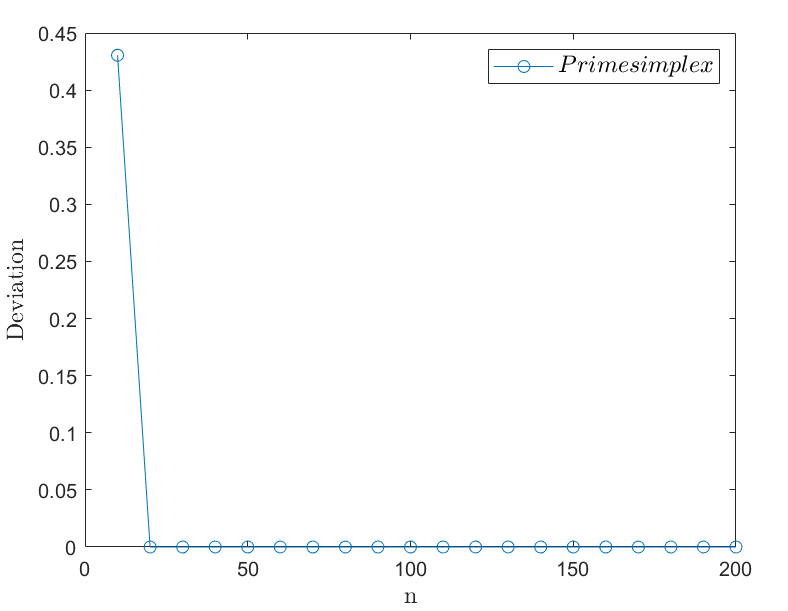
\includegraphics[scale=0.5]{figures/IP_SIMPLEX_NORM.PNG}
%\caption{fig1}
}
\quad
\subfigure[Objective function value]{
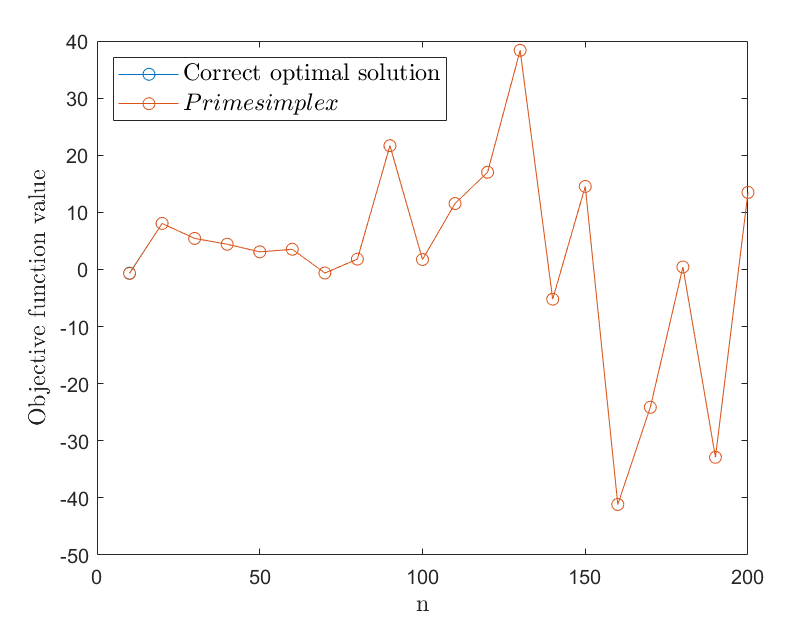
\includegraphics[scale=0.5]{figures/IP_SIMPLEX_FVAL.PNG}
}
\subfigure[Iteration numbers]{
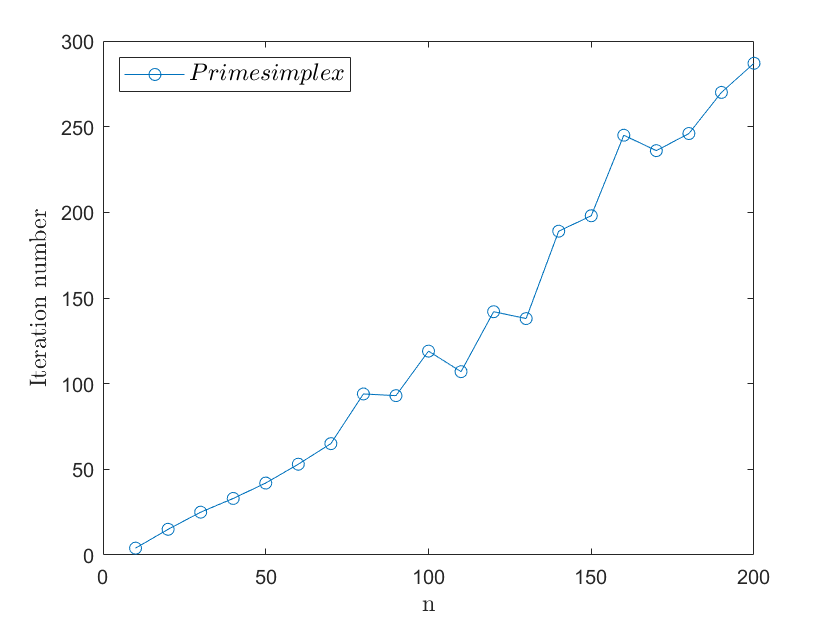
\includegraphics[scale=0.5]{figures/IP_SIMPLEX_ITERATION.PNG}
}
\caption{Performance of primal simplex algorithm}
\end{figure}
It should be noted in Figure b that the objective function value of the correct optimal solution is exactly the same as the value of the optimal value obtained by the simplex method. That is why there is only one curve in figures b. As can be seen from figures a and b, no matter how the number of variables Changes, the simplex method can always find the optimal solution, but at the same time can be seen from Figure c, the number of iterations of the simplex method is gradually increasing.
%%%%%%%%%%%%%%%%%%%%%%%%%%%%%%%%%%%%%%%%%%%%%%%%%%%%%%%%%%%%%%%%%%%%%%%%%%%%%%%%%%%%%%%%%%%%%%%%%%%%%%%%%%%%%%%%%%%%%%%%%%%%%%%%%%%%%%%%%%%%%%%%%%%%%%%%%%%%%%%%%%%%%%%%%%%%%%%%%%%%%%%%%%%%%%%%%%%%%%%%%%%%%%%%%%%%%%%%%%%%%%%%%%%%%%%%%%%%%%%%%%%%%%%%%%%%%%%%%%%%%%%%%%%%%%%%%%%%%%%%%%%%%%%%%%%%%%%%%%%%%%%%%%%%%%%%%%%%%%%%%%%%%%%%%%%%%%%%%%%%%%%%%%%%%%%%%%%%%%%%%%%%%%%%%%%%%%%%%%%%%%%%%%%%%%%%%%%%%%%%%%%%%%%%%%%%%%%%%%%%%%%%%%%%%%%%%%%%%%%%%%%%%%%%%%%%%%%%%%%%%%%%%%%%%%%%%%%%%%%%%%%%%%%%%%%%
\newpage
\subsection{\bfseries Comparison of algorithms}
\begin{shaded}
{Question: Compare the performance of your primal-dual interior-point algorithm, primal
active-set algorithm (primal simplex algorithm), and linprog from Matlab (or
equivalent LP library functions). Provide scripts that demonstrate how you compare the software and comment on the tests and the results.}
\end{shaded}
The same problem is used to test primal simplex algorithm as described in section 4.4. The primal-dual interior-point algorithm, primal simplex algorithm, and linprog("Dual-simplex" is used here) from Matlab are tested. Please see the driver files in appendix \ref{6.4.1}. It is shown that the variable values($n$) range from 10 to 200, the curve of deviation expressed by $\left\|x^*-x_{result}\right\|_2$($x^*$ is the correct optimal solution and $x_{result}$ is the optimal solution obtained by tested three algorithms), the curve of the objective function value corresponding to the $x_{*}$ and $x_{result}$ respectively, and the curve of the number of iterations.
\vspace{-0.5cm}
\begin{figure}[H]
\centering
\setlength{\abovecaptionskip}{-0.2cm} 
\setlength{\belowcaptionskip}{-0.5cm} 
\subfigure[Deviation]{
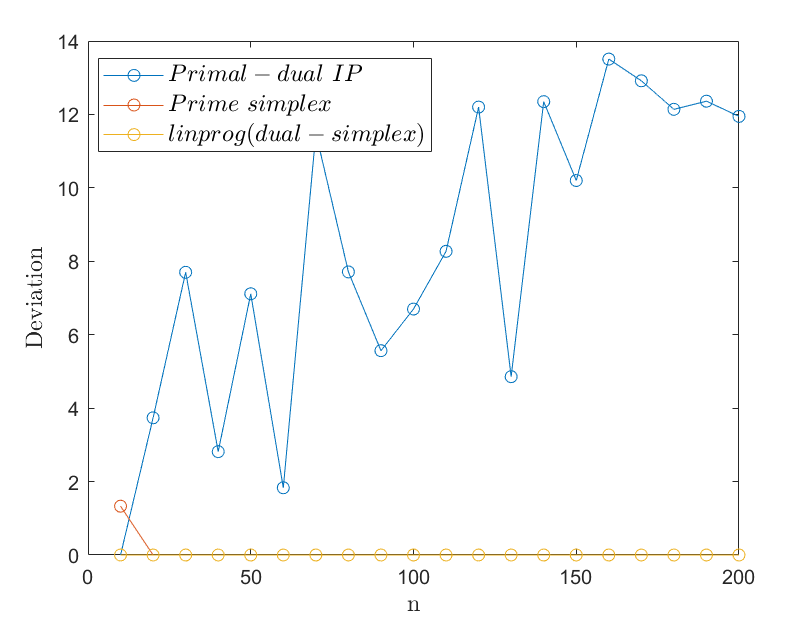
\includegraphics[scale=0.5]{figures/IP_NORM.PNG}
%\caption{fig1}
}
\quad
\subfigure[Objective function value]{
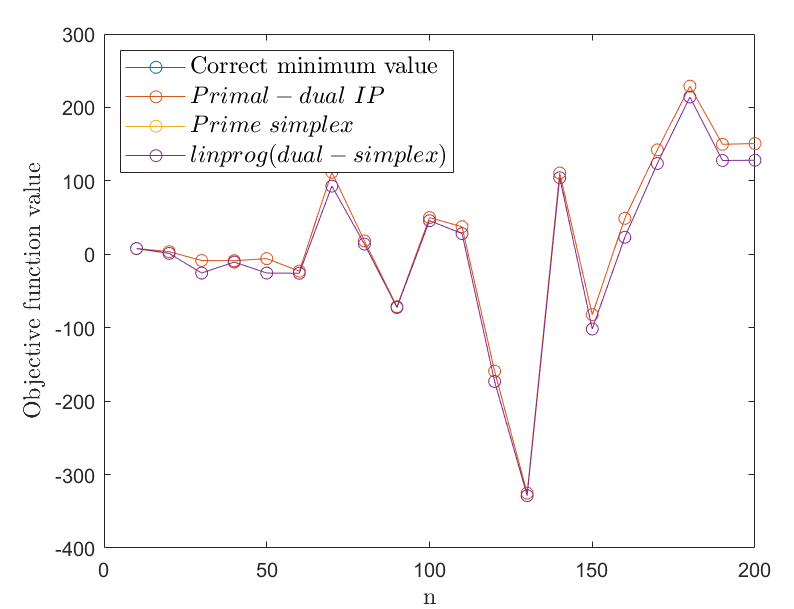
\includegraphics[scale=0.5]{figures/IP_FVAL.PNG}
}
\subfigure[Iteration numbers]{
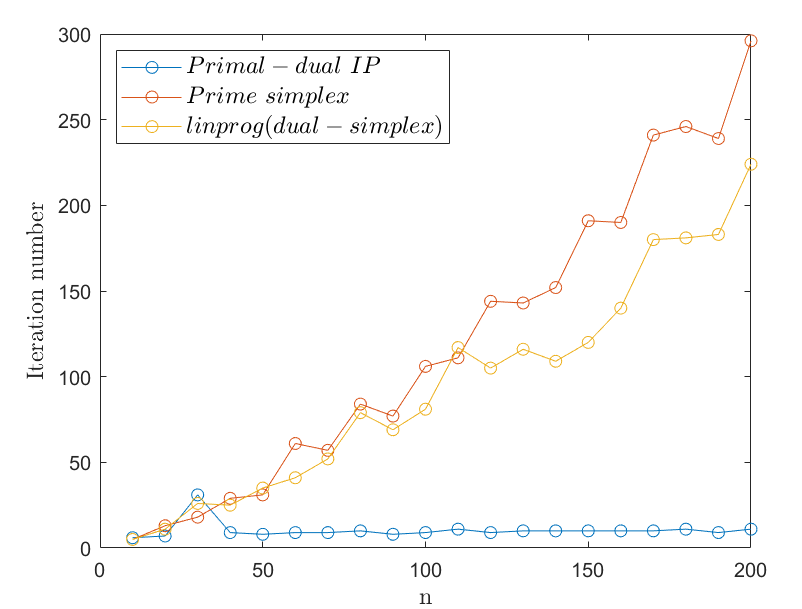
\includegraphics[scale=0.5]{figures/IP_ITERATION.PNG}
}
\caption{Performance of the primal-dual interior-point algorithm, primal simplex algorithm, and linprog("Dual-simplex")}
\end{figure}

Through Figure a, it is found that the test results are consistent with the characteristics of the prime dual interior point method and the simplex method. With the increase in the number of variables, although the interior point method can also approach the correct optimal function, the deviation of the correct optimal solution and found optimal solution will increase larger, but both the prime simplex method implemented and the linprog's dual simplex method can always find the correct optimal solution. This feature can also be verified in Figure b. However, through Figure (c) it can be found that the simplex method can always find the optimal solution at the cost of increasing the number of iterations, which takes more time. The prime-dual interior point method can ensure that the optimal solution can be found in a small number of iterations no matter how many variables are increased.
%%%%%%%%%%%%%%%%%%%%%%%%%%%%%%%%%%%%%%%%%%%%%%%%%%%%%%%%%%%%%%%%%%%%%%%%%%%%%%%%%%%%%%%%%%%%%%%%%%%%%%%%%%%%%%%%%%%%%%%%%%%%%%%%%%%%%%%%%%%%%%%%%%%%%%%%%%%%%%%%%%%%%%%%%%%%%%%%%%%%%%%%%%%%%%%%%%%%%%%%%%%%%%%%%%%%%%%%%%%%%%%%%%%%%%%%%%%%%%%%%%%%%%%%%%%%%%%%%%%%%%%%
 \subsection{\bfseries Markowitz’ portfolio optimization problem as IP}
\begin{shaded}
{Question: Test this on a special Markowitz portfolio optimization problem where we do not
care about risk but just want to maximize the return. Formulate this Markowitz
portfolio optimization problem and test your algorithms. Discuss your tests and
the results. You should solve the problem using your primal-dual interior-point
algorithm, your primal active-set algorithm, and a library algorithm e.g. linprog}
\end{shaded}
Consider a financial market with 5 securities.\\[0.3cm]
\begin{tabular}{c|ccccc|c}
\hline Security & \multicolumn{5}{|c|} { Covariance } &  Return\\
\hline 1 & 2.30 & 0.93 & 0.62 & 0.74 & -0.23 & 15.10 \\
2 & 0.93 & 1.40 & 0.22 & 0.56 & 0.26 & 12.50 \\
3 & 0.62 & 0.22 & 1.80 & 0.78 & -0.27 & 14.70 \\
4 & 0.74 & 0.56 & 0.78 & 3.40 & -0.56 & 9.02 \\
5 & -0.23 & 0.26 & -0.27 & -0.56 & 2.60 & 17.68 \\
\hline
\end{tabular}\\[0.3cm]
The risk is not cared about, so the Linear programming form of Markowitz’ portfolio optimization problem is
\begin{align*}
&\max_{x \in \mathbb{R}^{n}} \quad \phi=x^{\prime} \mu \tag{4.30}\\
& s.t. \quad \sum_{i=1}^{n} x_{i}=1\\
& \quad \quad \ x \ge 0
\end{align*}
Then a portfolio will be computed to obtain maximum of return and the optimal
portfolio, by the primal-dual interior-point algorithm, primal simplex algorithm, and linprog("Dual-simplex" is used here) from Matlab. Please see the driver files in appendix. The result and the iteration numbers are showed\\
The primal-dual interior-point QP algorithm
\begin{align*}
&    x=(0,0,0,0,1)^{\prime}\\
&Return: \quad E\{ R\}=17.68\\
&Iteration=4
\end{align*}
The
primal simplex algorithm
\begin{align*}
&    x=(0,0,0,0,1)^{\prime}\\
&Return: \quad E\{ R\}=17.68\\
&Iteration=1
\end{align*}
The "linprog" with "Dual-simplex"
\begin{align*}
&    x=(0,0,0,0,1)^{\prime}\\
&Return: \quad E\{ R\}=17.68\\
&Iteration=1
\end{align*}
From the same results obtained from the three algorithms, it can be concluded that when risk is not considered, this Markowitz’ portfolio optimization problem can be transformed into a standard linear programming problem only for maximizing returns. The iteration point will eventually iterate to the vertex with the highest return, that is, the fifth security has the highest return of 17.68. At the same time, it is found that in the case where the minimum point is at the constrained vertex, the simplex method finds the optimal value in only one iteration with the help of the movement at the constrained boundary. Although the prime dual interior point method can also approach the minimum point, it requires an additional number of iterations compared to the simplex method.
\newpage
\section{ \bfseries Nonlinear Program (NLP)}
A nonlinear program is considered in the form\\
\begin{align*}
&\min_{x} \quad f(x)\tag{5}\label{con:op5.1}\\
& s.t. \quad g(x)=0\\
& \quad \quad  l\le x \le u
\end{align*}
Assuming that the involved functions are sufficiently smooth for the algorithms discussed in this course to work. Assume that $\nabla_{g(x)}$ has full column rank.
%%%%%%%%%%%%%%%%%%%%%%%%%%%%%%%%%%%%%%%%%%
%%%%%%%%%%%%%%%%%%%%%%%%%%%%%%%%%%%%%%%%%%%%%%%%%%%%%%%%%%%%%%%%%%%%%%%%%%%%%%%%%%%%%
%%%%%%%%%%%%%%%%%%%%%%%%%%%%%%%%%%%%%%%%%%%
%%%%%%%%%%%%%%%%%%%%%%%%%%%%%%%%%%%%%%%%%%
%%%%%%%%%%%%%%%%%%%%%%%%%%%%%%%%%%%%%%%%%%%
\subsection{\bfseries Lagrangian function}
\begin{shaded}
{ Question: What is the Lagrangian function for this problem?}
\end{shaded}
First, the  nonlinear program problem (\ref{con:op5.1}) can be equivalent to the inequailty constrained form

\begin{align*}
&\min_{x} \quad f(x) \tag{5.1}\label{con:op5.2}\\
& s.t. \quad g(x)=0\\
& \quad \quad  h(x)=\begin{bmatrix}
x-l \\ u-x\end{bmatrix}=\left[I\quad -I\right]^{\prime}x+\begin{bmatrix}
-l \\ u\end{bmatrix}\ge 0\Leftrightarrow h(x) \ge 0
\end{align*}\\[0.3cm]
Lagrangian function\\
$$L(x, \mu, \lambda)=f(x)-\mu^{\prime}g(x) -\lambda^{\prime}h(x) \eqno{(5.2)}$$
%%%%%%%%%%%%%%%%%%%%%%%%%%%%%%%%%%%%%%%%%%
%%%%%%%%%%%%%%%%%%%%%%%%%%%%%%%%%%%%%%%%%%%
%%%%%%%%%%%%%%%%%%%%%%%%%%%%%%%%%%%%%%%%%%
%%%%%%%%%%%%%%%%%%%%%%%%%%%%%%%%%%%%%%%%%%%
%%%%%%%%%%%%%%%%%%%%%%%%%%%%%%%%%%%%%%%%%%
%%%%%%%%%%%%%%%%%%%%%%%%%%%%%%%%%%%%%%%%%%%
\newpage
\subsection{\bfseries Necessary optimality conditions}
\begin{shaded}
{Question: What is the necessary first order optimality conditions for the nonlinear program?}
\end{shaded}
First the gradient of the Lagrangian function is
$$\nabla_{x} L(x, \mu, \lambda)=\nabla f(x)-\nabla g(x) \mu-\nabla h(x) \lambda\eqno{(5.3)}$$
From the question it is shown that the $\nabla_{g(x)}$ has full column rank and the inequlity form is $l\le x \le u$ so the assumption of LICQ is valid. Assuming that $\nabla_{g_i(x)}$ and $\nabla_{h_i(x)}$ are linearly independent for all $i \in \mathcal{A}(x)$. \\
The necessary first order optimality conditions\\[0.3cm]
Let $x$ be a local minimizer then
\begin{align*}
    \nabla_{x} L(x, \mu, \lambda)&=\nabla f(x)-\nabla g(x) \mu-\nabla h(x) \lambda=0\tag{5.4}\\
    g(x)&=0\tag{5.5}\\
    h(x)&\ge 0\tag{5.6}\\
    \lambda&\ge 0\tag{5.7}\\
    \lambda h(x)&=0\tag{5.8}
\end{align*}

%%%%%%%%%%%%%%%%%%%%%%%%%%%%%%%%%%%%%%%%%%
%%%%%%%%%%%%%%%%%%%%%%%%%%%%%%%%%%%%%%%%%%%
%%%%%%%%%%%%%%%%%%%%%%%%%%%%%%%%%%%%%%%%%%
%%%%%%%%%%%%%%%%%%%%%%%%%%%%%%%%%%%%%%%%%%%
%%%%%%%%%%%%%%%%%%%%%%%%%%%%%%%%%%%%%%%%%%
%%%%%%%%%%%%%%%%%%%%%%%%%%%%%%%%%%%%%%%%%%%
\subsection{\bfseries Sufficient optimality conditions}
\begin{shaded}
{Question:What are the sufficient second order optimality conditions for the nonlinear program?}
\end{shaded}
First the feasible active direction $h$ is defined. Let $x$ be any feasible point. Then any non-zero vector, $h$, is a feasible active direction if
\begin{align*}
    \nabla g_i(x)^{\prime}h&=0 \qquad \forall i \in \mathcal{A}(x)\tag{5.9}\\
    \nabla h_i(x)^{\prime}h&=0 \quad \text{and} \quad  \lambda_i>0 \qquad \forall i \in \mathcal{A}(x)\tag{5.10}\\
\end{align*}
Then assuming that $(x,\lambda)$ satisfy the first order KKT conditions. If for all feasible active directions, $h \neq 0 $,
$$h^{\prime}\nabla_{xx}^2L(x,\mu,\lambda)h>0\eqno{(5.11)}$$
Then it can be said that the $x$ is a strict local constrained minimizer.
%%%%%%%%%%%%%%%%%%%%%%%%%%%%%%%%%%%%%%%%%%
%%%%%%%%%%%%%%%%%%%%%%%%%%%%%%%%%%%%%%%%%%%
%%%%%%%%%%%%%%%%%%%%%%%%%%%%%%%%%%%%%%%%%%
%%%%%%%%%%%%%%%%%%%%%%%%%%%%%%%%%%%%%%%%%%%
%%%%%%%%%%%%%%%%%%%%%%%%%%%%%%%%%%%%%%%%%%
%%%%%%%%%%%%%%%%%%%%%%%%%%%%%%%%%%%%%%%%%%%
\subsection{\bfseries Description of test problem}
\begin{shaded}
{Question:Choose a specific test problem for a nonlinear program in the form. Present
the problem and argue why you chose this problem.}
\end{shaded}
The Himmelblau Optimization Problem is considered
\begin{align*}
    \min_x \quad &f(x)=\left(x_1^2+x_2-11\right)^2+\left(x_1+x_2^2-7\right)^2\tag{5.12}\\
    &g(x)=\left(x_1+2\right)^2-x_2= 0\\
    &h_1(x)=-x_1+3\ge 0\\
    &h_2(x)=x_2+2\ge 0\\
\end{align*}
There are several reasons to choose the Himmelblau Optimization Problem. First,  the objective function is continuous as required. This function is not convex and has four local minima at 
$$\begin{array}{l}
f\left(\mathbf{x}^{*}\right)=0 \text { at } \mathbf{x}^{*}=(3,2) \\
f\left(\mathbf{x}^{*}\right)=0 \text { at } \mathbf{x}^{*}=(-2.805118,3.283186) \\
f\left(\mathbf{x}^{*}\right)=0 \text { at } \mathbf{x}^{*}=(-3.779310,-3.283186) \\
f\left(\mathbf{x}^{*}\right)=0 \text { at } \mathbf{x}^{*}=(3.584458,-1.848126)
\end{array}$$
Because the SQP algorithm tested is based on iteration, different stating points can be chose to test the optimization results. In order to conveniently present the iterative trajectory of points in the contour, this problem which is defined on the 2-dimensional space is chosen for the test.
The contour of the function is showed here
\begin{figure}[H]
\centering
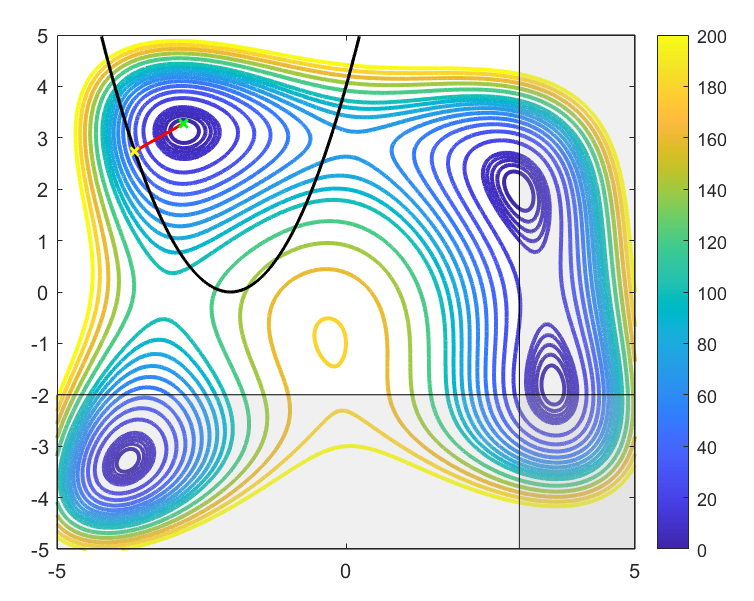
\includegraphics[scale=0.5]{figures/HB_map1.PNG}
\caption{The contour of the function in $x_1\in[-5, 5],x_2\in[-5,5]$}
\label{fig:labe5.4.1}
\end{figure}
A more specific contour under inequality conditions($-x_1+3\ge 0$,$x_2+2\ge 0$)
\begin{figure}[H]
\centering
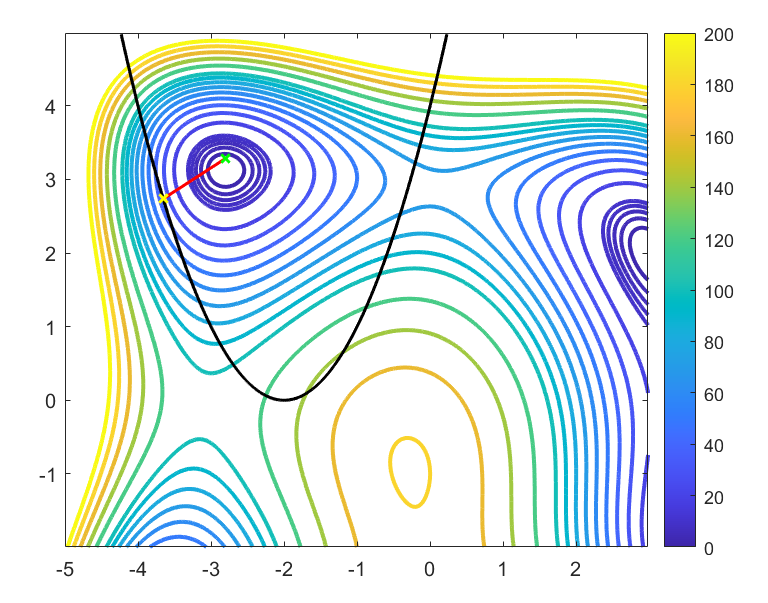
\includegraphics[scale=0.5]{figures/HB_map_ieq.PNG}
\caption{The contour of the function in $x_1\in[-5, 3],x_2\in[-2,5]$}
\label{fig:labe5.4.2}
\end{figure}
The black curve is the equality constraint $\left(x_1+2\right)^2-x_2= 0$, and one of the two ends of the red line is the minimum point($-2.8051,3.2832$) of the objective equation without constraints, corresponding to the green $\times$, and the other is the minimum point($-3.6546,2.7377$) under the constraints of the equations and inequalities of this problem, corresponding to the yellow $\times$.

%%%%%%%%%%%%%%%%%%%%%%%%%%%%%%%%%%%%%%%%%%
%%%%%%%%%%%%%%%%%%%%%%%%%%%%%%%%%%%%%%%%%%%
%%%%%%%%%%%%%%%%%%%%%%%%%%%%%%%%%%%%%%%%%%
%%%%%%%%%%%%%%%%%%%%%%%%%%%%%%%%%%%%%%%%%%%
%%%%%%%%%%%%%%%%%%%%%%%%%%%%%%%%%%%%%%%%%%
%%%%%%%%%%%%%%%%%%%%%%%%%%%%%%%%%%%%%%%%%%%
\subsection{\bfseries Solution to the problem by fmincon}
\begin{shaded}
{Question:Solve the test problem using a library function for nonlinear programs, e.g. fmincon in Matlab.}
\end{shaded}
First, it is necessary to respectively construct the function that outputs the objective function and his gradient, and the function that outputs the equality and inequality constraints and his gradient.\\[0.3cm]
For objective function and his gradient
\begin{align*}
    f(x_1,x_2)&=\left(x_1^2+x_2-11\right)^2+\left(x_1+x_2^2-7\right)^2\\
    \nabla f(x)&=\left[\begin{array}{l}
4 x_{1}\left(x_{1}^{2}+x_{2}-11\right)+2\left(x_{1}+x_{2}^{2}-7\right) \\
2\left(x_{1}^{2}+x_{2}-11\right)+4 x_{2}\left(x_{1}+x_{2}^{2}-7\right)
\end{array}\right]\tag{5.13}
\end{align*}
{\setmainfont{Courier New Bold} \scriptsize         
\begin{lstlisting}
function [f,dfdx]=objfunHimmelblau(x,p)
tmp1=x(1)*x(1)+x(2)-11;
tmp2=x(1)+x(2)*x(2)-7;
f=tmp1*tmp1+tmp2*tmp2;

%compute gradient
if nargout>1
    dfdx=zeros(2,1);
    dfdx(1,1)=4*tmp1*x(1)+2*tmp2;
    dfdx(2,1)=2*tmp1+4*tmp2*x(2);
end
\end{lstlisting}}
For equality constraints and its gradient
\begin{align*}
c_1(x_1,x_2)&=\left(x_1+2\right)^2-x_2\\
\nabla c_1(x)&=\left[\begin{array}{c}
2\left(x_{1}+2\right) \\
-1
\end{array}\right]\tag{5.14}
\end{align*}
{\setmainfont{Courier New Bold} \scriptsize         
\begin{lstlisting}
function [c,ceq,dcdx,dceqdx]=confunHimmeblau(x,p)
c=zeros(0,1);
ceq=zeros(1,1);
%c<=0  
x1=x(1,1);
x2=x(2,1);
tmp=x1+2;
%Equality constraint 
ceq=tmp^2-x2;

% computer constraint gradients
if nargout>2
    dcdx=zeros(2,0);
    dceqdx=zeros(2,1);
    %Gradient of Equality constraint
    dceqdx(1,1)=2*tmp;
    dceqdx(2,1)=-1;
end
\end{lstlisting}}
Four starting points that are located on the left A=($-5,3$), below B=($-2,-2$), right C=($3,3$), and above D=($-2,5$) of the equality constraint curve (position in the figure) and at inequality constraint and the intersection E=($3,-2$) of two inequality constraints are selected . Please see the driver files in Appendix \ref{6.5.1}, \ref{6.5.2} and \ref{6.5.3}. The SQP algorithm and interior-point algorithm are both tested by fmincon, and the result is 
\begin{table}[!htbp]
\centering
\begin{tabular}{|c|c|c|c|c|c|}
\hline
&A($-5,3$)&B($-2,-2$)&C($3,3$)&D($-2,5$)&E($3,-2$)\\
\hline
SQP&($-3.65,2.73$)&($-3.65,2.73$)&($-0.29,2.89$)&($-3.65,2.73$)&($-0.29,2.89$)\\
\hline
Interior-point&($-3.65,2.73$)&($-3.65,2.73$)&($-0.29,2.89$)&($-3.65,2.73$)&($-0.29,2.89$)\\
\hline
\end{tabular}
\end{table}
$$\begin{array}{l}
f\left(\mathbf{x}^{*}\right)=65.43 \text { at } \mathbf{x}^{*}=(-0.29,2.89) \\
f\left(\mathbf{x}^{*}\right)=35.93 \text { at } \mathbf{x}^{*}=(-3.65,2.73) \\
\end{array}$$
It is found that whether the algorithm SQP or Interior-point in the fmincon function is used, the minimum value obtained for the same starting point is the same. It can be seen that starting points $A$, $B$, and $D$ have reached the correct minimum points, but starting points $C$ and $E$ reached a sub-minimum point.\\
First iterative trajectory of starting points $C$ and $E$ in the contour is showed 
\begin{figure}[H]
\centering
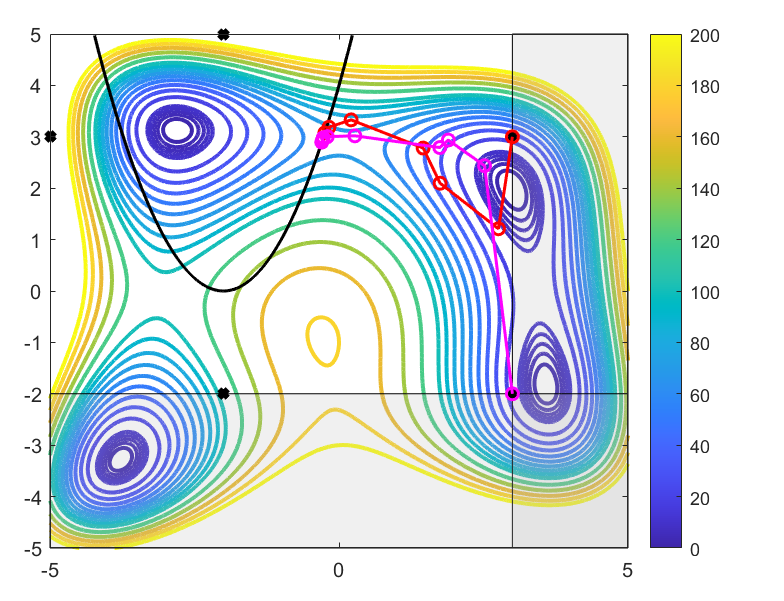
\includegraphics[scale=0.5]{figures/fmincon_CE.PNG}
\caption{Iterative trajectory of starting points $C$ and $E$}
\label{fig:labe5.4.3}
\end{figure}
It is found that because there is a maximum value in the lower part of the equation constraint curve, when the starting point is on the right side of the equation constraint curve, the iteration point will not cross the maximum value area, but in the right half of the equation constraint curve to search for the minimum point. As a result, the correct minimum value cannot be found in the left half of the equality constraint, but can only reach the sub-minimum value.
Iterative trajectory of starting points $A$, $B$, and $D$ in the contour is showed 
\begin{figure}[H]
\centering
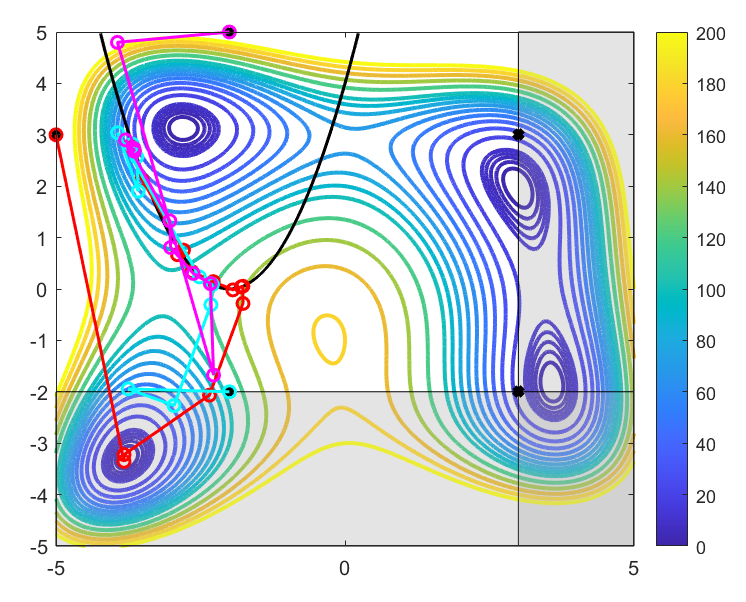
\includegraphics[scale=0.5]{figures/fmincon_ABD.PNG}
\caption{Iterative trajectory of starting points $A$, $B$, and $D$}
\label{fig:labe5.4.4}
\end{figure}
When the starting point is not obstructed by the area where the maximum value is, the correct minimum point can be found.
%%%%%%%%%%%%%%%%%%%%%%%%%%%%%%%%%%%%%%%%%%
%%%%%%%%%%%%%%%%%%%%%%%%%%%%%%%%%%%%%%%%%%%
%%%%%%%%%%%%%%%%%%%%%%%%%%%%%%%%%%%%%%%%%%
%%%%%%%%%%%%%%%%%%%%%%%%%%%%%%%%%%%%%%%%%%%
%%%%%%%%%%%%%%%%%%%%%%%%%%%%%%%%%%%%%%%%%%
%%%%%%%%%%%%%%%%%%%%%%%%%%%%%%%%%%%%%%%%%%%
\newpage
\subsection{\bfseries SQP algorithm with damped BFGS}
\begin{shaded}
{Question:Explain, discuss and implement an SQP procedure with a damped BFGS approximation to the Hessian matrix for the problem. Make a table with the iteration sequence for different starting points. Plot the iteration sequence in a
contour plot. Discuss the results.}
\end{shaded}
First, the KKT conditions of this nonlinear problem are considered
\begin{align*}
\nabla_x L(x,\mu,\lambda)&=\nabla f(x)-\nabla g(x)\mu-\nabla h(x) \lambda=0\tag{5.15}\\
\nabla_{\mu} L(x,\mu,\lambda)&=-g(x)=0\tag{5.16}\\
\nabla_{\lambda} L(x,\mu,\lambda)&=-h(x)\le 0\tag{5.17}
\end{align*}
Newton's method 

$$\left[\begin{array}{cc}
\nabla_{x x}^{2} L\left(x_{k}, \mu_{k}, \lambda_{k}\right) & -\nabla g\left(x_{k}\right) \\
-\nabla g\left(x_{k}\right)^{\prime} & 0
\end{array}\right]\left[\begin{array}{c}
\Delta x \\
\Delta \mu
\end{array}\right]=-\left[\begin{array}{c}
\nabla_{x} L\left(x_{k}, \mu_{k}, \lambda_{k}\right) \\
-g\left(x_{k}\right)
\end{array}\right]\eqno{(5.18)}$$\\
$$\left[-\nabla h(x_k)^{\prime}\right]\left[\Delta \lambda\right]\le -\left[-h(x_k)\right]\eqno{(5.19)}$$
The assumption is noted that first the constraint Jacobian $\nabla g(x_k)$ has full column rank, and the matrix $L\left(x_{k}, \mu_{k}, \lambda_{k}\right) & -\nabla g\left(x_{k}\right)$ is positive definite on the tangent space of the constraints, that is, $d^{\prime}L\left(x_{k}, \mu_{k}, \lambda_{k}\right) & -\nabla g\left(x_{k}\right)d> 0$ for all $d\noq 0$ such that $\nabla dg(x_k)=0$
Then a subproblem which is a quadratic programming problem can be constructed
$$\begin{aligned}
\min _{\Delta x \in \mathbb{R}^{n}} \qquad & \frac{1}{2} \Delta x^{\prime}\left[\nabla_{x x}^{2} L\left(x_{k}, \mu_{k},\lambda_{k}\right)\right] \Delta x+\left[\nabla_{x} L\left(x_{k}, \mu_{k},\lambda_{k}\right)\right]^{\prime} \Delta x \\
\text {s.t.} \qquad & \nabla g\left(x_{k}\right)^{\prime} \Delta x=-g\left(x_{k}\right)\\
& \nabla h\left(x_{k}\right)^{\prime} \Delta x\ge -h\left(x_{k}\right)
\end{aligned}\eqno{(5.20)}$$
Which can be expressed as
$$\begin{aligned}
\min _{\Delta x \in \mathbb{R}^{n}} \qquad & \frac{1}{2} \Delta x^{\prime}H\Delta x+g^{\prime}\Delta x \\
\text {s.t.} \qquad & A^{\prime} \Delta x=b\\
& C^{\prime} \Delta x=d
\end{aligned}\eqno{(5.21)}$$
with
$$\begin{array}{lll}
H=\nabla_{x x}^{2} L\left(x_{k}, \mu_{k},\lambda_{k}\right) & g=\nabla f\left(x_{k}\right)\\
A=\nabla g\left(x_{k}\right) & b=-h\left(x_{k}\right)\\
C=\nabla g\left(x_{k}\right) & d=-h\left(x_{k}\right)
\end{array}$$
The Hessian matrix of the nonlinear function is always hard to compute, so the damped BFGS approximation to the Hessian matrix is always used. The idea is to update a $B_k$ to replace the $H$, where the vectors $s_k$ and $y_k$ are defined as 
\begin{align*}
    s_k&=x_{k+1}-x_k\tag{5.22}\\
    y_k&=\nabla_{x} L\left(x^{k+1},\mu^{k+1},\lambda^{k+1}\right)-\nabla_{x}L\left(x^{k}, \mu^{k+1},\lambda^{k+1}\right)\tag{5.23}
\end{align*}
Given a symmetric and positive definite matrix $B_k$\\
Defined $r_k$ as
$$r_{k}=\theta_{k} y_{k}+\left(1-\theta_{k}\right) B_{k} s_{k}\eqno{(5.24)}$$
Where the scalar $\theta_{k}$ is defined as
$$\theta_{k}=\left\{\begin{array}{ll}
1 & \text {if } s_{k}^{\prime} y_{k} \geq 0.2 s_{k}^{\prime} B_{k} s_{k} \\
\left(0.8 s_{k}^{\prime} B_{k} s_{k}\right) /\left(s_{k}^{\prime} B_{k} s_{k}-s_{k}^{\prime} y_{k}\right) & \text { if } s_{k}^{\prime} y_{k}<0.2 s_{k}^{\prime} B_{k} s_{k}
\end{array}\right\eqno{(5.25)}$$
Update $B_k$ as follows
$$B_{k+1}=B_{k}-\frac{B_{k} s_{k} s_{k}^{\prime} B_{k}}{s_{k}^{\prime} B_{k} s_{k}}+\frac{r_{k} r_{k}^{\prime}}{s_{k}^{\prime} r_{k}}\eqno{(5.26)}$$
From the updating with $r_k$ replaced by $r_k$. It guarantees that $B_{k+1}$ is positive definite.

{\setmainfont{Times New Roman}\bfseries Pseudo-code}
\begin{algorithm}[H]
	\caption{ SQP algorithm with damped BFGS}
	\begin{algorithmic}[1]
	    \STATE Given a starting point($x_0,\mu_0,\lambda_0$), set $k=0$\\
		\STATE Evaluate $f_0,\nabla f_0,g_0,\nabla g_0,h_0,\nabla h_0$\\
		\STATE Choose an initial $n \times n$ symmetric positive definite Hessian approximation $B_0$, always an Identity matrix\\
        \WHILE {(not converged)}\\
		\STATE Compute the $p_k$($\Delta x_k$),$\mu_{k+1}$ and $\lambda_{k+1}$by solving the sub-quadratic-problem\\
		\STATE Compute $x_{k+1}=x_k+p_k$\\
		\STATE Compute $\nabla_{x}L\left(x_{k}, \mu_{k+1},\lambda_{k+1}\right)=\nabla f(x_k)-\nabla g(x_k)\mu_{k+1}-\nabla h(x_k)\lambda_{k+1}$\\
		\STATE Evaluate $f_{k+1},\nabla f_{k+1},g_{k+1},\nabla g_{k+1},h_{k+1},\nabla h_{k+1}$\\
		\STATE Compute $\nabla_{x}L\left(x_{k+1}, \mu_{k+1},\lambda_{k+1}\right)=\nabla f(x_{k+1})-\nabla g(x_{k+1})\mu_{k+1}-\nabla h(x_{k+1})\lambda_{k+1}$\\
		\STATE Compute the $s_k$ and $y_k$\\
		\STATE Update the Hessian matrix by the modified BFGS procedure\\
		\STATE $k=k+1$\\
		\ENDWHILE
    \end{algorithmic}
\end{algorithm}
Next the specific Matlab code of implementation is showed. The function "Hg_f" which calculate the gradients and hessian of object-function and itself, the "Hg_ceq" which calculate the gradients and hessian of equality constraints and itself, the "Hg_ciq" which calculate the gradients and hessian of equality constraints and itself ,the "Qpsolver_Sqp" which solve the sub-problem of SQP algorithm are stated in appendix \ref{6.5.4}, \ref{6.5.5}, \ref{6.5.6} and \ref{6.5.7}. Only the main program is showed here\\

{\setmainfont{Courier New Bold} \scriptsize         
\begin{lstlisting}
function [x,output]=Sqp_Bfgs(x0,lam_eq0,lam_ineq0)
% Sqp_Bfgs  SQP algorithm with damped BFGS and line search
%
%          min  f(x)
%           x
%          s.t. ceq(x)=0  (Lagrange multiplier lam_eq)    
%               ciq(x)>=0  (Lagrange multiplier lam_ineq)  
% Syntax: [x,output]=Sqp_Bfgs(x0,lam_eq0,lam_ineq0)
%         output.fval: minimum value
%         output.dL: convergence of delta_L
%         output.ceq: convergence of ceq
%         output.Xarray=Xarray: Iteration trajectory  
epsilon=1e-6;

Xarray=[];
normdLarray=[];
normceqarray=[];
Xarray=[Xarray x0];

nx=size(x0,1);
Bk=eye(nx);
%evaluate the gradient
[~,df,~]=Hg_f(x0);
[ceq,dceq,~]=Hg_ceq(x0);
[ciq,dciq,~]=Hg_ciq(x0);
xk=x0;
lam_eqk=lam_eq0;
lam_ineqk=lam_ineq0;
iteration=0;
iteration_max=200;
while(iteration<iteration_max)
    %Solve the subproblem(QP)
    [p,lameq,lamineq]=Qpsolver_Sqp(Bk,df,dceq,ceq,dciq,ciq);
    %Take step and update x(k+1),lameq(k+1),lamineq(k+1)
    xk=xk+p;
    lam_eqk=-lameq;
    lam_ineqk=-lamineq;
    %Calculate dL(k) with x(k) and lameq(k+1),lamineq(k+1)
    Lk=df-dceq.*lam_eqk-dciq*lam_ineqk;
    %Re-evaluate
    [~,df,~]=Hg_f(xk);
    [ceq,dceq,~]=Hg_ceq(xk);
    [ciq,dciq,~]=Hg_ciq(xk);
    %Calculate L(k+1) with x(k+1) and lam(k+1)
    Lk2=df-dceq.*lam_eqk-dciq*lam_ineqk;
    %Damped BFGS update
    pk=p;
    qk=Lk2-Lk;
    judge=(pk'*qk>=0.2*pk'*(Bk*pk));
    thetak=judge.*1+(~judge).*((0.8*pk'*(Bk*pk))/(pk'*(Bk*pk)-pk'*qk));
    rk=thetak*qk+(1-thetak)*(Bk*pk);
    Bk=Bk-((Bk*pk)*(pk'*Bk))/(pk'*(Bk*pk))+(rk*rk')/(pk'*rk);
    %Check teh convergence
    if ((norm(Lk2,"inf")<epsilon)&&(norm(ceq,"inf")<epsilon)&&(max(abs(ciq)) + epsilon >= 0)...
       &&(min(lam_ineqk) + epsilon >= 0))
        break;
    end
    iteration=iteration+1;
    Xarray=[Xarray xk];
    normdLarray=[normdLarray norm(Lk2,"inf")];
    normceqarray=[normceqarray norm(ceq,"inf")];
end
[fval,~,~]=Hg_f(xk);
x=xk;
output.fval=fval;
output.xarray=Xarray;
output.dL=normdLarray;
output.ceq=normceqarray;
output.iteration=iteration;
end
\end{lstlisting}}
The algorithm will be tested with the same initial
points as in the section 5.5. Please see the test code in Appendix \ref{6.5.8}. Iterative trajectory of starting points $A$, $B$, $C$, $D$ and $E$ in the contour is showed 

\begin{figure}[H]
\centering
\setlength{\abovecaptionskip}{0cm} 
\setlength{\belowcaptionskip}{-0.5cm}
\subfigure[$A(-5,3)$]{
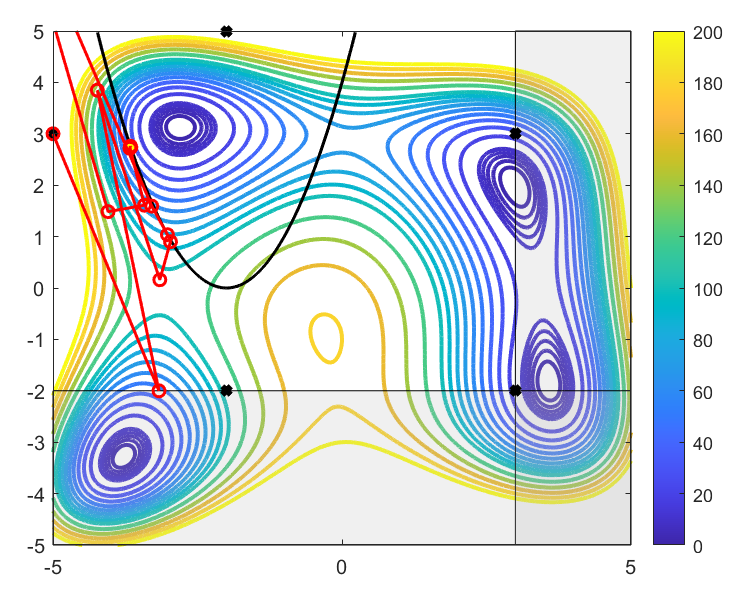
\includegraphics[scale=0.4]{figures/SQP_BFGS_A.PNG}
%\caption{fig1}
}
\quad
\subfigure[$B(-2,-2)$]{
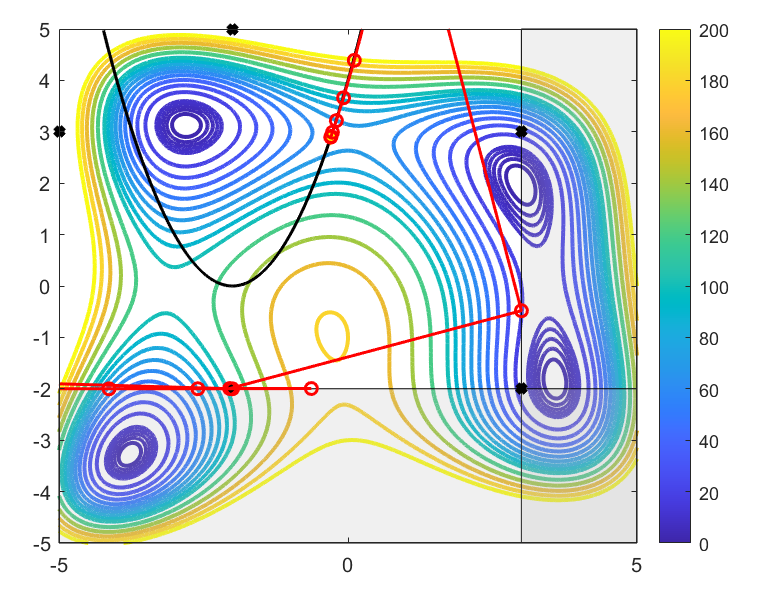
\includegraphics[scale=0.4]{figures/SQP_BFGS_B.PNG}
}
\quad
\subfigure[$C(3,3)$]{
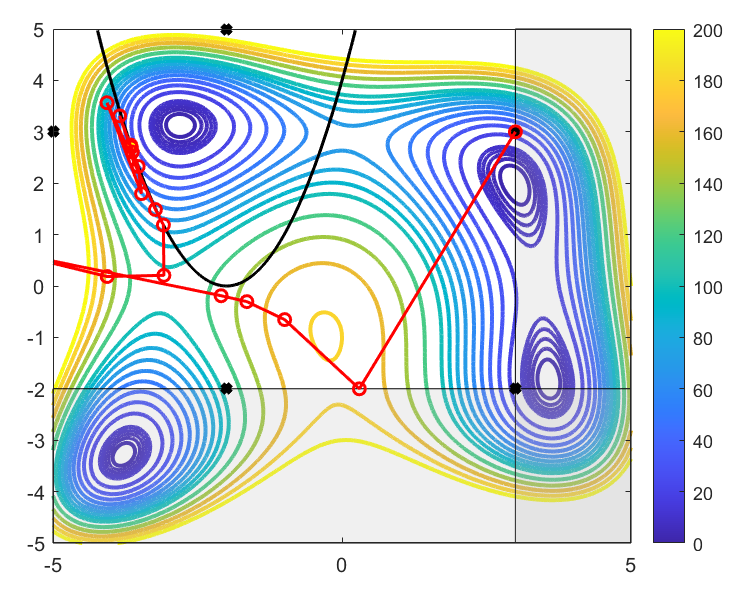
\includegraphics[scale=0.4]{figures/SQP_BFGS_C.PNG}
}
\quad
\subfigure[$D(-2,5)$]{
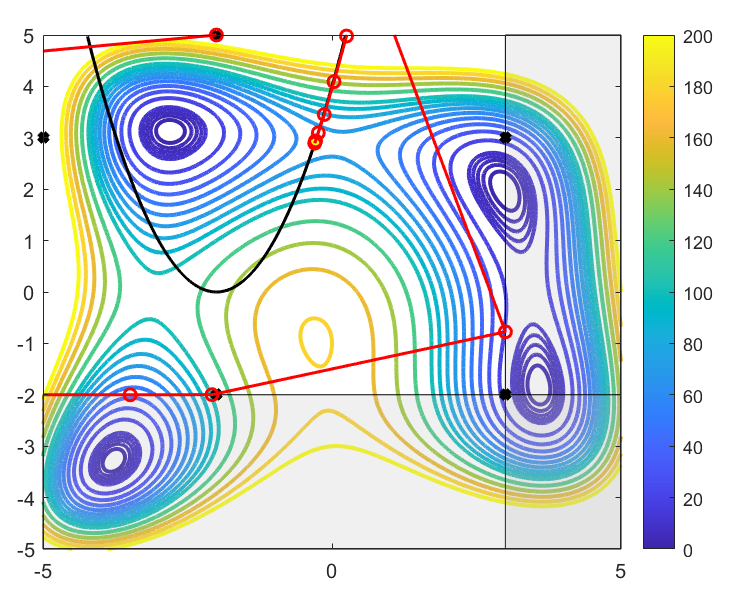
\includegraphics[scale=0.4]{figures/SQP_BFGS_D.PNG}
}
\quad
\subfigure[$E(3,-2)$]{
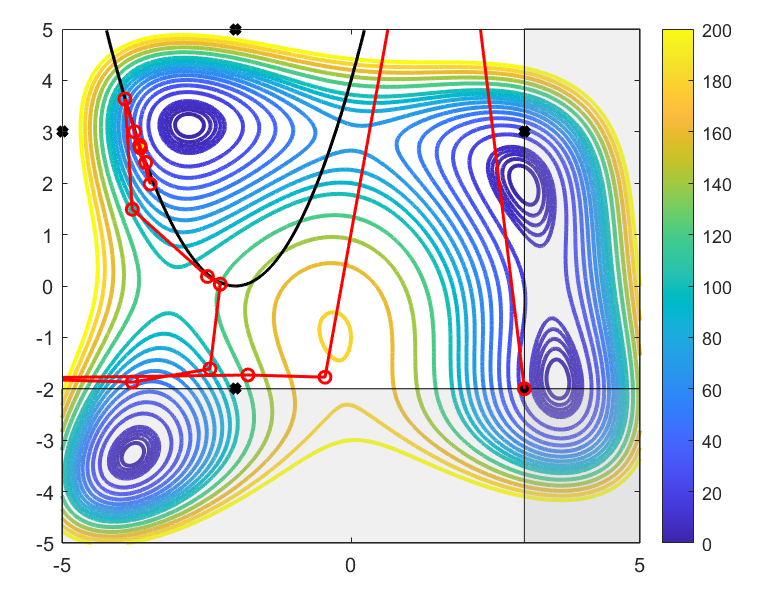
\includegraphics[scale=0.4]{figures/SQP_BFGS_E.PNG}
}
\caption{ Iterative trajectory in contour}
\end{figure}
%%%%%%%%%%%%%%%%%%%%%%%%%%%%%%%%%%%%%%%%%%%%%%%%%%%%%%%
The iteration of table is showed here separately
%%%%%%%%%%%%%%%%%%%%%%%%%%%%%%%%%%%%%%%%%%%%%%%%%%%%%%
\begin{table}[H]
\centering
\setlength{\abovecaptionskip}{0cm} 
\setlength{\belowcaptionskip}{-0.5cm}
\scriptsize
\begin{tabular}{|c|c|c|c|c|c|c|c|c|c|c|}
\hline
$x_0=A(-5,3)$&0&1&2&3&4&5&6&7&8&9\\
\hline
$x_1$&-5.0 & -3.17 & -4.23 & -3.15 & -2.97 & -3.02 & -3.29 & -5.69 & -4.05& -3.42\\
\hline
$x_2$&3.0 & -2.0 & 3.85 & 0.16 & 0.901 & 1.04 & 1.59 & 7.87 & 1.49 & 1.61
\\
\hline
\end{tabular}
\begin{tabular}{|c|c|c|c|c|}
\hline
$x_0=A(-5,3)$&10&11&12&13\\
\hline
$x_1$ & -3.67 & -3.66 & -3.65 & -3.65\\
\hline
$x_2$ & 2.72 & 2.76 & 2.73 & 2.74
\\
\hline

\end{tabular}
\caption{$x_0=A(-5,3)$}
\end{table}

%%%%%%%%%%%%%%%%%%%%%%%%%%%%%%%%%%%%%%%%%%%%%%%%%%%%%%%%%
\begin{table}[H]
\centering
\setlength{\abovecaptionskip}{0cm} 
\setlength{\belowcaptionskip}{-0.5cm} 
\scriptsize
\begin{tabular}{|c|c|c|c|c|c|c|c|c|c|c|}
\hline
$x_0=B(-2,-2)$&0&1&2&3&4&5&6&7&8&9\\
\hline
$x_1$&-2.0 & -64.0 & -33.0 & -21.3 & -11.6 & -6.69 & -4.13 & -2.6 & -0.635 & -2.05 \\
\hline
$x_2$&-2.0 & 0 & -2.0 & 236.0 & -2.0 & -2.0 & -2.0 & -2.0 & -1.99 & -1.99    
\\
\hline
\end{tabular}

\begin{tabular}{|c|c|c|c|c|c|c|c|c|c|c|}
\hline
$x_0=B(-2,-2)$&10&11&12&13&14&15&16&17&18&19\\
\hline
$x_1$&3.0 & 1.22 & 0.972 & 0.955 & 0.902 & 0.663 & 0.347 & 0.109 & -0.0775 & -0.202   \\
\hline
$x_2$&-0.481 & 7.22 & 8.77 & 8.73 & 8.42 & 7.03 & 5.41 & 4.39 & 3.66 & 3.22
\\
\hline
\end{tabular}

\begin{tabular}{|c|c|c|c|c|C|}
\hline
$x_0=B(-2,-2)$&20&21&22&23&24\\
\hline
$x_1$&-0.269 & -0.294 & -0.298 & -0.298 & -0.298  \\
\hline
$x_2$& 2.99 & 2.91 & 2.9 & 2.9 & 2.9
\\
\hline
\end{tabular}
\caption{$x_0=B(-2,-2)$}
\end{table}
%%%%%%%%%%%%%%%%%%%%%%%%%%%%%%%%%%%%%%%%%%%%%%%%%%%%%%%%%%%%%
\begin{table}[H]
\centering
\setlength{\abovecaptionskip}{0cm} 
\setlength{\belowcaptionskip}{-0.5cm}
\scriptsize
\begin{tabular}{|c|c|c|c|c|c|c|c|c|c|c|}
\hline
$x_0=C(3,3)$&0&1&2&3&4&5&6&7&8&9\\
\hline
$x_1$&3.0 & 0.3 & -0.992 & -1.65 & -2.09 & -6.08 & -4.06 & -3.08 & -3.09 & -3.23 \\
\hline
$x_2$&3.0 & -2.0 & -0.654 & -0.304 & -0.189 & 0.737 & 0.184 & 0.208 & 1.19 & 1.49
\\
\hline
\end{tabular}
\begin{tabular}{|c|c|c|c|c|c|c|c|c|c|}
\hline
$x_0=C(3,3)$&10&11&12&13&14&15&16&17&18\\
\hline
$x_1$ &-4.07 & -3.47 & -3.53 & -3.85 & -3.63 & -3.64 & -3.66 & -3.65 & -3.65\\
\hline
$x_2$ & 3.57 & 1.8 & 2.33 & 3.31 & 2.61 & 2.7 & 2.74 & 2.74 & 2.74
\\
\hline

\end{tabular}
\caption{$x_0=C(3,3)$}
\end{table}
%%%%%%%%%%%%%%%%%%%%%%%%%%%%%%%%%%%%%%%%%%%%%%%%%%%%%%%%%%%%%%%
\begin{table}[H]
\centering
\scriptsize
\begin{tabular}{|c|c|c|c|c|c|c|c|c|c|c|}
\hline
$x_0=D(-2,5)$&0&1&2&3&4&5&6&7&8&9\\
\hline
$x_1$&-2.0 & -50.0 & -26.0 & -16.9 & -9.37 & -5.55 & -3.49 & -2.08 & 3.0 & 1.02  \\
\hline
$x_2$&5.0 & 0 & -2.0 & 138.0 & -2.0 & -2.0 & -2.0 & -2.0 & -0.774 & 5.18 
\\
\hline
\end{tabular}
\begin{tabular}{|c|c|c|c|c|c|c|c|c|c|c|c|}
\hline
$x_0=D(-2,5)$&10&11&12&13&14&15&16&17&18&19&20\\
\hline
$x_1$ &0.652 & 0.622 & 0.551 & 0.252 & 0.0345 & -0.134 & -0.237 & -0.285 & -0.297 & -0.298    & -0.298\\
\hline
$x_2$& 6.9 &6.88 & 6.5 & 4.98 & 4.09 & 3.45 & 3.1 & 2.94 & 2.9 & 2.9     & 2.9
\\
\hline

\end{tabular}
\caption{$x_0=D(-2,5)$}
\end{table}
%%%%%%%%%%%%%%%%%%%%%%%%%%%%%%%%%%%%%%%%%%%%%%%%%%%%%%%%%%%
\begin{table}[H]
\centering
\setlength{\abovecaptionskip}{0cm} 
\setlength{\belowcaptionskip}{-0.5cm}
\scriptsize
\begin{tabular}{|c|c|c|c|c|c|c|c|c|c|c|}
\hline
$x_0=E(3,-2)$&0&1&2&3&4&5&6&7&8&9\\
\hline
$x_1$&3.0 & 1.59 & -0.45 & -1.78 & -6.03 & -3.78 & -2.44 & -2.26 & -2.48 & -3.78  \\
\hline
$x_2$&-2.0 & 10.9 & -1.77 & -1.73 & -1.79 & -1.87 & -1.61 & 0.0366 & 0.185 & 1.49  
\\
\hline
\end{tabular}
\begin{tabular}{|c|c|c|c|c|c|c|c|c|}
\hline
$x_0=E(3,-2)$&10&11&12&13&14&15&16&17\\
\hline
$x_1$ &-3.91 & -3.47 & -3.55 & -3.74 & -3.64 & -3.65 & -3.65 & -3.65\\
\hline
$x_2$&  3.64 & 1.98 & 2.4 & 3.0 & 2.68 & 2.73 & 2.74 & 2.74
\\
\hline

\end{tabular}
\caption{$x_0=E(3,-2)$}
\end{table}
It can be seen that starting points $A$, $C$, and $E$ have reached the correct minimum points, but starting points $B$ and $D$ reached a sub-minimum point.\\
When analyze the results solved by fmincon, it is inferred that the staring points $C$ and $E$ which located on the right side of the equation constraint curve cannot cross the area where the maximum value is located, and they can only enter the right half of the equation constraint curve to find the sub-minimum point. However, in the results of this algorithm, it is found that the right point can cross the area where the maximum value is located, and find the minimum point in the left half of the equation constraint curve. It is inferred that this is related to the step size being too large. At some steps, the step size is directly taken as the solution of the sub-problem, so some iteration process steps are too large, which can also be seen in the contours of $A$, $B$ and $D$, and it can be speculated that the failure to search for the minimum points of B, D also related to this.


%%%%%%%%%%%%%%%%%%%%%%%%%%%%%%%%%%%%%%%%%%
%%%%%%%%%%%%%%%%%%%%%%%%%%%%%%%%%%%%%%%%%%%
%%%%%%%%%%%%%%%%%%%%%%%%%%%%%%%%%%%%%%%%%%
%%%%%%%%%%%%%%%%%%%%%%%%%%%%%%%%%%%%%%%%%%%
%%%%%%%%%%%%%%%%%%%%%%%%%%%%%%%%%%%%%%%%%%
%%%%%%%%%%%%%%%%%%%%%%%%%%%%%%%%%%%%%%%%%%%
\subsection{\bfseries SQP algorithm with damped BFGS and line search}
\begin{shaded}
{Question:Explain, discuss and implement the SQP procedure with a damped BFGS approximation to the Hessian matrix and line search for the problem. Make a table
with the iteration sequence. Make a table with relevant statistics (function calls
etc). Plot the iteration sequence in a contour plot. Discuss the results.}
\end{shaded}
A merit function is always used in SQP methods to decide whether a trial trip step should be accepted. One method called line search which can control the size of the step is introduced here to reduce the iterations.\\
The Powell's $l1$ merit function takes the form 
$$P(x, \mu,\lambda )=f(x)+\mu^{\prime}\left\|g(x)\right\|_1+\lambda^{\prime}\left\|\min \{0, h(x)\}\right\|_1\eqno{(5.27)}$$
For the new iterate
$$x=x_k+\alpha\Delta x_k\eqno{(5.28)}$$
A step length $\alpha$ is accepted under the Armijo condition
$$\phi(\alpha) \le \phi(0)+\eta \alpha \phi^{\prime}(0) \qquad \eta \in (0,1)\eqno{(5.29)} $$
Where
\begin{align*}
    \phi(\alpha)&=P(x_k+\alpha\Delta x_k, \mu,\lambda )\\
    &=f(x_k+\alpha\Delta x_k)+\mu^{\prime}\left\|g(x_k+\alpha\Delta x_k)\right\|_1+\lambda^{\prime}\left\|\min \{0, h(x_k+\alpha\Delta x_k)\}\right\|_1\tag{5.30}\\
    \phi(0)&=f(x_k)+\mu^{\prime}\left\|g(x_k)\right\|_1+\lambda^{\prime}\left\|\min \{0, h(x_k)\}\right\|_1\tag{5.31}\\
    \phi^{\prime}(0)&=\nabla f(x_k)^{\prime} \Delta x_k-\mu^{\prime}\left\|g(x_k)\right\|_1-\lambda^{\prime}\left\|\min \{0, h(x_k)\}\right\|_1 \tag{5.32}
\end{align*}
About how to choose the $\mu$ and $\lambda$, the effect of the step on a model of the merit function is considered. A quadratic model is defined as
$$q_{\mu}(p)=f_{k}+\nabla f_{k}^{\prime} p+\frac{\sigma}{2} p^{\prime} \nabla_{x x}^{2} \mathcal{L}_{k} p+\mu m_{k}(p)\eqno{(5.33)}$$
Where
$$m(p)=\left\|g(x_k)+\nabla g(x_k)p_k\right\|_1+\left\|h(x_k)+\nabla h(x_k)p_k\right\|_1\eqno{(5.34)}$$
It is noted that the $\mu$ and $\lambda$ is considered together as $\mu$. And $\sigma$ is a parameter to be defined below(always $\sigma=1$). After computing a step $p_k$, the penalty parameter $\mu$ is chosen large enough that
$$q_{\mu}(0)-q_{\mu}(p_k)\ge \rho\mu\left[m(0)-m(p_k)\right]\eqno{(5.35)}$$
For some parameter $\rho \in (0,1)$
$$\mu \geq \frac{\nabla f_{k}^{\prime} p_{k}+(\sigma / 2) p_{k}^{\prime} \nabla_{x x}^{2} \mathcal{L}_{k} p_{k}}{(1-\rho)(\left\|g_{k}\right\|_{1}+\left\|h_{k}\right\|_{1})}\eqno{(5.36)}$$
If the value of $\mu$ from the previous iteration of the SQP method satisfies the inequality, it is left unchanged. Otherwise, $\mu$ is increased so that it satisfies this inequality with some margin.
{\setmainfont{Times New Roman}\bfseries Pseudo-code}
\begin{algorithm}[H]
	\caption{ SQP algorithm with damped BFGS and line search}
	\begin{algorithmic}[1]
	    \STATE Given a starting point($x_0,\mu_0,\lambda_0$), set $k=0$. Choose $\eta \in (0,1), \tau \in (0,0.5)$\\
		\STATE Evaluate $f_0,\nabla f_0,g_0,\nabla g_0,h_0,\nabla h_0$\\
		\STATE Choose an initial $n \times n$ symmetric positive definite Hessian approximation $B_0$, always an Identity matrix\\
        \WHILE {(not converged)}\\
		\STATE Compute the $p_k$($\Delta x_k$),$\mu_{k+1}$ and $\lambda_{k+1}$by solving the sub-quadratic-problem\\
		\STATE Set $p_{\lambda}=\lambda_{k+1}-\lambda_{k}$\\
		\STATE Compute $\mu$ with $\sigma=1$\\
		\STATE set $\alpha=1$\\
		\WHILE {($\phi(\alpha) \le \phi(0)+\eta \alpha \phi^{\prime}(0) $)}\\
		\STATE Reset $\alpha_k=\tau_{\alpha}\alpha_k$ for some $\tau_{\alpha} \in (0,\tau)$\\
		\ENDWHILE\\
		\STATE Compute $\nabla_{x}L\left(x_{k}, \mu_{k+1},\lambda_{k+1}\right)=\nabla f(x_k)-\nabla g(x_k)\mu_{k+1}-\nabla h(x_k)\lambda_{k+1}$\\
		\STATE Evaluate $f_{k+1},\nabla f_{k+1},g_{k+1},\nabla g_{k+1},h_{k+1},\nabla h_{k+1}$\\
		\STATE Compute $\nabla_{x}L\left(x_{k+1}, \mu_{k+1},\lambda_{k+1}\right)=\nabla f(x_{k+1})-\nabla g(x_{k+1})\mu_{k+1}-\nabla h(x_{k+1})\lambda_{k+1}$\\
		\STATE Compute the $s_k$ and $y_k$\\
		\STATE Update the Hessian matrix by the modified BFGS procedure\\
		\STATE $k=k+1$\\
		\ENDWHILE
    \end{algorithmic}
\end{algorithm}
Next the specific Matlab code of implementation is showed. The function "Hg_f" which calculate the gradients and hessian of object-function and itself, the "Hg_ceq" which calculate the gradients and hessian of equality constraints and itself, the "Hg_ciq" which calculate the gradients and hessian of equality constraints and itself, the "Qpsolver_Sqp" which solve the sub-problem of SQP algorithm are stated in appendix \ref{6.5.4}, \ref{6.5.5}, \ref{6.5.6} and \ref{6.5.7}. Only the main program is showed here

{\setmainfont{Courier New Bold} \scriptsize         
\begin{lstlisting}
function [x,output]=Sqp_Bfgs_Linesearch(x0,lam_eq0,lam_ineq0)
% Sqp_Bfgs_Linesearch   SQP algorithm with damped BFGS and line search
%
%          min  f(x)
%           x
%          s.t. ceq(x)=0  (Lagrange multiplier lam_eq)    
%               ciq(x)>=0  (Lagrange multiplier lam_ineq)  
% Syntax: [x,output]=Sqp_Bfgs_Linesearch(x0,lam_eq0,lam_ineq0)
%         output.fval: minimum value
%         output.dL: convergence of delta_L
%         output.ceq: convergence of ceq
%         output.Xarray=Xarray: Iteration trajectory  
epsilon=1e-6;
ro=0.99;
eta=0.55;
tau=0.99;
Xarray=[];
normdLarray=[];
normceqarray=[];
Xarray=[Xarray x0];

nx=size(x0,1);
Bk=eye(nx);

[f,df,~]=Hg_f(x0);
[ceq,dceq,~]=Hg_ceq(x0);
[ciq,dciq,~]=Hg_ciq(x0);
xk=x0;
lam_eqk=lam_eq0;
lam_ineqk=lam_ineq0;
iteration=0;
iteration_max=200;
iter_line_max=30;
while(iteration<iteration_max)
    %Solve the subproblem(QP)
    [p,lameq,lamineq]=Qpsolver_Sqp(Bk,df,dceq,ceq,dciq,ciq);
    lam_eqk_hat=-lameq;
    lam_ineqk_hat=-lamineq;
    p_lameqk=lam_eqk_hat-lam_eqk;
    p_lamineqk=lam_ineqk_hat-lam_ineqk;
    %Line search
    alpha=1;
    mu=(df'*p+0.5*p'*Bk*p)/((1-ro)*(norm(ceq,1)+norm(ciq,1)));
    [f_new,~,~]=Hg_f(xk+alpha*p);
    [ceq_new,~,~]=Hg_ceq(xk+alpha*p);
    [ciq_new,~,~]=Hg_ciq(xk+alpha*p);
    iter_line=1;
    while iter_line<iter_line_max
        phi0=f+mu*norm(ceq,1)+mu*norm(min(0,ciq),1);
        dphi0=df'*p-mu*norm(ceq,1)-mu*norm(min(0,ciq),1);
        phi_alpha=f_new+mu*norm(ceq_new,1)+mu*norm(min(0,ciq_new),1);
        if phi_alpha<=(phi0+eta*alpha*dphi0)
            break;
        else
            alpha=tau*alpha;
            [f_new,~,~]=Hg_f(xk+alpha*p);
            [ceq_new,~,~]=Hg_ceq(xk+alpha*p);
            [ciq_new,~,~]=Hg_ciq(xk+alpha*p);
            iter_line=iter_line+1;
        end
    end
    %Take step and update x(k+1),lameq(k+1),lamineq(k+1)
    xk=xk+alpha*p;
    lam_eqk=lam_eqk+alpha*p_lameqk;
    lam_ineqk=lam_ineqk+alpha*p_lamineqk;
    %Calculate dL(k) with x(k) and lameq(k+1),lamineq(k+1)
    Lk=df-dceq.*lam_eqk-dciq*lam_ineqk;
    %Re-evaluate
    [f,df,~]=Hg_f(xk);
    [ceq,dceq,~]=Hg_ceq(xk);
    [ciq,dciq,~]=Hg_ciq(xk);
    %Calculate L(k+1) with x(k+1) and lam(k+1)
    Lk2=df-dceq.*lam_eqk-dciq*lam_ineqk;
    %Damped BFGS update
    pk=p;
    qk=Lk2-Lk;
    
    judge=(pk'*qk>=0.2*pk'*(Bk*pk));
    thetak=judge.*1+(~judge).*((0.8*pk'*(Bk*pk))/(pk'*(Bk*pk)-pk'*qk));
    rk=thetak*qk+(1-thetak)*(Bk*pk);
    Bk=Bk-((Bk*pk)*(pk'*Bk))/(pk'*(Bk*pk))+(rk*rk')/(pk'*rk);
    %Check teh convergence
    if ((norm(Lk2,"inf")<epsilon)&&(norm(ceq,"inf")<epsilon)&&(max(abs(ciq)) + epsilon >= 0)...
       &&(min(lam_ineqk) + epsilon >= 0))
        break;
    end
    iteration=iteration+1;
    Xarray=[Xarray xk];
    normdLarray=[normdLarray norm(Lk2,"inf")];
    normceqarray=[normceqarray norm(ceq,"inf")];
end
[fval,~,~]=Hg_f(xk);
x=xk;
output.fval=fval;
output.xarray=Xarray;
output.dL=normdLarray;
output.ceq=normceqarray;
output.iteration=iteration;
end
\end{lstlisting}}
%%%%%%%%%%%%%%%%%%%%%%%%%%%%%%%%%%%%%%%%%%%%%%%%%%%%%%%%
The algorithm will be tested with the same initial
points as in the section 5.5. Please see the test code in Appendix \ref{6.5.9}. Iterative trajectory of starting points $A$, $B$, $C$, $D$ and $E$ in the contour is showed 
\begin{figure}[H]
\centering
\subfigure[$A(-5,3)$]{
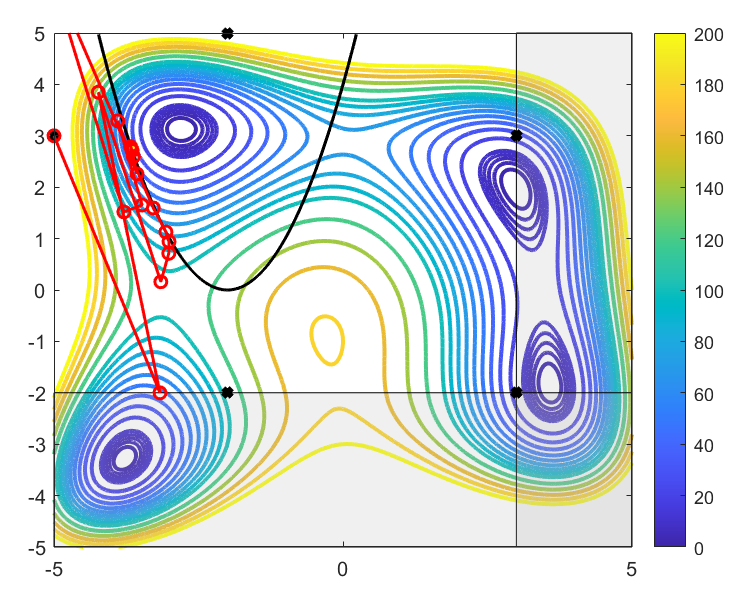
\includegraphics[scale=0.4]{figures/SQP_BFGS_LINE_A.PNG}
%\caption{fig1}
}
\quad
\subfigure[$B(-2,-2)$]{
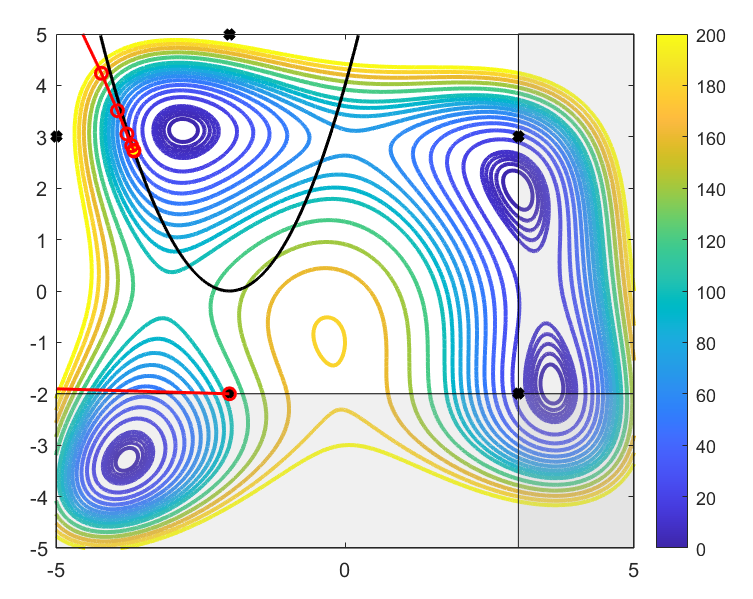
\includegraphics[scale=0.4]{figures/SQP_BFGS_LINE_B.PNG}
}
\quad
\subfigure[$C(3,3)$]{
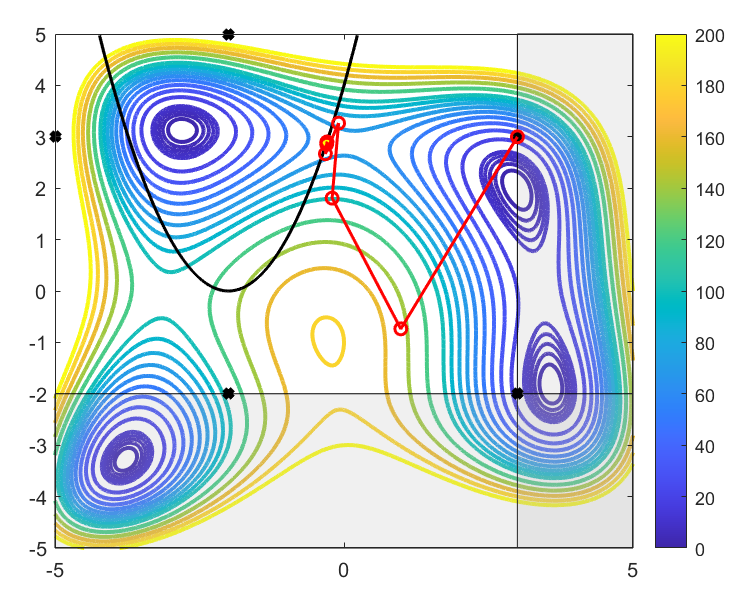
\includegraphics[scale=0.4]{figures/SQP_BFGS_LINE_C.PNG}
}
\quad
\subfigure[$D(-2,5)$]{
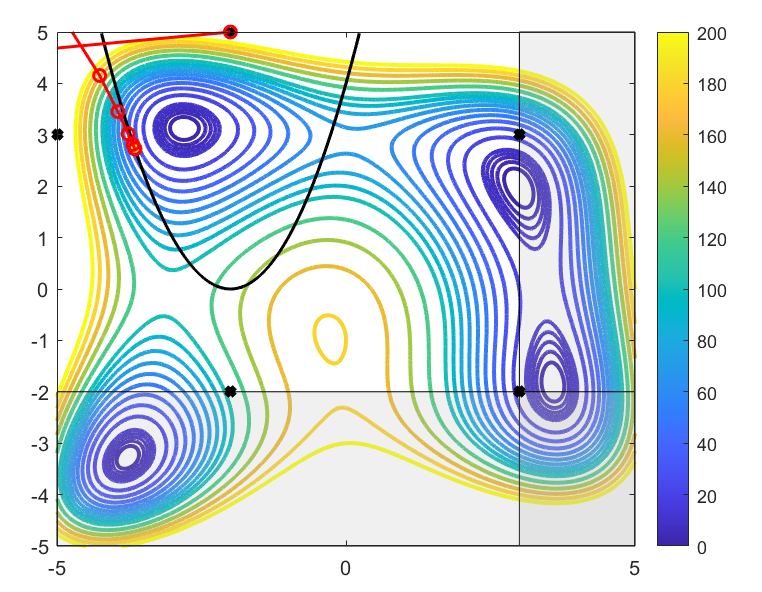
\includegraphics[scale=0.4]{figures/SQP_BFGS_LINE_D.PNG}
}
\quad
\subfigure[$E(3,-2)$]{
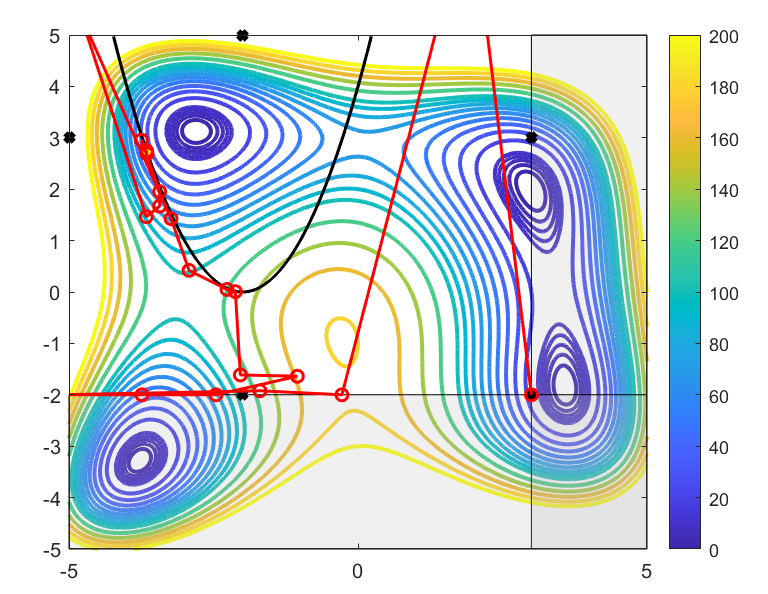
\includegraphics[scale=0.4]{figures/SQP_BFGS_LINE_E.PNG}
}
\caption{ Iterative trajectory in contour}
\end{figure}
%%%%%%%%%%%%%%%%%%%%%%%%%%%%%%%%%%%%%%%%%%%%%%%%%%%%%%%
The iteration of table is showed here separately
%%%%%%%%%%%%%%%%%%%%%%%%%%%%%%%%%%%%%%%%%%%%%%%%%%%%%%
\begin{table}[H]
\centering
\setlength{\abovecaptionskip}{0cm} 
\setlength{\belowcaptionskip}{-0.5cm}
\scriptsize
\begin{tabular}{|c|c|c|c|c|c|c|c|c|c|c|}
\hline
$x_0=A(-5,3)$&0&1&2&3&4&5&6&7&8&9\\
\hline
$x_1$&-5.0 & -3.17 & -4.23 & -3.15 & -3.01 & -3.01 & -3.06 & -3.28 & -5.09 & -3.79 \\
\hline
$x_2$&3.0 & -2.0 & 3.85 & 0.16 & 0.713 & 0.941 & 1.13 & 1.6 & 6.28 & 1.52 
\\
\hline
\end{tabular}
\begin{tabular}{|c|c|c|c|c|c|c|c|c|c|}
\hline
$x_0=A(-5,3)$&10&11&12&13&14&15&16&17&18\\
\hline
$x_1$ &3.48 & -3.9 & -3.56 & -3.63 & -3.67 & -3.65 & -3.65 & -3.65 & -3.65\\
\hline
$x_2$ & 1.65 & 3.29 & 2.26 & 2.59 & 2.79 & 2.71 & 2.74 & 2.74 & 2.74
\\
\hline

\end{tabular}
\caption{$x_0=A(-5,3)$}
\end{table}

%%%%%%%%%%%%%%%%%%%%%%%%%%%%%%%%%%%%%%%%%%%%%%%%%%%%%%%%%
\begin{table}[H]
\centering
\setlength{\abovecaptionskip}{0cm} 
\setlength{\belowcaptionskip}{-0.5cm}
\scriptsize
\begin{tabular}{|c|c|c|c|c|c|c|c|c|c|c|}
\hline
$x_0=B(-2,-2)$&0&1&2&3&4&5&6&7&8&9\\
\hline
$x_1$&-2.0 & -64.0 & -40.8 & -27.2 & -17.8 & -12.3 & -8.79 & -6.69 & -5.42 & -4.67  \\
\hline
$x_2$&-2.0 & 0 & -1.49 & 70.8 & 16.4 & 15.7 & 11.5 & 8.89 & 6.79 & 5.31   
\\
\hline
\end{tabular}

\begin{tabular}{|c|c|c|c|c|c|c|c|c|}
\hline
$x_0=B(-2,-2)$&10&11&12&13&14&15&16&17\\
\hline
$x_1$&-4.21 & -3.94 & -3.77 & -3.69 & -3.65 & -3.65 & -3.65 & -3.65  \\
\hline
$x_2$&4.24 & 3.51 & 3.06 & 2.83 & 2.72 & 2.74 & 2.74 & 2.74
\\
\hline
\end{tabular}

\caption{$x_0=B(-2,-2)$}
\end{table}
%%%%%%%%%%%%%%%%%%%%%%%%%%%%%%%%%%%%%%%%%%%%%%%%%%%%%%%%%%%%%
\begin{table}[H]
\centering
\setlength{\abovecaptionskip}{0cm} 
\setlength{\belowcaptionskip}{-0.5cm}
\scriptsize
\begin{tabular}{|c|c|c|c|c|c|c|c|c|c|c|}
\hline
$x_0=C(3,3)$&0&1&2&3&4&5&6&7&8&9\\
\hline
$x_1$&3.0 & 0.983 & -0.206 & -0.0934 & -0.322 & -0.299 & -0.294 & -0.299 & -0.298 & -0.298 \\
\hline
$x_2$&3.0 & -0.736 & 1.81 & 3.27 & 2.67 & 2.86 & 2.9 & 2.89 & 2.9 & 2.9
\\
\hline
\end{tabular}

\caption{$x_0=C(3,3)$}
\end{table}
%%%%%%%%%%%%%%%%%%%%%%%%%%%%%%%%%%%%%%%%%%%%%%%%%%%%%%%%%%%%%%%
\begin{table}[H]
\centering
\setlength{\abovecaptionskip}{0cm} 
\setlength{\belowcaptionskip}{-0.5cm}
\scriptsize
\begin{tabular}{|c|c|c|c|c|c|c|c|c|c|c|}
\hline
$x_0=D(-2,5)$&0&1&2&3&4&5&6&7&8&9\\
\hline
$x_1$&-2.0 & -50.0 & -32.1 & -21.4 & -14.1 & -9.83 & -7.22 & -5.68 & -4.79 & -4.26  \\
\hline
$x_2$&5.0 & 0 & -1.49 & 36.5 & 7.73 & 7.46 & 6.86 & 6.04 & 5.1 & 4.15
\\
\hline
\end{tabular}
\begin{tabular}{|c|c|c|c|c|c|c|c|c|c|c|c|}
\hline
$x_0=D(-2,5)$&10&11&12&13&14&15&16\\
\hline
$x_1$ &-3.95 & -3.77 & -3.69 & -3.65 & -3.65 & -3.65 & -3.65\\
\hline
$x_2$&  3.45 & 3.02 & 2.81 & 2.72 & 2.74 & 2.74 & 2.74
\\
\hline

\end{tabular}
\caption{$x_0=D(-2,5)$}
\end{table}
%%%%%%%%%%%%%%%%%%%%%%%%%%%%%%%%%%%%%%%%%%%%%%%%%%%%%%%%%%%
\begin{table}[H]
\centering
\setlength{\abovecaptionskip}{0cm} 
\setlength{\belowcaptionskip}{-0.5cm}
\scriptsize
\begin{tabular}{|c|c|c|c|c|c|c|c|c|c|c|}
\hline
$x_0=E(3,-2)$&0&1&2&3&4&5&6&7&8&9\\
\hline
$x_1$&3.0 & 1.95 & -0.278 & -1.7 & -5.15 & -3.74 & -2.46 & -1.05 & -2.04 & -2.12  \\
\hline
$x_2$&-2.0 & 7.67 & -2.0 & -1.92 & -2.0 & -2.0 & -2.0 & -1.64 & -1.61 & 0.00732 
\\
\hline
\end{tabular}
\begin{tabular}{|c|c|c|c|c|c|c|c|c|c|c|}
\hline
$x_0=E(3,-2)$&10&11&12&13&14&15&16&17&18&19\\
\hline
$x_1$ &-2.27 & -2.92 & -3.24 & -4.81 & -3.66 & -3.43 & -3.43 & -3.75 & -3.65 & -3.66\\
\hline
$x_2$&   0.05 & 0.42 & 1.43 & 5.4 & 1.46 & 1.67 & 1.95 & 2.96 & 2.69 & 2.75
\\
\hline

\end{tabular}
\begin{tabular}{|c|c|c|c|}
\hline
$x_0=E(3,-2)$&20&21&22\\
\hline
$x_1$ &-3.65 & -3.65 & -3.65\\
\hline
$x_2$&   2.74 & 2.74 & 2.74
\\
\hline

\end{tabular}
\caption{$x_0=E(3,-2)$}
\end{table}

It can be seen that starting points $A$, $B$,$D$, and $E$ have reached the correct minimum points, but starting points $C$ reached a sub-minimum point. The success rate of SQP with BFGS and line search is higher than the previous algorithm(without line search), and the number of iterations is also reduced compared to the previous algorithm\\

First analyze from the contours with starting points $B$ and $D$. These two points in the previous algorithm(without line search) can only find the sub-minimum point because the step size of the sub-problem solution is too large, but after adding the line search algorithm, it is found that the amplitude of the step size did not change too much, so the minimum point was successfully found. Similarly, the points $C$ and $E$ mentioned earlier accidentally crossed the area where the maximum point was found because of the large step size, but after adding the line search, although the step size of $E$ point is still too large , the step size of point $C$ is obviously suppressed, and the sub-minimum point is found in the right half of the equality constraint curve.

%%%%%%%%%%%%%%%%%%%%%%%%%%%%%%%%%%%%%%%%%%
%%%%%%%%%%%%%%%%%%%%%%%%%%%%%%%%%%%%%%%%%%%
%%%%%%%%%%%%%%%%%%%%%%%%%%%%%%%%%%%%%%%%%%
%%%%%%%%%%%%%%%%%%%%%%%%%%%%%%%%%%%%%%%%%%%
%%%%%%%%%%%%%%%%%%%%%%%%%%%%%%%%%%%%%%%%%%
%%%%%%%%%%%%%%%%%%%%%%%%%%%%%%%%%%%%%%%%%%%
\newpage
\subsection{\bfseries Trust Region based SQP algorithm}
\begin{shaded}
{Question:Explain, discuss, and implement a Trust Region based SQP algorithm for this
problem. Make a table with the iteration sequence. Make a table with
relevant statistics (function calls etc). Plot the iteration sequence in a contour
plot. Discuss the results}
\end{shaded}
In the trust region method, the parameter $\Delta _k$ is used to control the quality of the steps as the size of the trust region. The simplest way to formulate a trust-region SQP method is to add a trust-region constraint to subproblem

$$\begin{aligned}
\min _{\Delta x \in \mathbb{R}^{n}} \qquad & \frac{1}{2} \Delta x^{\prime}\left[\nabla_{x x}^{2} L\left(x_{k}, \mu_{k},\lambda_{k}\right)\right] \Delta x+\left[\nabla_{x} L\left(x_{k}, \mu_{k},\lambda_{k}\right)\right]^{\prime} \Delta x \\
\text {s.t.} \qquad & \nabla g\left(x_{k}\right)^{\prime} \Delta x=-g\left(x_{k}\right)\\
& \nabla h\left(x_{k}\right)^{\prime} \Delta x\ge -h\left(x_{k}\right)\\
& \left\| p\right \|\le \Delta_k
\end{aligned}\eqno{(5.37)}$$

However, even if the constraints are compatible, this problem may not always have a solution because of the trust-region constraint. Here, the S$l1$QP is introduced. In this approach the linearized constraints are moved into the objective of the quadratic program, in the form of an $l1$ penalty term, to obtain the following subproblem by introducing
slack variables $v4$, $w$, $t$:
\begin{align*}
\min _{p, v, w, t} \quad &f_{k}+\nabla f_{k}^{T} p+\frac{1}{2} p^{T} \nabla_{x x}^{2} \mathcal{L}_{k} p+\mu \sum_{i \in \mathcal{E}}\left(v_{i}+w_{i}\right)+\mu \sum_{i \in \mathcal{I}} t_{i}\tag{5.38}\\
s.t.\quad & \nabla g_{i}\left(x_{k}\right)^{T} p+g_{i}\left(x_{k}\right)=v_{i}-w_{i}\\
&\nabla h_{i}\left(x_{k}\right)^{T} p+h_{i}\left(x_{k}\right) \geq-t_{i}\\
&v, w, t \geq 0\\
&\|p\|_{\infty} \leq \Delta_{k}
\end{align*}

This formulation is simply a linearization of the elastic-mode formulation with the
addition of a trust-region constraint.
The constraints of this problem are always consistent. Since the trust region has been
defined using the $l \infty$ norm, is a smooth quadratic program that can be solved
by means of a quadratic programming algorithm.\\
\newpage
After computing the step $p_k$, the ratio $\rho_k$ is determined via

$$\rho_{k}=\frac{\operatorname{ared}_{k}}{\operatorname{pred}_{k}}=\frac{\phi_{1}\left(x_{k}, \mu\right)-\phi_{1}\left(x_{k}+p_{k}, \mu\right)}{q_{\mu}(0)-q_{\mu}\left(p_{k}\right)}\eqno{(5.39)}$$

Use the merit function $\phi1$ and defining $q_{\mu}$ by

$$q_{\mu}(p)=f_{k}+\nabla f_{k}^{\prime} p+\frac{\sigma}{2} p^{\prime} \nabla_{x x}^{2} \mathcal{L}_{k} p+\mu m_{k}(p)\eqno{(5.40)}$$
Where
$$m(p)=\left\|g(x_k)+\nabla g(x_k)p_k\right\|_1+\left\|h(x_k)+\nabla h(x_k)p_k\right\|_1\eqno{(5.41)}$$

Then the most important step is to choose a suitable $\mu$ at each iterates, because the $\mu$ plays an important role in the efficiency of this method. The step $p_k$ directly depends on the value of $\mu$. Values of $\mu$ that are too small can lead the algorithm away from the solution, while excessively large values can result in slow progress. A penalty update and step computation algorithm is stated here


\begin{algorithm}[H]
	\caption{ Penalty Update}
	\begin{algorithmic}[1]
	    \STATE Given $x_k,\mu_{k-1}>0$,$\delta_k>0$,and parameters $\eta_1,\eta_2 \in (0,1)$\\
		\IF{($m_k(p(\mu_{k-1}))$)}\\
		\STATE Set $\mu_k=\mu_{k-1}$\\
        \ELSE\\
		\STATE Compute the $p_{\infty}$\\
		\IF{($m_k(p_{\infty})$)}\\
		\STATE Find $\mu{k}>\mu_{k-1}$ such that $m_k(p(\mu_{k}))=0$\\
		\ELSE\\
		\STATE Find $\mu{k}>\mu_{k-1}$ such that$m_k(0)-m_k(p(\mu_{k}))\ge \eta_1\left[m_k(0)-m_k(p(\infty)\right]$
		\ENDIF\\
		\ENDIF\\
		\STATE increas $\mu_k$ if necessary to satisfy$q_{\mu_k}(0)-q_{\mu_k}(p(\mu_k))\ge \eta_2\mu_k\left[m_k(0)-m_k(p(\mu_{k}))\right]$
    \end{algorithmic}
\end{algorithm}

The step is accepted or rejected
according to standard trust-region rules, as implemented in pseudo-code\\
\newpage
{\setmainfont{Times New Roman}\bfseries Pseudo-code}
\begin{algorithm}[H]
	\caption{ Trust Region based SQP algorithm}
	\begin{algorithmic}[1]
	    \STATE Given a starting point($x_0,\mu_0,\lambda_0$), set $k=0$. Choose $\eta \in (0,1), \tau \in (0,0.5)$\\
		\STATE Evaluate $f_0,\nabla f_0,g_0,\nabla g_0,h_0,\nabla h_0$\\
		\STATE Choose an initial $n \times n$ symmetric positive definite Hessian approximation $B_0$, always an Identity matrix\\
        \WHILE {(not converged)}\\
		\STATE Compute the $p_k$($\Delta x_k$),$\mu_{k+1}$ and $\lambda_{k+1}$by solving the sub-quadratic-problem\\
		\STATE Set $p_{\lambda}=\lambda_{k+1}-\lambda_{k}$\\
		\STATE Compute $\mu$ with the penalty update algorithm stated above\\
		\STATE Compute $\rho_k=ared_k/pred_k$\\
		\IF{($\rho_k>\eta$)}\\
		\STATE Set $x_{k+1}=x_k+p_k$\\
		\STATE Choose $\Delta_{K+1}$ to satisfy $\Delta_{K+1}\ge \Delta_{K}$\\
		\ELSE\\
		\STATE Set $x_{k+1}=x_k$\\
		\STATE Choose $\Delta_{K+1}$ to satisfy $\Delta_{K+1}\le \gamma \|p_k\|$\\
		\ENDIF\\
		\STATE Compute $\nabla_{x}L\left(x_{k}, \mu_{k+1},\lambda_{k+1}\right)=\nabla f(x_k)-\nabla g(x_k)\mu_{k+1}-\nabla h(x_k)\lambda_{k+1}$\\
		\STATE Evaluate $f_{k+1},\nabla f_{k+1},g_{k+1},\nabla g_{k+1},h_{k+1},\nabla h_{k+1}$\\
		\STATE Compute $\nabla_{x}L\left(x_{k+1}, \mu_{k+1},\lambda_{k+1}\right)=\nabla f(x_{k+1})-\nabla g(x_{k+1})\mu_{k+1}-\nabla h(x_{k+1})\lambda_{k+1}$\\
		\STATE Compute the $s_k$ and $y_k$\\
		\STATE Update the Hessian matrix by the modified BFGS procedure\\
		\STATE $k=k+1$\\
		\ENDWHILE
    \end{algorithmic}
\end{algorithm}



Next the specific Matlab code of implementation is showed. The function "Hg_f" which calculate the gradients and hessian of object-function and itself, the "Hg_ceq" which calculate the gradients and hessian of equality constraints and itself, the "Hg_ciq" which calculate the gradients and hessian of equality constraints and itself, the "Qpsolver_Sqp" which solve the sub-problem of SQP algorithm are stated in appendix \ref{6.5.4}, \ref{6.5.5}, \ref{6.5.6} and \ref{6.5.7}. Only the main program is showed here

{\setmainfont{Courier New Bold} \scriptsize         
\begin{lstlisting}
function [x,output]=Sqp_Bfgs_trust(x0,lam_eq0,lam_ineq0)
% Sqp_Bfgs_trust   SQP algorithm with damped BFGS and line search
%
%          min  f(x)
%           x
%          s.t. ceq(x)=0  (Lagrange multiplier lam_eq)    
%               ciq(x)>=0  (Lagrange multiplier lam_ineq)  
% Syntax: [x,output]=Sqp_Bfgs_trust(x0,lam_eq0,lam_ineq0)
%         output.fval: minimum value
%         output.dL: convergence of delta_L
%         output.ceq: convergence of ceq
%         output.Xarray=Xarray: Iteration trajectory  
epsilon=1e-6;
ro=0.99;
gamma=0.9;
eta=0.2;
eta2=0.2;
eta3=0.5;
deltak=0.9;

deltaAarray=[];
deltaAarray=[deltaAarray deltak];
mu=30;
Xarray=[];
normdLarray=[];
normceqarray=[];
Xarray=[Xarray x0];

nx=size(x0,1);
Bk=eye(nx);

[f,df,~]=Hg_f(x0);
[ceq,dceq,~]=Hg_ceq(x0);
[ciq,dciq,~]=Hg_ciq(x0);

xk=x0;
lam_eqk=lam_eq0;
lam_ineqk=lam_ineq0;
iteration=0;
iteration_max=80;
iter_line_max=30;
while(iteration<iteration_max)
    %Solve the subproblem(QP)
    %Linearization of the elastic-mode formulation
    
    H_L1=[Bk zeros(2,2) zeros(2,2);zeros(4,6)];
    df_L1=[df;mu;mu;mu;mu];
    dciq_L1=[dciq' [1 0 0 0;0 1 0 0];zeros(4,2) eye(4);...
       [1 0 0 0 0 0];[0 1 0 0 0 0];[-1 0 0 0 0 0];[0 -1 0 0 0 0]];
    ciq_L1=[-ciq;zeros(4,1);-deltak;-deltak;-deltak;-deltak];
    dceq_L1=[dceq' 0 0 -1 1];
    ceq_L1=[-ceq];
    [p_all,~,~,~,lamk] = quadprog(H_L1,df_L1,-dciq_L1,-ciq_L1,dceq_L1,ceq_L1);
    p=p_all(1:2);
    lamineq=lamk.ineqlin(1:2); 
    
    lameq=lamk.eqlin;
    lam_eqk_hat=-lameq;
    lam_ineqk_hat=-lamineq;
    lam_eqk=lam_eqk_hat;
    lam_ineqk=lam_ineqk_hat;
    
    %evaluate the gradient
    [f_new,~,~]=Hg_f(xk+p);
    [ceq_new,~,~]=Hg_ceq(xk+p);
    [ciq_new,~,~]=Hg_ciq(xk+p);
    
   
    mp_eq=norm((ceq+dceq'*p),1);
    mp_ineq=norm(min(0,(ciq+dciq'*p)),1);
    mp_k=mp_eq+mp_ineq;
    %Penalty update and step computation
    if mp_k==0
        mu=mu;
    else
        p_norm=norm(p,"Inf");
        mp_eq_inf=norm((ceq+dceq'*p),1);
        mp_ineq_inf=norm(min(0,(ciq+dciq'*p)),1);
        mp_k_inf=mp_eq+mp_ineq;
        if mp_k_inf==0
            mu=mu*(1+eta2);
        else
        if norm(ceq,1)+norm(min(0,ciq),1)-mp_k>=eta3*(norm(ceq,1)+norm(min(0,ciq),1)-mp_k_inf)
            mu=mu;
        else
            mu=mu*(1+eta2);
        end
        end
    end
    %calculate the ratio
    qmu_p=f+df'*p+0.5*p'*Bk*p+mu*mp_eq+mu*mp_ineq;
    qmu_zero=f+mu*norm((ceq),1)+mu*norm(min(0,ciq),1);
    predk=qmu_zero-qmu_p;
   
    phi1=f+mu*norm(ceq,1)+mu*norm(min(0,ciq),1);
    phi1_new=f_new+mu*norm(ceq_new,1)+mu*norm(min(0,ciq_new),1);
    aredk=phi1-phi1_new;
    rok=aredk/predk;
    %judge the step is accepted or rejected
    if rok>eta
        xk=xk+p;
        deltak=1.5*deltak;
    else
        deltak=gamma*norm(p,"Inf");
    end
   
    %Calculate dL(k) with x(k) and lameq(k+1),lamineq(k+1)
    Lk=df-dceq.*lam_eqk-dciq*lam_ineqk;
    %Re-evaluate
    [f,df,~]=Hg_f(xk);
    [ceq,dceq,~]=Hg_ceq(xk);
    [ciq,dciq,~]=Hg_ciq(xk);
    %Calculate L(k+1) with x(k+1) and lam(k+1)
    Lk2=df-dceq.*lam_eqk-dciq*lam_ineqk;
    %Damped BFGS update
    pk=p;
    qk=Lk2-Lk;
    
    judge=(pk'*qk>=0.2*pk'*(Bk*pk));
    thetak=judge.*1+(~judge).*((0.8*pk'*(Bk*pk))/(pk'*(Bk*pk)-pk'*qk));
    rk=thetak*qk+(1-thetak)*(Bk*pk);
    Bk=Bk-((Bk*pk)*(pk'*Bk))/(pk'*(Bk*pk))+(rk*rk')/(pk'*rk);
    %Check teh convergence
    if ((norm(Lk2,"inf")<epsilon)&&(norm(ceq,"inf")<epsilon)&&(max(abs(ciq)) + epsilon >= 0)...
       &&(min(lam_ineqk) + epsilon >= 0))
        break;
    end
    iteration=iteration+1;
    Xarray=[Xarray xk];
    normdLarray=[normdLarray norm(Lk2,"inf")];
    normceqarray=[normceqarray norm(ceq,"inf")];
    deltaAarray=[deltaAarray deltak];
end
[fval,~,~]=Hg_f(xk);
x=xk;
output.fval=fval;
output.xarray=Xarray;
output.dL=normdLarray;
output.ceq=normceqarray;
output.iteration=iteration;
output.delta=deltaAarray;
end
\end{lstlisting}}
%%%%%%%%%%%%%%%%%%%%%%%%%%%%%%%%%%%%%%%%%%%%%%%%%%%%%%%%
The algorithm will be tested with the same initial
points as in the section 5.5. Please see the test code in Appendix \ref{6.5.10}. Iterative trajectory of starting points $A$, $B$, $C$, $D$ and $E$ in the contour is showed 
\begin{figure}[H]
\centering
\subfigure[$A(-5,3)$]{
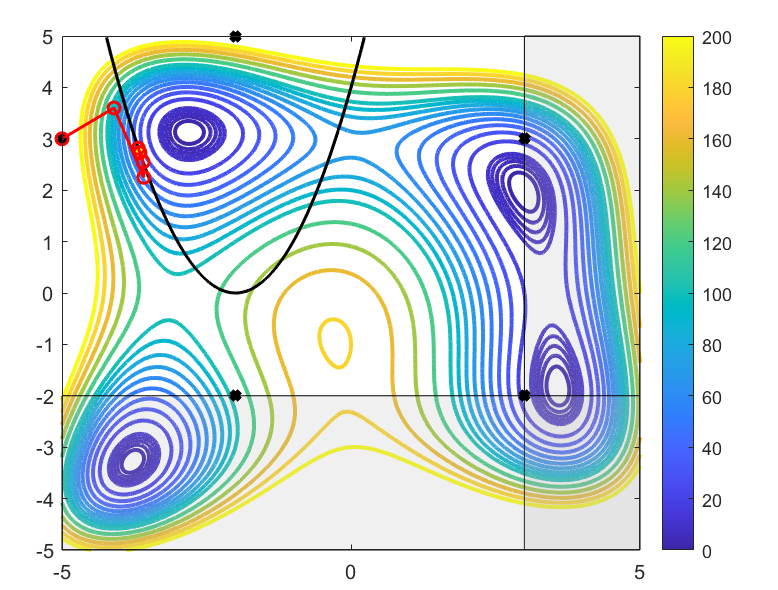
\includegraphics[scale=0.4]{figures/SQP_BFGS_TRUST_A.PNG}
%\caption{fig1}
}
\quad
\subfigure[$B(-2,-2)$]{
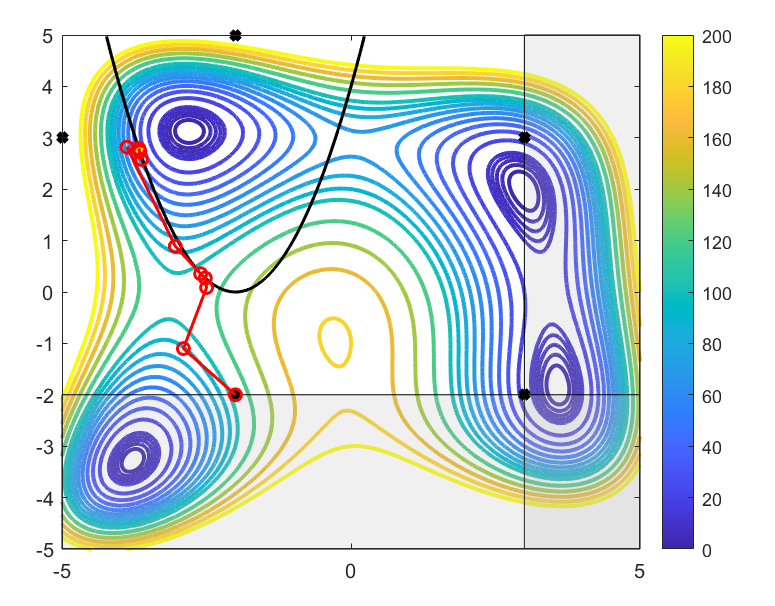
\includegraphics[scale=0.4]{figures/SQP_BFGS_TRUST_B.PNG}
}
\quad
\subfigure[$C(3,3)$]{
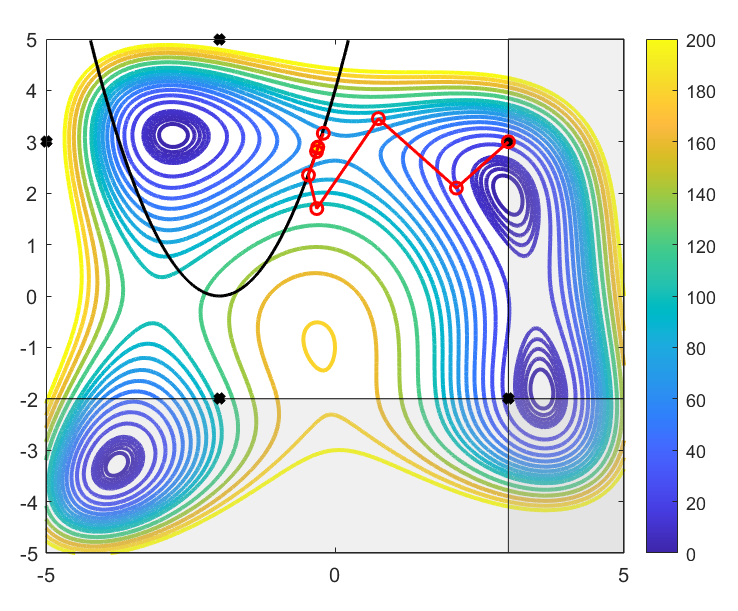
\includegraphics[scale=0.4]{figures/SQP_BFGS_TRUST_C.PNG}
}
\quad
\subfigure[$D(-2,5)$]{
\includegraphics[scale=0.4]{figures/SQP_BFGS_TRUST_D.PNG}
}
\quad
\subfigure[$E(3,-2)$]{
\includegraphics[scale=0.4]{figures/SQP_BFGS_TRUST_E.PNG}
}
\caption{ Iterative trajectory in contour}
\end{figure}

%%%%%%%%%%%%%%%%%%%%%%%%%%%%%%%%%%%%%%%%%%%%%%%%%%%%%%%
The iteration of table is showed here separately
%%%%%%%%%%%%%%%%%%%%%%%%%%%%%%%%%%%%%%%%%%%%%%%%%%%%%%
\begin{table}[H]
\centering
\setlength{\abovecaptionskip}{0cm} 
\setlength{\belowcaptionskip}{-0.5cm} 
\scriptsize
\begin{tabular}{|c|c|c|c|c|c|c|c|c|}
\hline
$x_0=A(-5,3)$&0&1&2&3&4&5&6&7\\
\hline
$x_1$&-5.0 & -4.1 & -3.59 & -3.6 & -3.68 & -3.65 & -3.65 & -3.65\\
\hline
$x_2$&3.0 & 3.6 & 2.25 & 2.55 & 2.82 & 2.73 & 2.74 & 2.74
\\
\hline
\end{tabular}
\caption{$x_0=A(-5,3)$}
\end{table}

%%%%%%%%%%%%%%%%%%%%%%%%%%%%%%%%%%%%%%%%%%%%%%%%%%%%%%%%%
\begin{table}[H]
\centering
\setlength{\abovecaptionskip}{0cm} 
\setlength{\belowcaptionskip}{-0.5cm} 
\scriptsize
\begin{tabular}{|c|c|c|c|c|c|c|c|c|c|c|}
\hline
$x_0=B(-2,-2)$&0&1&2&3&4&5&6&7&8&9\\
\hline
$x_1$&-2.0 & -2.9 & -2.5 & -2.52 & -2.6 & -3.04 & -3.04 & -3.04 & -3.04 & -3.04 \\
\hline
$x_2$&-2.0 & -1.1 & 0.0876 & 0.271 & 0.355 & 0.888 & 0.888 & 0.888 & 0.888 & 0.888 
\\
\hline
\end{tabular}

\begin{tabular}{|c|c|c|c|c|c|c|c|c|c|c|}
\hline
$x_0=B(-2,-2)$&10&11&12&13&14&15&16&17&18&19\\
\hline
$x_1$&-3.04 & -3.04 & -3.04 & -3.04 & -3.04 & -3.04 & -3.04 & -3.04 & -3.88 & -3.63  \\
\hline
$x_2$&0.888 & 0.888 & 0.888 & 0.888 & 0.888 & 0.888 & 0.888 & 0.888 & 2.82 & 2.58
\\
\hline
\end{tabular}
\begin{tabular}{|c|c|c|c|c|}
\hline
$x_0=B(-2,-2)$&20&21&22&23\\
\hline
$x_1$ &-3.67 & -3.65 & -3.65 & -3.65\\
\hline
$x_2$&  2.79 & 2.73 & 2.74 & 2.74\\
\hline

\end{tabular}
\caption{$x_0=B(-2,-2)$}
\end{table}
%%%%%%%%%%%%%%%%%%%%%%%%%%%%%%%%%%%%%%%%%%%%%%%%%%%%%%%%%%%%%
\begin{table}[H]
\centering
\setlength{\abovecaptionskip}{0cm} 
\setlength{\belowcaptionskip}{-0.5cm} 
\scriptsize
\begin{tabular}{|c|c|c|c|c|c|c|c|c|c|c|}
\hline
$x_0=C(3,3)$&0&1&2&3&4&5&6&7&8&9\\
\hline
$x_1$&3.0 & 2.1 & 0.75 & -0.316 & -0.46 & -0.202 & -0.32 & -0.301 & -0.298 & -0.298 \\
\hline
$x_2$&3.0 & 2.1 & 3.45 & 1.7 & 2.35 & 3.17 & 2.81 & 2.89 & 2.9 & 2.9
\\
\hline
\end{tabular}

\caption{$x_0=C(3,3)$}
\end{table}
%%%%%%%%%%%%%%%%%%%%%%%%%%%%%%%%%%%%%%%%%%%%%%%%%%%%%%%%%%%%%%%
\begin{table}[H]
\centering
\setlength{\abovecaptionskip}{0cm} 
\setlength{\belowcaptionskip}{-0.5cm} 
\scriptsize
\begin{tabular}{|c|c|c|c|c|c|c|c|c|c|c|}
\hline
$x_0=D(-2,5)$&0&1&2&3&4&5&6&7&8&9\\
\hline
$x_1$&-2.0 & -2.9 & -2.9 & -2.9 & -3.99 & -3.99 & -3.99 & -3.42 & -3.61 & -3.61  \\
\hline
$x_2$&5.0 & 4.1 & 4.1 & 4.1 & 3.01 & 3.01 & 3.01 & 1.68 & 2.54 & 2.54
\\
\hline
\end{tabular}
\begin{tabular}{|c|c|c|c|c|c|}
\hline
$x_0=D(-2,5)$&10&11&12&13&14\\
\hline
$x_1$ &-3.72 & -3.65 & -3.65 & -3.65 & -3.65\\
\hline
$x_2$& 2.94 & 2.72 & 2.74 & 2.74 & 2.74
\\
\hline

\end{tabular}
\caption{$x_0=D(-2,5)$}
\end{table}
%%%%%%%%%%%%%%%%%%%%%%%%%%%%%%%%%%%%%%%%%%%%%%%%%%%%%%%%%%%
\begin{table}[H]
\centering
\setlength{\abovecaptionskip}{0cm} 
\setlength{\belowcaptionskip}{-0.5cm} 
\scriptsize
\begin{tabular}{|c|c|c|c|c|c|c|c|c|}
\hline
$x_0=E(3,-2)$&0&1&2&3&4&5&6&7\\
\hline
$x_1$&3.0 & 2.1 & 0.75 & -0.211 & -0.31 & -0.296 & -0.298 & -0.298 \\
\hline
$x_2$&-2.0 & -1.1 & 0.25 & 2.27 & 2.85 & 2.9 & 2.9 & 2.9
\\
\hline
\end{tabular}

\caption{$x_0=E(3,-2)$}
\end{table}
It can be seen that starting points $A$, $B$, and $D$ have reached the correct minimum points, but starting points $C$ and $E$ reached a sub-minimum point, which has the same result as one solved by fmincon.\\
From the contours of $A$, $B$, and $D$ starting points that successfully reach the minimum point, the step size of each iteration is adjusted appropriately, and the minimum point can be reached with a small number of iterations. The effect is obviously better than the line search method. At the same time, from the contours of $C$ and $E$ starting points that reach the sub-minimum point. Because the step size is appropriately limited, there is no large jump in iteration process of $C$ and $E$ as before, skipping the area where the maximum value is, and accidentally reaching the left half part of the equality constraint curve and finds the minimum point, but iterates normally to the right half part of the equality constraint curve and finds the sub-minimum point.
Through the comparison of these three methods(SQP with BFGS, SQP with BFGS and line search, SQP based on trust region), it is found that the trust region based method adjusts the step size more accurately, can be more stable, and obtain better results.
%%%%%%%%%%%%%%%%%%%%%%%%%%%%%%%%%%%%%%%%%%
%%%%%%%%%%%%%%%%%%%%%%%%%%%%%%%%%%%%%%%%%%%
%%%%%%%%%%%%%%%%%%%%%%%%%%%%%%%%%%%%%%%%%%
%%%%%%%%%%%%%%%%%%%%%%%%%%%%%%%%%%%%%%%%%%%
%%%%%%%%%%%%%%%%%%%%%%%%%%%%%%%%%%%%%%%%%%
%%%%%%%%%%%%%%%%%%%%%%%%%%%%%%%%%%%%%%%%%%%
\subsection{\bfseries Primal-Dual Interior Point Algorithms for NLP}
\begin{shaded}
{Question:Explain, discuss, and implement an interior-point algorithm for this problem.
Make a table with the iteration sequence. Make a table with relevant statistics
(function calls etc). Plot the iteration sequence in a contour plot. Discuss the
results}
\end{shaded}
First, the nonlinear problem can be written as follows by introducing the slack variables

$$\begin{aligned}
\min _{x,s} \qquad & f(x) \\
\text {s.t.} \qquad & g(x)=0\\
& h(x)-s=0\\
& s\ge 0
\end{aligned}\eqno{(5.42)}$$

Then the KKT condition can be expressed as
\begin{align*}
&\nabla_{x} L(x, y, z)=\nabla f(x)-\nabla g(x) y-\nabla h(x) z=0 \tag{5.43}\\
&g(x)=0 \tag{5.44}\\
&h(x)-s=0 \tag{5.45}\\
&S z=0 \tag{5.46}\\
&s \geq 0 \quad z \geq 0 \tag{5.47}
\end{align*}
In the interior point algorithms a perturbed KKT system is solved

$$S z=0 \Leftrightarrow Sz-\tau e=0\eqno{(5.48)}$$

Then apply the Newton's method and obtain the primal-dual system

$$\left[\begin{array}{cccc}
\nabla_{x x}^{2} L(x, y, z) & 0 & -\nabla g(x) & -\nabla h(x) \\
0 & Z & 0 & S \\
\nabla g(x)^{\prime} & 0 & 0 & 0 \\
\nabla h(x)^{\prime} & -I & 0 & 0
\end{array}\right]\left[\begin{array}{c}
p_{x} \\
p_{s} \\
p_{y} \\
p_{z}
\end{array}\right]=-\left[\begin{array}{c}
\nabla_{x} L(x, y, z) \\
S z-\tau e \\
g(x) \\
h(x)-s
\end{array}\right]\eqno{(5.49)}$$
which is equivalent to the symmetric system

$$\left[\begin{array}{cccc}
\nabla_{x x}^{2} L(x, y, z) & 0 & \nabla g(x) & \nabla h(x) \\
0 & \Sigma & 0 & -I \\
\nabla g(x)^{\prime} & 0 & 0 & 0 \\
\nabla h(x)^{\prime} & -I & 0 & 0
\end{array}\right]\left[\begin{array}{c}
p_{x} \\
p_{s} \\
-p_{y} \\
-p_{z}
\end{array}\right]=-\left[\begin{array}{c}
\nabla_{x} L(x, y, z) \\
z-\tau S^{-1} e \\
g(x) \\
h(x)-s
\end{array}\right]\eqno{(5.50)}$$
Where
$$\Sigma =S^{-1}Z\eqno{(5.51)}$$
Compute the step length 

$$\begin{array}{l}
\alpha_{s}=\max \left\{\alpha \in(0,1]: s+\alpha p_{s} \geq \eta s\right\}\eqno{(5.52)} \\
\alpha_{z}=\max \left\{\alpha \in(0,1]: z+\alpha p_{z} \geq \eta z\right\}\eqno{(5.53)}
\end{array}$$

Then update the new iterate
\begin{align*}
    x_{k+1}&=x_k+ \alpha_sp_x \tag{5.54}\\
    s_{k+1}&=s_k+ \alpha_sp_s\tag{5.55}\\
    y_{k+1}&=y_k+ \alpha_zp_y\tag{5.56}\\
    z_{k+1}&=z_k+ \alpha_zp_z\tag{5.57}
\end{align*}
About the check of convergence, the error measure is defined

$$E(x, s, y, z ; \tau)=\|F(x, s, y, z ; \tau)\|\eqno{(5.58)}$$
Where
$$\begin{aligned}
&F(x, s, y, z ; \tau)=\left[\begin{array}{c}
\nabla_{x} L(x, y, z) \\
S z-\tau e \\
g(x) \\
h(x)-s
\end{array}\right]=\left[\begin{array}{l}
0 \\
0 \\
0 \\
0
\end{array}\right]=0\\
&(s, z) \geq 0
\end{aligned}\eqno{(5.59)}$$
\newpage
{\setmainfont{Times New Roman}\bfseries Pseudo-code}
\begin{algorithm}[H]
	\caption{Primal-Dual Interior Point Algorithms for NLP}
	\begin{algorithmic}[1]
	    \STATE Choose $x_0$,$s_0>0$. Compute initial values for $y_0$, $z_0$\\
		\STATE Select $\tau_0$, $\eta=0.005$,$\rho \in (0,1)$, $k=0$\\
		\WHILE {($E(x_k,s_k,y_k,z_k,0)>\epsilon$)}\\
		\WHILE {($E(x_k,s_k,y_k,z_k,\tau_k)>\tau_k$)}\\
		\STATE Solve the primal-dual system to obtain the search direction $p_x$, $p_s$, $p_y$, $p_z$.\\
		\STATE Compute the step length $\alpha_s^{max}$, $\alpha_z^{max}$\\
		\STATE Update the iterate $x_{k+1}$, $s_{k+1}$, $y_{k+1}$, $z_{k+1}$, $k=k+1$\\
		\ENDWHILE\\
		\STATE Choose $\tau_k \in (0,\rho  \tau_k)$\\
		\ENDWHILE
    \end{algorithmic}
\end{algorithm}
Next the specific Matlab code of implementation is showed. The function "Hg_f" which calculate the gradients and hessian of object-function and itself, the "Hg_ceq" which calculate the gradients and hessian of equality constraints and itself, the "Hg_ciq" which calculate the gradients and hessian of equality constraints and itself are stated in Appendix \ref{6.5.4}, \ref{6.5.5} and \ref{6.5.6}. Only the main program is showed here

{\setmainfont{Courier New Bold} \scriptsize         
\begin{lstlisting}
function [x,output]=ipNLP(x0,y0,z0,s0)
% ipNLP   Primal-Dual Interior Point Algorithms for NLP
%
%          min  f(x)
%           x
%          s.t. ceq(x)=0  (Lagrange multiplier y)    
%               ciq(x)-s=0  (Lagrange multiplier z)
%               s>=0
%          rdL=df-dceq*y-dciq*z;
%          rsz=S*z-tau*e;
%          rceq=ceq;
%          rciq=ciq-s;
% Syntax: [x,output]=ipNLP(x0,y0,z0,s0)
%         output.fval: minimum value
%         output.Xarray=Xarray: Iteration trajectory  
epsilon=1.0e-5;
tau0=0.8;
eta=0.005;
ro=0.5;
Xarray=[];
Xarray=[Xarray x0];

nx=size(x0,1);
neq=size(y0,1);
niq=size(z0,1);
e=ones(niq,1);
%evaluate the gradient and hessian
[f,df,d2f]=Hg_f(x0);
[ceq,dceq,d2ceq]=Hg_ceq(x0);
[ciq,dciq,d2ciq]=Hg_ciq(x0);

xk=x0;
yk=y0;
Z0=diag(z0);
S0=diag(s0);
Zk=Z0;
Sk=S0;
tauk=tau0;
iteration=0;
iteration_out=0;
iteration_max=700;
iteration_max_out=700;
while(iteration_out<iteration_max_out)
    %convergence judge
    
    rdL=df-dceq*yk-dciq*diag(Zk);
    rsz=Sk*diag(Zk)-0*e;
    rceq=ceq;
    rciq=ciq-diag(Sk);
    Error=max([norm(rdL,1),norm(rsz,1),norm(rceq,1),norm(rciq,1)]);
    if Error<epsilon
        break;
    end
    while(iteration<iteration_max)
        %solve the subproblem
        [f,df,d2f]=Hg_f(xk);
        [ceq,dceq,d2ceq]=Hg_ceq(xk);
        [ciq,dciq,d2ciq]=Hg_ciq(xk);
        sk=diag(Sk);
        zk=diag(Zk);
        sumeq=0;
        sumiq=0;
        for i=1:length(yk)
            sumeq=sumeq+yk(i)*d2ceq(:,:,i);
        end
        for i=1:length(zk)
            sumiq=sumiq+zk(i)*d2ciq(:,:,i);
        end
        ddL=d2f-sumeq-sumiq;
        sumk=inv(Sk)*Zk;
        KKT_A=[ddL,zeros(nx,niq),dceq,dciq;zeros(niq,nx),sumk,zeros(niq,neq),-eye(niq);...
           dceq',zeros(neq,niq),zeros(neq,neq),zeros(neq,niq);dciq',-eye(niq),zeros(niq,neq),...
           zeros(niq,niq)];
        rdL=df-dceq*yk-dciq*zk;
        rsz=zk-tauk.*inv(Sk)*e;
        rceq=ceq;
        rciq=ciq-sk;
        KKT_b=-[rdL;rsz;rceq;rciq];
        [L,D,p]=ldl(KKT_A,'vector');
        p_all=zeros(size(KKT_b,1),1);
        p_all(p)=L'\(D\(L\KKT_b(p)));
        px=p_all(1:nx);
        ps=p_all(nx+1:nx+niq);
        py=-p_all(nx+niq+1:nx+niq+neq);
        pz=-p_all(nx+niq+neq+1:end);
        %compute the step length
        alpha_tmp_s=(eta.*sk-sk)./ps;
        alpha_s=min([1;alpha_tmp_s(ps<0)]);
        alpha_tmp_z=(eta.*zk-zk)./pz;
        alpha_z=min([1;alpha_tmp_z(pz<0)]);
        %Update x_k+1, y_k+1, s_k+1, z_k+1
        xk=xk+alpha_s*px;
        sk=sk+alpha_s*ps;
        yk=yk+alpha_z*py;
        zk=zk+alpha_z*pz;
        Sk=diag(sk);
        Zk=diag(zk);
        iteration=iteration+1;
        Xarray=[Xarray xk];
        %convergence judge
        rdL=df-dceq*yk-dciq*zk;
        rsz=Sk*zk-tauk.*e;
        rceq=ceq;
        rciq=ciq-diag(Sk);
        Error=max([norm(rdL,1),norm(rsz,1),norm(rceq,1),norm(rciq,1)]);
        if Error<tauk
            break;
        end
    end
    tauk=ro*tauk;
    iteration_out=iteration_out+1;
end
x=xk;
[fval,~,~]=Hg_f(xk);
output.xarray=Xarray;
output.iteration=iteration;
output.fval=fval;
end
\end{lstlisting}}
The algorithm will be tested with the same initial
points as in the section 5.5. Please see the test code in Appendix \ref{6.5.11}. Iterative trajectory of starting points $A$, $B$, $C$, $D$ and $E$ in the contour is showed 
\begin{figure}[H]
\centering
\subfigure[$A(-5,3)$]{
\includegraphics[scale=0.4]{figures/IP_NLP_A.PNG}
%\caption{fig1}
}
\quad
\subfigure[$B(-2,-2)$]{
\includegraphics[scale=0.4]{figures/IP_NLP_B.PNG}
}
\quad
\subfigure[$C(3,3)$]{
\includegraphics[scale=0.4]{figures/IP_NLP_C.PNG}
}
\quad
\subfigure[$D(-2,5)$]{
\includegraphics[scale=0.4]{figures/IP_NLP_D.PNG}
}
\quad
\subfigure[$E(3,-2)$]{
\includegraphics[scale=0.4]{figures/IP_NLP_E.PNG}
}
\caption{ Iterative trajectory in contour}
\end{figure}

%%%%%%%%%%%%%%%%%%%%%%%%%%%%%%%%%%%%%%%%%%%%%%%%%%%%%%%
The iteration of table is showed here separately
%%%%%%%%%%%%%%%%%%%%%%%%%%%%%%%%%%%%%%%%%%%%%%%%%%%%%%
\begin{table}[H]
\centering
\setlength{\abovecaptionskip}{0cm} 
\setlength{\belowcaptionskip}{-0.5cm} 
\scriptsize
\begin{tabular}{|c|c|c|c|c|c|c|c|c|c|}
\hline
$x_0=A(-5,3)$&0&1&2&3&4&5&6&7\\
\hline
$x_1$&-5.0 & -3.99 & -3.7 & -3.66 & -3.66 & -3.66 & -3.65 & -3.65 \\
\hline
$x_2$&3.0 & 2.91 & 2.81 & 2.75 & 2.74 & 2.74 & 2.74 & 2.74
\\
\hline
\end{tabular}
\caption{$x_0=A(-5,3)$}
\end{table}

%%%%%%%%%%%%%%%%%%%%%%%%%%%%%%%%%%%%%%%%%%%%%%%%%%%%%%%%%

%%%%%%%%%%%%%%%%%%%%%%%%%%%%%%%%%%%%%%%%%%%%%%%%%%%%%%%%%
\begin{table}[H]
\centering
\setlength{\abovecaptionskip}{0cm} 
\setlength{\belowcaptionskip}{-0.5cm} 
\scriptsize
\begin{tabular}{|c|c|c|c|c|c|c|c|c|c|c|}
\hline
$x_0=B(-2,-2)$&0&1&2&3&4&5&6&7&8&9\\
\hline
$x_1$&-2.0 & -28.8 & -23.2 & -12.6 & -11.1 & -9.7 & -8.33 & -7.18 & -6.24 & -5.48 \\
\hline
$x_2$&-2.0 & 0 & -1.99 & 1.53 & -1.98 & 57.2 & 38.2 & 25.5 & 17.1 & 11.5
\\
\hline
\end{tabular}

\begin{tabular}{|c|c|c|c|c|c|c|c|c|c|c|}
\hline
$x_0=B(-2,-2)$&10&11&12&13&14&15&16&17&18&19\\
\hline
$x_1$&-4.87 & -4.39 & -4.03 & -3.79 & -3.68 & -3.66 & -3.66 & -3.66 & -3.65 & -3.65   \\
\hline
$x_2$&7.86 & 5.47 & 3.99 & 3.15 & 2.81 & 2.74 & 2.74 & 2.74 & 2.74 & 2.74  
\\
\hline
\end{tabular}
\caption{$x_0=B(-2,-2)$}
\end{table}
%%%%%%%%%%%%%%%%%%%%%%%%%%%%%%%%%%%%%%%%%%%%%%%%%%%%%%%%%%%%%
\begin{table}[H]
\centering
\setlength{\abovecaptionskip}{0cm} 
\setlength{\belowcaptionskip}{-0.5cm} 
\scriptsize
\begin{tabular}{|c|c|c|c|c|c|c|c|c|}
\hline
$x_0=C(3,3)$&0&1&2&3&4&5&6&7\\
\hline
$x_1$&3.0 & 0.803 & -0.0717 & -0.282 & -0.298 & -0.298 & -0.298 & -0.298 \\
\hline
$x_2$&3.0 & 3.03 & 2.95 & 2.91 & 2.9 & 2.9 & 2.9 & 2.9  
\\
\hline
\end{tabular}

\caption{$x_0=C(3,3)$}
\end{table}
%%%%%%%%%%%%%%%%%%%%%%%%%%%%%%%%%%%%%%%%%%%%%%%%%%%%%%%%%%%%%%%
\begin{table}[H]
\centering
\setlength{\abovecaptionskip}{0cm} 
\setlength{\belowcaptionskip}{-0.5cm} 
\scriptsize
\begin{tabular}{|c|c|c|c|c|c|c|c|c|}
\hline
$x_0=D(-2,5)$&0&1&2&3&4&5&6&7\\
\hline
$x_1$&-2.0 & -1.48 & -1.47 & -1.42 & -1.43 & -1.43 & -1.42 & -1.42   \\
\hline
$x_2$&5.0 & 0 & 0.285 & 0.33 & 0.33 & 0.33 & 0.331 & 0.331
\\
\hline
\end{tabular}
\caption{$x_0=D(-2,5)$}
\end{table}
%%%%%%%%%%%%%%%%%%%%%%%%%%%%%%%%%%%%%%%%%%%%%%%%%%%%%%%%%%%
\begin{table}[H]
\centering
\setlength{\abovecaptionskip}{0cm} 
\setlength{\belowcaptionskip}{-0.5cm} 
\scriptsize
\begin{tabular}{|c|c|c|c|c|c|c|c|c|c|c|}
\hline
$x_0=E(3,-2)$&0&1&2&3&4&5&6&7&8&9\\
\hline
$x_1$&3.0 & 0.415 & -0.997 & -1.34 & -1.45 & -1.43 & -1.43 & -1.43 & -1.42 & -1.42 \\
\hline
$x_2$&-2.0 & -0.855 & -0.987 & 0.326 & 0.289 & 0.33 & 0.33 & 0.33 & 0.331 & 0.331 
\\
\hline
\end{tabular}

\caption{$x_0=E(3,-2)$}
\end{table}
It can be seen that starting points $A$ and $B$ have reached the correct minimum points, but starting points $C$ reached a sub-minimum point, and the starting points $D$ and $E$ reached a sub-minimum.\\
First of all, based on the analysis in the previous chapter, it is inferred that the starting points $A$, $B$, and $C$ are the correct iteration trajectories, where the starting point $B$ has many iterations and oscillations, which is related to the choice of step size.
Observing the iterative trajectory of the starting point $D$, it is also speculated that $D$ also jumped directly to a region far away from the correct minimum point because of the too long step size, and instead found the sub-minimum point that meets the convergence condition,
The point E is to approximate the equality constraint curve , and directly passes through the area where the maximum value is located, and also finds the sub-minimum point that meets the convergence condition.

%%%%%%%%%%%%%%%%%%%%%%%%%%%%%%%%%%%%%%%%%%
%%%%%%%%%%%%%%%%%%%%%%%%%%%%%%%%%%%%%%%%%%%
%%%%%%%%%%%%%%%%%%%%%%%%%%%%%%%%%%%%%%%%%%
%%%%%%%%%%%%%%%%%%%%%%%%%%%%%%%%%%%%%%%%%%%
%%%%%%%%%%%%%%%%%%%%%%%%%%%%%%%%%%%%%%%%%%
%%%%%%%%%%%%%%%%%%%%%%%%%%%%%%%%%%%%%%%%%%%
\newpage
\subsection{\bfseries Comparison of algorithms}
\begin{shaded}
{Question:Discuss the different algorithms, the performance of the different algorithms, and
your implementations. In general provide any comments and discussion that
demonstrates that you have an excellent overview of nonlinear programing}
\end{shaded}
First, three methods in the SQP algorithm will be discussed. First the SQP algorithm with damped BFGS and SQP algorithm with damped BFGS and line search are compared. Regardless of whether the step size is limited or not based on line search, these two methods use Newton's method, which is to solve the quadratic programming problem of Taylor quadratic expansion at the current point to determine a search direction, but the method based on line search Finding an optimal step size along this direction makes the objective function drop the most at this step size. It can be seen from the test results of the two algorithms that the method based on line search has fewer iterations, and it can be seen from the iterative curve that the iteration point is easy to produce a larger number based on the Newton method without restricting the step size Jump and oscillate and increase the number of iterations.  Both methods are easy to fall into the local minimum. Compared with this, the SQP method based on the trust region has better performance.\\

In each iteration of the trust region method, first determine a radius of the trust region, and then calculate the minimum value of the second-order approximation of the objective function within the radius. If the minimum value makes the objective function achieve a sufficient decline, then enter the next iteration and expand the radius of the trust region. If the minimum value cannot make the objective function obtain a sufficient decline, it means that the current order of trust region The approximation is not reliable enough, it is necessary to reduce the radius of the trust region and recalculate the minimum value. In the usual nonlinear problem, taking the test problem selected this time as an example, it can be seen that the objective function has four local minimum and one local maximum. If the second-order approximation of the objective function at the current point is close to a local minimum point and is very different from the global minimum point, the line-based search method will find the local minimum point, but the trust region method is reasonably selected In the case of the radius of the trust region, the step size can be controlled more reasonably until the global minimum point is found to achieve a better result. As can be seen from the test results of the algorithm, the iterative curve path based on the trust region is shorter, and there are no unnecessary oscillations and jumps, and the number of iterations is also less. \\

On the formulation of the quadratic subproblem, the IQP approach is used in SQP algorithm with damped BFGS and SQP algorithm with damped BFGS and line search. Because the test question designed here has only two variables, it cannot reflect the high expense of solving the general quadratic subproblem when the nonlinear problem is large. In contrast,in the trust region-based method, the S$l1$QP approach which is an example of EQP method is used to move the linearized constraints into the objective of the quadratic program in the form of an $l1$ penalty term.  The EQP method can have less expense than IQP method in the large-scale cases. Then the S$l1$QP approach further not only can overcome the possible inconsistency among the linearized constraints, but it also ensures that the trust region constraint can always be satisfied.\\

The interior point method implemented in this report is the basic interior point method. A step selection method is used such as line search and trust domain implemented in SQP, so the test results obtained are slightly worse than expected.
Both the continuous method and the obstacle method are applied. The KKT condition of the original problem is converted to the prime-dual system, and gradually change the barrier parameter $\mu$ to search for a central path to gradually optimize the original problem. Among them, the continuous method defines and finds the iterative direction of the prime-dual system. The barrier method guarantees the convergence of the global iteration by moving the barrier parameter to 0. For the update of the barrier parameter, the Fiacco-McCormick approach is used to make the barrier parameter limited to 0. Although this method can achieve good results in most cases, in some cases the choice of the initial point, the initial barrier parameter value, and the scaling of the problem can make problem vulnerable. In order to increase the robustness for all situations, the Adaptive strategies \cite{NoceWrig06} is recommended.\\

Compare SQP with the interior point method. First, SQP is applicable when the number of constraints and the number of variables is very close, because expense can be saved in the formulation and solution of sub-problem in each step. In contrast, the sub-problem solved by each iteration of the interior point method is the same, so it is possible to save iteration expense by optimizing the formulation of the sub-problem. Moreover, because the interior point method iterates within the feasible region, it does not consider all constraints in each iteration, but removes constraints that are not related to the optimal solution, saving iteration costs. Finally, the SQP shows better robustness on badly scaled problems than the nonlinear interior point method.


\newpage
\newpage
% \\section{References}

\bibliographystyle{unsrt}
\bibliography{bibtex/ref}

\newpage
\section{ \bfseries Appendix}
%%%%%%%%%%%%%%%%%%%%%%%%%%%%%%%%%%%%%%%%%%%%%%%%%%%%%%%%%%%%%%%%%%%%%%%%%%%%%%%%%%%%%%%%%%%%%%%%%%%%%%%%%%%%%%%%%%%%%%%%%%%%%%%%%%%%%%%%%%%%%%%%
\subsection{\bfseries Question 1 }

\subsubsection{\bfseries EqualityQPSolver }
\label{6.1.1}
{\setmainfont{Courier New Bold} \scriptsize         
\begin{lstlisting}
function [x,lambda]=EqualityQPSolver(H,g,A,b,solver)
%EqualityQPSolver  Equality constrained convex QP

%Syntax: [x,lambda]=EqualityQPSolver(H,g,A,b,solver)
%solver is a flag used to switch between the different factorizations
%solver : 'LUdense'----->LUfactorization (dense)
%         'LUsparse'---->LUfactorization (sparse)
%         'LDLdense'---->LDL-factorization (dense)
%         'LDLsparse'--->LDL-factorization (sparse)
%         'RangeSpace'-->Range-Space factorization
%         'NullSpace'--->Null-Space factorization
switch solver
    case 'LUdense'
        [x,lambda]=EqualityQPSolverLUdense(H,g,A,b);
    case 'LUsparse'
        [x,lambda]=EqualityQPSolverLUsparse(H,g,A,b);
    case 'LDLdense'
        [x,lambda]=EqualityQPSolverLDLdense(H,g,A,b);
    case 'LDLsparse'
        [x,lambda]=EqualityQPSolverLDLsparse(H,g,A,b);
    case 'RangeSpace'
        [x,lambda]=EqualityQPSolverRangeSpace(H,g,A,b);
    case 'NullSpace'
        [x,lambda]=EqualityQPSolverNullSpace(H,g,A,b);
    otherwise 
        x=[];
        lambda=[];
end
\end{lstlisting}}
%%%%%%%%%%%%%%%%%%%%%%%%%%%%%%%%%%%%%%%%%%%%%%%%%%%%%%%%%%%%%%%%%%%%%%%%%%%%%%%%%%%%%%%%%%%%%%%%%%%%%%%%%%%%%%%%%%%%%%%%%%%%%%%%%%%%%%%%%%%%%%%%%%%%%%%%%%%%%%%%%%%%%%%%%%%%%%%%%%%%%%%%%%%%%%%%%%%%%%%%%%%%%%%%%%%%%%%%
\subsubsection{\bfseries u2HgAb }
\label{6.1.2}
{\setmainfont{Courier New Bold} \scriptsize         
\begin{lstlisting}
function [H,g,A,b]=u2HgAb(n,u_mean,d0)
%u2HgAb  Generate the H,g,A,b of test problem

%Syntax: [H,g,A,b]=u2HgAb(n,u_mean,d0)
%n: The number of variables
%u_mean,d0: The changed constant in test problem
H=eye(n+1);
g=-2*u_mean*ones(n+1,1);
b=zeros(n, 1);
b(1,1)=-d0;
A=[zeros(1,n-1);eye(n-1)];
A=[A zeros(n,1)]-eye(n);
A=A';
A=[A; zeros(1, n)];
A(n,1)=1;
A(n+1,n)=-1;
end
\end{lstlisting}}
%%%%%%%%%%%%%%%%%%%%%%%%%%%%%%%%%%%%%%%%%%%%%%%%%%%%%%%%%%%%%%%%%%%%%%%%%%%%%%%%%%%%%%%%%%%%%%%%%%%%%%%%%%%%%%%%%%%%%%
\subsubsection{\bfseries Test code of question1 }
\label{6.1.3}
{\setmainfont{Courier New Bold} \scriptsize         
\begin{lstlisting}
%test code of Question1 
%Only the test of LU-dense is showed here.
%Change the solver from 'LUdense' to 'LUsparse', 'LDLdense'
%'LDLsparse', 'RangeSpace', 'NullSpace'
clear all
k=0
record_LUd=zeros(991,1);
record_LDLd=zeros(991,1);
record_LDLs=zeros(991,1);
record_rs=zeros(991,1);
record_ns=zeros(991,1);
for n=10:1000
    [H, g, A, b] = u2HgAb(n, 0.2,1);
    while(1)
    tic;
    [x,lambda]=EqualityQPSolver(H,g,A,b,'LUdense');
    elapsedTime = toc;
    if n==10
        break;
    end
    if elapsedTime<1.5*record_LUd(n-10)
        break;
    end
    end
    record_LUd(n-9)=elapsedTime;
    k=k+1
end
\end{lstlisting}}
%%%%%%%%%%%%%%%%%%%%%%%%%%%%%%%%%%%%%%%%%%%%%%%%%%%%%%%%%%%%%%%%%%%%%%%%%%%%%%%%%%%%%%%%%%%%%%%%%%%%%%%%%%%%%%%%%%%%%%%%%%%%%%%%%%%%%%%%%%%%%%%%%%%%%%%%%%%%%%%%%%%%%%%%%%%%%%%%%%%%%%%%%%%%%%%%%%%%%%%%%%%%%%%%%%%%%%%%
\subsection{\bfseries Question 2 }

\subsubsection{bfseries Test code of Prime-IP for QP with equality and inequality}
\label{6.2.1}
{\setmainfont{Courier New Bold} \scriptsize         
\begin{lstlisting}
%Primal-dual interior-point algorithm for QP 
%test code for problem1 with equality and inequality constraints
H=[2,0;0,2];
g=[-2;-5];
Ae=[1 -1];
be=[1];
Ai=[1 0;-1 0;0 1;0 -1];
bi=[-1;-2;-1;-2];
x0=[0 0]';
y0=1;
z0=ones(4,1);
s0=ones(4,1);
[x,output]=PD_ipQP(H,g,Ae',be,Ai',bi,x0,y0,z0,s0)
\end{lstlisting}}
%%%%%%%%%%%%%%%%%%%%%%%%%%%%%%%%%%%%%%%%%%%%%%%%%%%%%%%%%%%%%%%%%%%%%%%%%%%%%%%%%%%%%%%%%%%%%%%%%%%%%%%%%%%%%%%%%%%%%%%%%%%%%%%%%%%%%%%%%%%%%%%%%%%%%%%%%%%%%%%%%%%%%%%%%%%%%%%%%%%%%%%%%%%%%%%%%%%%%%%%%%%%%%%%%%%%%%%%
\subsubsection{\bfseries Test code of Prime-IP for QP with only inequality}
\label{6.2.2}
{\setmainfont{Courier New Bold} \scriptsize         
\begin{lstlisting}
%Primal-dual interior-point algorithm for QP 
%test code for problem1 with only inequality constraints
H=[2,0;0,2];
g=[-2;-5];
Ae=[];
be=[];
Ai=[1 0;-1 0;0 1;0 -1];
bi=[-1;-2;-1;-2];
x0=[0 0]';
y0=0;
z0=ones(4,1);
s0=ones(4,1);
[x,output]=PD_ipQP(H,g,Ae',be,Ai',bi,x0,y0,z0,s0)
\end{lstlisting}}
%%%%%%%%%%%%%%%%%%%%%%%%%%%%%%%%%%%%%%%%%%%%%%%%%%%%%%%%%%%%%%%%%%%%%%%%%%%%%%%%%%%%%%%%%%%%%%%%%%%%%%%%%%%%%%%%%%%%%%%%%%%%%%%%%%%%%%%%%%%%%%%%%%%%%%%%%%%%%%%%%%%%%%%%%%%%%%%%%%%%%%%%%%%%%%%%%%%%%%%%%%%%%%%%%%%%%%%%

\subsubsection{\bfseries As_sub }
\label{6.2.3}
{\setmainfont{Courier New Bold} \scriptsize         
\begin{lstlisting}
function [p,lambda]=As_sub(H,g,Ae,be)
%EQP solver for the primal active set method
ginvH=pinv(H);
[n,m]=size(Ae);
%For singular matrices caused by equality constraints
if(n>0)
    rb=Ae*ginvH*g+be;
    lambda=pinv(Ae*ginvH*Ae')*rb;
    p=ginvH*(Ae'*lambda-g);
else
    p=-ginvH*g;
    lambda=0;
end
\end{lstlisting}}
%%%%%%%%%%%%%%%%%%%%%%%%%%%%%%%%%%%%%%%%%%%%%%%%%%%%%%%%%%%%%%%%%%%%%%%%%%%%%%%%%%%%%%%%%%%%%%%%%%%%%%%%%%%%%%%%%%%%%%%%%%%%%%%%%%%%%%%%%%%%%%%%%%%%%%%%%%%%%%%%%%%%%%%%%%%%%%%%%%%%%%%%%%%%%%%%%%%%%%%%%%%%%%%%%%%%%%%%
\subsubsection{\bfseries Test code of Prime Active set for QP with equality and inequality}
\label{6.2.4}
{\setmainfont{Courier New Bold} \scriptsize         
\begin{lstlisting}
%Primal Active-Set Algorithm for QP 
%test code for problem1 with equality and inequality constraints
H=[2,0;0,2];
g=[-2;-5];
Ae=[1 -1];
be=[1];
Ai=[1 0;-1 0;0 1;0 -1];
bi=[-1;-2;-1;-2];
x0=[1;0];
[x,lamk,exitflag,output]=Pri_AsQp(H,g,Ae,be,Ai,bi,x0)
\end{lstlisting}}
%%%%%%%%%%%%%%%%%%%%%%%%%%%%%%%%%%%%%%%%%%%%%%%%%%%%%%%%%%%%%%%%%%%%%%%%%%%%%%%%%%%%%%%%%%%%%%%%%%%%%%%%%%%%%%%%%%%%%%%%%%%%%%%%%%%%%%%%%%%%%%%%%%%%%%%%%%%%%%%%%%%%%%%%%%%%%%%%%%%%%%%%%%%%%%%%%%%%%%%%%%%%%%%%%%%%%%%%
\subsubsection{\bfseries Test code of Prime Active set for QP with only inequality}
\label{6.2.5}
{\setmainfont{Courier New Bold} \scriptsize         
\begin{lstlisting}
%Primal Active-Set Algorithm for QP 
%test code for problem1 with only inequality constraints
H=[2,0;0,2];
g=[-2;-5];
Ae=[];
be=[];
Ai=[1 0;-1 0;0 1;0 -1];
bi=[-1;-2;-1;-2];
x0=[-1;0];
[x,lamk,exitflag,output]=Pri_AsQp(H,g,Ae,be,Ai,bi,x0)
\end{lstlisting}}
%%%%%%%%%%%%%%%%%%%%%%%%%%%%%%%%%%%%%%%%%%%%%%%%%%%%%%%%%%%%%%%%%%%%%%%%%%%%%%%%%%%%%%%%%%%%%%%%%%%%%%%%%%%%%%%%%%%%%%%%%%%%%%%%%%%%%%%%%%%%%%%%%%%%%%%%%%%%%%%%%%%%%%%%%%%%%%%%%%%%%%%%%%%%%%%%%%%%%%%%%%%%%%%%%%%%%%%%
\subsubsection{\bfseries Test code of three methods for QP problem with n changed}
\label{6.2.6}
{\setmainfont{Courier New Bold} \scriptsize         
\begin{lstlisting}
%test code of three methods with variable number changed from 10 to 200
%Primal-dual interior-point, Primal Active-Set and quadprog 
niparray=[];
nasarray=[];
nquadarray=[];
itip=[];
itas=[];
itquad=[];
for i=10:10:200
    %intialization of test problem
    n=i;
    m=0.5*n;
    X=rand(n);
    H=X'*X+eye(n);
    A=randn(m,n);
    x=zeros(n,1);
    x(1:m,1)=abs(rand(m,1))*10;
    lambda=zeros(n,1);
    lambda(m+1:n,1)=abs(rand(n-m,1))*10;
    mu=rand(m,1);
    g=A'*mu+lambda-H*x;
    b=A*x;
    Ae=A;
    be=b;
    Ai=[eye(n);-eye(n)];
    bi=[zeros(n,1);-10*ones(n,1)];
    %calculate the starting feasible point using linprog
    options = optimoptions('linprog','Algorithm','dual-simplex');
    x0_as = linprog(g,-Ai,-bi,Ae,be,[],[],options);
    y0=ones(m,1);
    z0=ones(2*n,1);
    s0=ones(2*n,1);
    %Primal-dual interior-point
    [x_out,output1]=PD_ipQP(H,g,Ae',be,Ai',bi,x0_as,y0,z0,s0);
    nip=norm(x_out-x,2);
    %Primal Active-Set Algorithm
    [x_as,lamk,exitflag,output2]=Pri_AsQp(H,g,Ae,be,Ai,bi,x0_as);
    nas=norm(x_as-x,2);
    %quadprog 
    options2 = optimoptions('quadprog','Display','iter','Algorithm',...
        "interior-point-convex");
    [x_quad,fval,exitflag,output3,lambda] = ...
        quadprog(H,g,-Ai,-bi,Ae,be,[],[],x0_as,options2);
    nquad=norm(x_quad-x,2);
    niparray=[niparray nip];
    nasarray=[nasarray nas];
    nquadarray=[nquadarray nquad];
    itip=[itip output1.iteration];
    itas=[itas output2.iter];
    itquad=[itquad output3.iterations];
end
\end{lstlisting}}
%%%%%%%%%%%%%%%%%%%%%%%%%%%%%%%%%%%%%%%%%%%%%%%%%%%%%%%%%%%%%%%%%%%%%%%%%%%%%%%%%%%%%%%%%%%%%%%%%%%%%%%%%%%%%%%%%%%%%%%%%%%%%%%%%%%%%%%%%%%%%%%%%%%%%%%%%%%%%%%%%%%%%%%%%%%%%%%%%%%%%%%%%%%%%%%%%%%%%%%%%%%%%%%%%%%%%%%%
\subsubsection{\bfseries Test code of Markowitz’ portfolio optimization problem as QP}
\label{6.2.7}
{\setmainfont{Courier New Bold} \scriptsize         
\begin{lstlisting}
%Markowitz’ portfolio optimization problem as QP
clear all
H=[2.30 0.93 0.62 0.74 -0.23
    0.93 1.40 0.22 0.56 0.26
    0.62 0.22 1.80 0.78 -0.27
    0.74 0.56 0.78 3.40 -0.56
    -0.23 0.26 -0.27 -0.56 2.60];
miu=[15.10;12.50;14.70;9.02;17.68];
Ae=[-miu';1 1 1 1 1];
be=[-10;1];
Ai=-eye(5);
bi=zeros(5,1);
g=zeros(5,1);
%calculate the starting feasible point 
options1 = optimoptions('linprog','Algorithm','dual-simplex');
x0_as = linprog([],Ai,bi,Ae,be,[],[],options1)

%quadprog
options2 = optimoptions('quadprog','Display','iter','Algorithm',...
   "interior-point-convex");
[x_q,fval,exitflag,output,lambda] = ...
   quadprog(H,[],Ai,bi,Ae,be,zeros(5,1),[],x0_as,options2)
r_q1=miu'*x_q %return
var_q1=2*fval %risk
%Primal-dual interior-point
y0=ones(2,1);
z0=ones(5,1);
s0=ones(5,1);
[x_out,output1]=PD_ipQP(H,g,Ae',be,-Ai',-bi,x0_as,y0,z0,s0)
r_q2=miu'*x_out %return
var_q2=2*output1.fval %risk
%Primal Active-Set
[x_as,lamk,exitflag,output2]=Pri_AsQp(H,g,Ae,be,-Ai,-bi,x0_as)
r_q3=miu'*x_out %return
var_q3=2*output2.fval %risk

\end{lstlisting}}
%%%%%%%%%%%%%%%%%%%%%%%%%%%%%%%%%%%%%%%%%%%%%%%%%%%%%%%%%%%%%%%%%%%%%%%%%%%%%%%%%%%%%%%%%%%%%%%%%%%%%%%%%%%
\subsection{\bfseries Question 3 }

\subsubsection{\bfseries Test code of portfolio with exactly return 10}
\label{6.3.1}
{\setmainfont{Courier New Bold} \scriptsize         
\begin{lstlisting}
clear all;
H=[2.30 0.93 0.62 0.74 -0.23
    0.93 1.40 0.22 0.56 0.26
    0.62 0.22 1.80 0.78 -0.27
    0.74 0.56 0.78 3.40 -0.56
    -0.23 0.26 -0.27 -0.56 2.60];
miu=[15.10;12.50;14.70;9.02;17.68];
Ae=[-miu';1 1 1 1 1];
be=[-10;1];
Ai=-eye(5);
bi=zeros(5,1);
options = optimoptions('quadprog','Display','iter','Algorithm',...
   "interior-point-convex");
[x,fval,exitflag,output,lambda] = ...
   quadprog(H,[],Ai,bi,Ae,be,zeros(5,1),[],[],options)
r=miu'*x
var_s=2*fval
\end{lstlisting}}
%%%%%%%%%%%%%%%%%%%%%%%%%%%%%%%%%%%%%%%%%%%%%%%%%%%%%%%%%%%%%%%%%%%%%%%%%%%%%%%%%%%%%%%%%%%%%%%%%%%%%%%%%%%%%%%%%%%%%%%%%%%%%%%%%%%%%%%%%%%%%%%%%%%%%%%%%%%%%%%%%%%%%%%%%%%%%%%%%%%%%%%%%%%%%%%%%%%%%%%%%%%%%%%%%%%%%%%%
\subsubsection{\bfseries Test code of portfolio with maximal return over 10}
\label{6.3.2}
{\setmainfont{Courier New Bold} \scriptsize         
\begin{lstlisting}
%To achieve the highest possible return with the minimum variance
H=[2.30 0.93 0.62 0.74 -0.23
    0.93 1.40 0.22 0.56 0.26
    0.62 0.22 1.80 0.78 -0.27
    0.74 0.56 0.78 3.40 -0.56
    -0.23 0.26 -0.27 -0.56 2.60];
miu=[15.10;12.50;14.70;9.02;17.68];
Ae=[1 1 1 1 1];
be=[1];
Ai=[-miu';-eye(5)];
bi=[-10;zeros(5,1)];
options = optimoptions('quadprog','Display','iter','Algorithm',...
   "interior-point-convex");
[x,fval,exitflag,output,lambda] = ...
   quadprog(H,[],Ai,bi,Ae,be,zeros(5,1),[],[],options)
r=miu'*x
var_s=2*fval
\end{lstlisting}}
%%%%%%%%%%%%%%%%%%%%%%%%%%%%%%%%%%%%%%%%%%%%%%%%%%%%%%%%%%%%%%%%%%%%%%%%%%%%%%%%%%%%%%%%%%%%%%%%%%%%%%%%%%%%%%%%%%%%%%%%%%%%%%%%%%%%%%%%%%%%%%%%%%%%%%%%%%%%%%%%%%%%%%%%%%%%%%%%%%%%%%%%%%%%%%%%%%%%%%%%%%%%%%%%%%%%%%%%
\subsubsection{\bfseries Test code of Efficient frontier}
\label{6.3.3}
{\setmainfont{Courier New Bold} \scriptsize         
\begin{lstlisting}
%efficient frontier
H=[2.30 0.93 0.62 0.74 -0.23
    0.93 1.40 0.22 0.56 0.26
    0.62 0.22 1.80 0.78 -0.27
    0.74 0.56 0.78 3.40 -0.56
    -0.23 0.26 -0.27 -0.56 2.60];
miu=[15.10;12.50;14.70;9.02;17.68];
Ae=[-miu';1 1 1 1 1];
Ai=[-eye(5)];
bi=zeros(5,1);
options = optimoptions('quadprog','Display','iter','Algorithm',...
   "interior-point-convex");
var_plot=[];
r_plot=9.02:0.02:17.68;
for i=1:434
    j=9.02+0.02*(i-1);
    be=[-j;1];
[x,fval,exitflag,output,lambda] = ...
   quadprog(H,[],Ai,bi,Ae,be,zeros(5,1),[],[],options)
   var_s=2*fval;
   var_plot=[var_plot;var_s];
end
\end{lstlisting}}
%%%%%%%%%%%%%%%%%%%%%%%%%%%%%%%%%%%%%%%%%%%%%%%%%%%%%%%%%%%%%%%%%%%%%%%%%%%%%%%%%%%%%%%%%%%%%%%%%%%%%%%%%%%%%%%%%%%%%%%%%%%%%%%%%%%%%%%%%%%%%%%%%%%%%%%%%%%%%%%%%%%%%%%%%%%%%%%%%%%%%%%%%%%%%%%%%%%%%%%%%%%%%%%%%%%%%%%%
\subsubsection{\bfseries Test code of Efficient frontier with an added risk free security}
\label{6.3.4}
{\setmainfont{Courier New Bold} \scriptsize         
\begin{lstlisting}
%efficient frontier with an added risk free security
H_2=[2.30 0.93 0.62 0.74 -0.23 0
    0.93 1.40 0.22 0.56 0.26 0
    0.62 0.22 1.80 0.78 -0.27 0
    0.74 0.56 0.78 3.40 -0.56 0
    -0.23 0.26 -0.27 -0.56 2.60 0
    0 0 0 0 0 0];
miu_2=[15.10;12.50;14.70;9.02;17.68;2];
Ae_2=[-miu_2';1 1 1 1 1 1];
Ai=[-eye(6)];
bi=zeros(6,1);
options = optimoptions('quadprog','Display','iter','Algorithm',...
   "interior-point-convex");
var_plot=[];
r_plot=2:0.08:17.68;
for i=1:197
    j=2+0.08*(i-2);
    be_2=[-j;1];
[x,fval,exitflag,output,lambda] = ...
   quadprog(H_2,[],Ai,bi,Ae_2,be_2,zeros(5,1),[],[],options);
   var_s=2*fval;
   var_plot=[var_plot;var_s];
end
\end{lstlisting}}

%%%%%%%%%%%%%%%%%%%%%%%%%%%%%%%%%%%%%%%%%%%%%%%%%%%%%%%%%%%%%%%%%%%%%%%%%%%%%%%%%%%%%%%%%%%%%%%%%%%%%%%%%%%%%%%%%%%%%%%%%%%%%%%%%%%%%%%%%%%%%%%%%%%%%%%%%%%%%%%%%%%%%%%%%%%%%%%%%%%%%%%%%%%%%%%%%%%%%%%%%%%%%%%%%%%%%%%%

\subsection{\bfseries Question 4 }
\subsubsection{\bfseries Test code of three methods for LP problem with n changed}
\label{6.4.1}
{\setmainfont{Courier New Bold} \scriptsize         
\begin{lstlisting}
%Test LP solver of three methods with variable number changed from 10 to 200
%Primal-dual interior-point, Primal simplex algorithm and linprog 
%
niparray=[];
nsimarray=[];
nlinparray=[];
itip=[];
itsim=[];
itlinp=[];
fvaliparray=[];
fvalsimarray=[];
fvallinparray=[];
fvalgoal=[];
for i=10:10:200
    %intialization of test problem
    n=i
    m=0.5*n;
    A=randn(m,n);
    x=zeros(n,1);
    x(1:m,1)=abs(rand(m,1))*5;
    lambda=zeros(n,1);
    lambda(m+1:n,1) = abs(rand(n-m,1))*5;
    mu = rand(m,1);
    g = A'*mu + lambda;
    b = A*x;
    fval_goal=g'*x;
    fvalgoal=[fvalgoal fval_goal];
    %Primal-dual interior-point
    [x_ip,output1]=ipLP(g,A,b);
    nip=norm(x-x_ip,2);
    niparray=[niparray nip];
    fvaliparray=[fvaliparray output1.fval];
    itip=[itip output1.iteration];
    %Primal simplex algorithm
    base=m+1:n
    [x_sim,output2]=Pri_Simple(g,A,b,base)
    nsim=norm(x_sim'-x,2);
    nsimarray=[nsimarray nsim];
    fvalsimarray=[fvalsimarray output2.fval];
    itsim=[itsim output2.iteration];
    %linprog 
    options = optimoptions('linprog','Algorithm','dual-simplex');
    [x_lin,fvallinp,exitflag,output3,lambda]=linprog(g,[],[],A,b,...
       zeros(n,1),[],options)
    nlinp=norm(x_lin-x,2)
    nlinparray=[nlinparray nlinp];
    fvallinparray=[fvallinparray fvallinp];
    itlinp=[itlinp output3.iterations];
end
\end{lstlisting}}

%%%%%%%%%%%%%%%%%%%%%%%%%%%%%%%%%%%%%%%%%%%%%%%%%%%%%%%%%%%%%%%%%%%%%%%%%%%%%%%%%%%%%%%%%%%%%%%%%%%%%%%%%%%%%%%%%%%%%%%%%%%%%%%%%%%%%%%%%%%%%%%%%%%%%%%%%%%%%%%%%%%%%%%%%%%%%%%%%%%%%%%%%%%%%%%%%%%%%%%%%%%%%%%%%%%%%%%%
\subsubsection{\bfseries Test code of Markowitz’ portfolio optimization problem as LP}
\label{6.4.2}
{\setmainfont{Courier New Bold} \scriptsize         
\begin{lstlisting}
%MarkowitzL portfolio optimization problem as LP
miu=[15.10;12.50;14.70;9.02;17.68];
A=[1 1 1 1 1];
b=[1];
%Primal-dual interior-point
[x_ip,output1]=ipLP(-miu,A,b)
r1=x_ip'*miu %return
base=1;
%Primal simplex algorithm
[x_sim,output2]=Pri_Simple(-miu,A,b,base)
r2=x_sim*miu %return
%linprog
options = optimoptions('linprog','Algorithm','dual-simplex');
[x_lin,fvallinp,exitflag,output3,lambda]=linprog(-miu,[],[],A,b,...
   zeros(5,1),[],options)
r3=x_lin'*miu %return
\end{lstlisting}}
%%%%%%%%%%%%%%%%%%%%%%%%%%%%%%%%%%%%%%%%%%%%%%%%%%%%%%%%%%%%%%%%%%%%%%%%%%%%%%%%%%%%%%%%%%%%%%%%%%%%%%%%%%%%%%%%%%%%%%%%%%%%%%%%%%%%%%%%%%%%%%%%
\subsection{\bfseries Question 5 }
\subsubsection{\bfseries objfunHimmelblau for fmincon}
\label{6.5.1}
{\setmainfont{Courier New Bold} \scriptsize         
\begin{lstlisting}
function [f,dfdx]=objfunHimmelblau(x,p)
tmp1=x(1)*x(1)+x(2)-11;
tmp2=x(1)+x(2)*x(2)-7;
f=tmp1*tmp1+tmp2*tmp2;

%compute gradient
if nargout>1
    dfdx=zeros(2,1);
    dfdx(1,1)=4*tmp1*x(1)+2*tmp2;
    dfdx(2,1)=2*tmp1+4*tmp2*x(2);
end
\end{lstlisting}}
%%%%%%%%%%%%%%%%%%%%%%%%%%%%%%%%%%%%%%%%%%%%%%%%%%%%%%%%%%%%%%%%%%%%%%%%%%%%%%%%%%%%%%%%%%%%%%%%%%%%%%%%%%
\subsubsection{\bfseries confunHimmeblau for fmincon}
\label{6.5.2}
{\setmainfont{Courier New Bold} \scriptsize         
\begin{lstlisting}
function [c,ceq,dcdx,dceqdx]=confunHimmeblau(x,p)
c=zeros(0,1);
ceq=zeros(1,1);
%c<=0  
x1=x(1,1);
x2=x(2,1);
tmp=x1+2;
%Equality constraint 
ceq=tmp^2-x2;

% computer constraint gradients
if nargout>2
    dcdx=zeros(2,0);
    dceqdx=zeros(2,1);
    %Gradient of Equality constraint
    dceqdx(1,1)=2*tmp;
    dceqdx(2,1)=-1;
end
\end{lstlisting}}

%%%%%%%%%%%%%%%%%%%%%%%%%%%%%%%%%%%%%%%%%%%%%%%%%%%%%%%%%%%%%%%%%%%%%%%%%%%%%%%%%%%%%%%%%%%%%%%%%%%%%%%%%%%%%%%%%%%%%%%%%%%%%%%%%%%%%%%%%%%%%%%%%%%%%%%%%%%%%%%%%%%%%%%%%%%%%%%%%%%%%%%%%%%%%%%%%%%%%%%%%%%%%%%%%%%%%%%%
\subsubsection{\bfseries Test code of fmincon for NLP problem}
\label{6.5.3}
{\setmainfont{Courier New Bold} \scriptsize         
\begin{lstlisting}
%fmincon is used to solve the NLP problem
global x1_t x2_t
x1_t=[];
x2_t=[];
%call optimization
x0 = [3;-2];
options = optimset('outputfcn',@outfun,'display','iter',...
'Algorithm','sqp');
xsol = fmincon(@objfunHimmelblau,x0,[],[],[],[],[],[],...
   @confunHimmeblau,options)

function stop = outfun(x,optimValues,state) 
%record the iteration of fmincon
   global x1_t x2_t
   stop = false;
     switch state
         case 'iter'
          x1_t=[x1_t;x(1)];
          x2_t=[x2_t;x(2)];
     end   
end

\end{lstlisting}}

%%%%%%%%%%%%%%%%%%%%%%%%%%%%%%%%%%%%%%%%%%%%%%%%%%%%%%%%%%%%%%%%%%%%%%%%%%%%%%%%%%%%%%%%%%%%%%%%%%%%%%%%%%%%%%%%%%%%%%%%%%%%%%%%%%%%%%%%%%%%%%%%%%%%%%%%%%%%%%%%%%%%%%%%%%%%%%%%%%%%%%%%%%%%%%%%%%%%%%%%%%%%%%%%%%%%%%%%



\subsubsection{\bfseries Hg_f }
\label{6.5.4}
{\setmainfont{Courier New Bold} \scriptsize         
\begin{lstlisting}
function [f,df,d2f]=Hg_f(x)
%Syntax: [f,df,d2f]=Hg_f(x) 
%Objective function f(x1,x2)=(x1^2+x2-11)^2+(x1+x2^2-7)^2
%Implemention of objective function(f),gradient(df),Hessian(d2f)

x1=x(1,1);
x2=x(2,1);
tmp1=x1^2+x2-11;
tmp2=x1+x2^2-7;
%objective function
f=tmp1^2+tmp2^2;
%Gradient of objective function
df=zeros(2,1);
df(1,1)=4*x1*tmp1+2*tmp2;
df(2,1)=2*tmp1+4*x2*tmp2;

%Hessian of objective function
d2f=zeros(2,2);
d2f(1,1)=4*tmp1+8*x1^2+2;
d2f(2,1)=4*(x1+x2);
d2f(1,2)=d2f(2,1);
d2f(2,2)=4*tmp2+8*x2^2+2;
end
\end{lstlisting}}
%%%%%%%%%%%%%%%%%%%%%%%%%%%%%%%%%%%%%%%%%%%%%%%%%%%%%%%%%%%%%%%%%%%%%%%%%%%%%%%%%%%%%%%%%%%%%%%%%%%%%%%%%%%%%%%%%%%%%%%%%%%%%%%%%%%%%%%%%%%%%%%%%%
\subsubsection{\bfseries Hg_ceq }
\label{6.5.5}
{\setmainfont{Courier New Bold} \scriptsize         
\begin{lstlisting}
function [ceq,dceq,d2ceq]=Hg_ceq(x)
%Syntax: [ceq,dceq,d2ceq]=Hg_ceq(x) 
%Equality constraint ceq(x1,x2)=(x1+2)^2-x2=0
%Implemention of equality constraint(ceq),gradient(dceq),Hessian(d2ceq)

x1=x(1,1);
x2=x(2,1);
tmp=x1+2;
%Equality constraint 
ceq=tmp^2-x2;
%Gradient of Equality constraint
dceq=zeros(2,1);
dceq(1,1)=2*tmp;
dceq(2,1)=-1;

%Hessian of Equality constraint
d2ceq=zeros(2,2);
d2ceq(1,1)=2;
end
\end{lstlisting}}
%%%%%%%%%%%%%%%%%%%%%%%%%%%%%%%%%%%%%%%%%%%%%%%%%%%%%%%%%%%%%%%%%%%%%%%%%%%%%%%%%%%%%%%%%%%%%%%%%%%%%%%%%%%%%%%%%%%%%%%%%%%%%%%%%%%%%%%%%%%%%%%%%%
\subsubsection{\bfseries Hg_ciq }
\label{6.5.6}
{\setmainfont{Courier New Bold} \scriptsize         
\begin{lstlisting}
function [ciq,dciq,d2ciq]=Hg_ciq(x)
%Syntax: [ciq,dciq,d2ciq]=Hg_ciq(x)
%Inequality constraint ciq(x1,x2)=-x1+3>0
%                                =x2+2>0
%Implemention of inequality constraint(ciq),gradient(dciq),Hessian(d2ciq)

x1=x(1,1);
x2=x(2,1);

%Inequality constraint 
ciq=[3-x1;2+x2];
%Gradient of inequality constraint
dciq=zeros(2,2);
dciq(1,1)=-1;
dciq(2,2)=1;
%Hessian of inequality constraint
d2ciq=zeros(2,2,2);
end

\end{lstlisting}}
%%%%%%%%%%%%%%%%%%%%%%%%%%%%%%%%%%%%%%%%%%%%%%%%%%%%%%%%%%%%%%%%%%%%%%%%%%%%%%%%%%%%%%%%%%%%%%%%%%%%%%%%%%%%%%%%%%%%%%%%%%%%%%%%%%%%%%%%%%%%%%%%%%
\subsubsection{\bfseries Qpsolver_Sqp }
\label{6.5.7}
{\setmainfont{Courier New Bold} \scriptsize         
\begin{lstlisting}
function [p,lameq,lamineq]=Qpsolver_Sqp(H,df,dceq,ceq,dciq,ciq)
%quadratic programming solver for subproblem in SQP method

[p,~,~,~,lamk] = quadprog(H,df,-dciq',ciq,dceq',-ceq);
lamineq=lamk.ineqlin;
lameq=lamk.eqlin;
end

\end{lstlisting}}
%%%%%%%%%%%%%%%%%%%%%%%%%%%%%%%%%%%%%%%%%%%%%%%%%%%%%%%%%%%%%%%%%%%%%%%%%%%%%%%%%%%%%%%%%%%%%%%%%%%%%%%%%%%%%%%%%%%%%%%%%%%%%%%%%%%%%%%%%%%%%%%%%%%%%%

\subsubsection{\bfseries Test code of SQP with damped BFGS for NLP problem}
\label{6.5.8}
{\setmainfont{Courier New Bold} \scriptsize         
\begin{lstlisting}
%SQP with a damped BFGS for NLP from five starting points
x0=[-5;3];
lam_eq0=[1];
lam_ineq0=[1;1];
[x1,output1]=Sqp_Bfgs(x0,lam_eq0,lam_ineq0)
x02=[-2;-2];
[x2,output2]=Sqp_Bfgs(x02,lam_eq0,lam_ineq0)
x03=[3;3];
[x3,output3]=Sqp_Bfgs(x03,lam_eq0,lam_ineq0)
x04=[-2;5];
[x4,output4]=Sqp_Bfgs(x04,lam_eq0,lam_ineq0)
x05=[3;-2];
[x5,output5]=Sqp_Bfgs(x05,lam_eq0,lam_ineq0)

\end{lstlisting}}

%%%%%%%%%%%%%%%%%%%%%%%%%%%%%%%%%%%%%%%%%%%%%%%%%%%%%%%%%%%%%%%%%%%%%%%%%%%%%%%%%%%%%%%%%%%%%%%%%%%%%%%%%%%%%%%%%%%%%%%%%%%%%%%%%%%%%%%%%%%%%%%%%%%%%%%%%%%%%%%%%%%%%%%%%%%%%%%%%%%%%%%%%%%%%%%%%%%%%%%%%%%%%%%%%%%%%%%%

\subsubsection{\bfseries Test code of SQP with damped BFGS and line search for NLP problem}
\label{6.5.9}
{\setmainfont{Courier New Bold} \scriptsize         
\begin{lstlisting}
%SQP with a damped BFGS for NLP from five starting points
x0=[-5;3];
lam_eq0=[1];
lam_ineq0=[1;1];
[x1,output1]=Sqp_Bfgs(x0,lam_eq0,lam_ineq0)
x02=[-2;-2];
[x2,output2]=Sqp_Bfgs(x02,lam_eq0,lam_ineq0)
x03=[3;3];
[x3,output3]=Sqp_Bfgs(x03,lam_eq0,lam_ineq0)
x04=[-2;5];
[x4,output4]=Sqp_Bfgs(x04,lam_eq0,lam_ineq0)
x05=[3;-2];
[x5,output5]=Sqp_Bfgs(x05,lam_eq0,lam_ineq0)

\end{lstlisting}}

%%%%%%%%%%%%%%%%%%%%%%%%%%%%%%%%%%%%%%%%%%%%%%%%%%%%%%%%%%%%%%%%%%%%%%%%%%%%%%%%%%%%%%%%%%%%%%%%%%%%%%%%%%%%%%%%%%%%%%%%%%%%%%%%%%%%%%%%%%%%%%%%%%%%%%%%%%%%%%%%%%%%%%%%%%%%%%%%%%%%%%%%%%%%%%%%%%%%%%%%%%%%%%%%%%%%%%%%

\subsubsection{\bfseries Test code of SQP with damped BFGS and trust region for NLP problem}
\label{6.5.10}
{\setmainfont{Courier New Bold} \scriptsize         
\begin{lstlisting}
%SQP with a damped BFGS and trust region for NLP from five starting points
x0=[-5;3];
lam_eq0=[1];
lam_ineq0=[1;1];
[x1,output1]=Sqp_Bfgs_trust(x0,lam_eq0,lam_ineq0)
x02=[-2;-2];
[x2,output2]=Sqp_Bfgs_trust(x02,lam_eq0,lam_ineq0)
x03=[3;3];
[x3,output3]=Sqp_Bfgs_trust(x03,lam_eq0,lam_ineq0)
x04=[-2;5];
[x4,output4]=Sqp_Bfgs_trust(x04,lam_eq0,lam_ineq0)
x05=[3;-2];
[x5,output5]=Sqp_Bfgs_trust(x05,lam_eq0,lam_ineq0)


\end{lstlisting}}

%%%%%%%%%%%%%%%%%%%%%%%%%%%%%%%%%%%%%%%%%%%%%%%%%%%%%%%%%%%%%%%%%%%%%%%%%%%%%%%%%%%%%%%%%%%%%%%%%%%%%%%%%%%%%%%%%%%%%%%%%%%%%%%%%%%%%%%%%%%%%%%%%%%%%%%%%%%%%%%%%%%%%%%%%%%%%%%%%%%%%%%%%%%%%%%%%%%%%%%%%%%%%%%%%%%%%%%%
\subsubsection{\bfseries Test code of Interior Point Algorithms for NLP problem}
\label{6.5.11}
{\setmainfont{Courier New Bold} \scriptsize         
\begin{lstlisting}
%Interior-point algorithm for NLP from five starting points
x01=[-5;3];
y0=[-1]; 
z0=[1;1];
s0=[1;1];
[x1,output1]=ipNLP(x01,y0,z0,s0)
x02=[-2;-2];
[x2,output2]=ipNLP(x02,y0,z0,s0)
x03=[3;3];
[x3,output3]=ipNLP(x03,y0,z0,s0)
x04=[-2;5];
[x4,output4]=ipNLP(x04,y0,z0,s0)
x05=[3;-2];
[x5,output5]=ipNLP(x05,y0,z0,s0)



\end{lstlisting}}

%%%%%%%%%%%%%%%%%%%%%%%%%%%%%%%%%%%%%%%%%%%%%%%%%%%%%%%%%%%%%%%%%%%%%%%%%%%%%%%%%%%%%%%%%%%%%%%%%%%%%%%%%%%%%%%%%%%%%%%%%%%%%%%%%%%%%%%%%%%%%%%%%%%%%%%%%%%%%%%%%%%%%%%%%%%%%%%%%%%%%%%%%%%%%%%%%%%%%%%%%%%%%%%%%%%%%%%%

\subsubsection{\bfseries Test code of iteration at contour for NLP problem}
\label{6.5.12}
{\setmainfont{Courier New Bold} \scriptsize         
\begin{lstlisting}
%contour of iteration
x=-5:0.005:5;
y=-5:0.005:5;
[X,Y]=meshgrid(x,y);
F=(X.^2+Y-11).^2+(X+Y.^2-7).^2;
v=[-2:2:10 10:10:100 100:20:200]
[c,h]=contour(X,Y,F,v,'linewidth',2)
colorbar


yc1=(x+2).^2;
%yc2=(4*x)/10;
hold on

x1=ceil((-sqrt(5)-2)*100)/100
x2=floor((sqrt(5)-2)*100)/100
x_cut=x1:0.005:x2;
y_cut=(x_cut+2).^2;
plot(x_cut,y_cut,"black","linewidth",1.5)
fill([3 3 5 5],[-5 5 5 -5],[0.7 0.7 0.7],'facealpha',0.2)
fill([-5 5 5 -5],[-2 -2 -5 -5],[0.7 0.7 0.7],'facealpha',0.2)

scatter(-3.6546,2.7377,"yellow","filled","d","linewidth",1.5)%minimum point
scatter(-0.2983,2.8956,"yellow","filled","d","linewidth",1.5)%sub-minimum point
scatter(-1.4242,0.3315,"yellow","filled","d","linewidth",1.5)%sub-minimum point
scatter(-2.8051,3.2832,"green","x","linewidth",1.5)%global minimum point
scatter([-5 -2 3 -2 3],[3 -2 3 5 -2],"black","x","linewidth",3)
%plot(xc1,xc2,"-or","linewidth",1.5)%for fmincon
%plot(xa1,xa2,"-or","linewidth",1.5)%for fmincon
%plot(xb1,xb2,"-oc","linewidth",1.5)%for fmincon
%plot(xd1,xd2,"-om","linewidth",1.5)%for fmincon
%plot(xe1,xe2,"-om","linewidth",1.5)%for fmincon
plot(output.xarray(1,:),output.xarray(2,:),"-or","linewidth",1.5)%for implementation
xlim([-5,5])
ylim([-5,5])
hold off



\end{lstlisting}}

%%%%%%%%%%%%%%%%%%%%%%%%%%%%%%%%%%%%%%%%%%%%%%%%%%%%%%%%%%%%%%%%%%%%%%%%%%%%%%%%%%%%%%%%%%%%%%%%%%%%%%%%%%%%%%%%%%%%%%%%%%%%%%%%%%%%%%%%%%%%%%%%%%%%%%%%%%%%%%%%%%%%%%%%%%%%%%%%%%%%%%%%%%%%%%%%%%%%%%%%%%%%%%%%%%%%%%%%
\end{document}



